\subsection{Fake lepton background}
\label{sec:fakebg}

This background consists of the events with at least one non-prompt lepton denoting the hadrons misidentified as leptons and leptons originating from heavy-flavour decays, such as $b-$meson decays. We refer to these non-prompt leptons as ``fake'' leptons and subsequently refer to prompt leptons as ``real'' leptons. It is estimated using a generalised matrix method \cite{Arguin:1558979,Gillam:2014xua} which is a fully data-driven technique. All leptons are firstly classified as ``loose'' or ``tight'' according to their identification and/or isolation quality. The loose leptons must pass all lepton preselection requirements and fail any of the signal selection criteria defined in Tables \ref{tab:eledef} and \ref{tab:muondef}. Once the efficiencies for real and fake preselected leptons to satisfy the tight lepton selections are measured, the number of events with fake lepton background can be predicted. This measurement is done as a function of $\pt$. %and/or \pt\ bin.


\tabcolsep=0.11cm
\begin{table}[ph!]
\begin{center}
\small{
    \begin{tabular}{lc}
%      \hline
%      Cut            & Value/description \\
      \hline
      \hline
      \multicolumn{2}{c}{\textbf{Preselected electron}}\\
      \hline
      Algorithm      & Central Electrons (author is 1 or 3)\\
      \hline
      Acceptance     & $\pt > 10\,\GeV, |\eta| < 2.47$ excluding crack region \\
      \hline
      Quality & \texttt{Medium++} \\
%      \hline
%      Further cuts & not touching dead OTX region\\
      \hline
      Impact parameter & $|d_0/\sigma(d_0)| < 3.0$\\ 
      & $|z_0 \cdot sin(\theta)|<$ 0.5 mm \\
      \hline
      $e$-$e$ isolation             & $\Delta{}R(e,e)>0.2$ \\
      \hline
      $e$-$\mu$ isolation      & $\Delta{}R(e,\mu)>0.2$ \\
      \hline
      \multicolumn{2}{c}{\textbf{Signal electron}}\\
      \hline
      Quality & \texttt{Tight++} \\
%      \hline
%      Track   & with match \\
      \hline
      Track isolation   & \pt cone20/\pt $<0.04$\\
      \hline
      Calorimeter isolation & \ET cone20/\ET$<0.10$\\% for \pt$>20$\GeV\\
      					  % & \ET cone20/\ET$<0.07$ for \pt$<20$\GeV\\
     \hline
     \hline
\end{tabular}
}
\end{center}
\caption{Summary of the electron selection criteria used for the global matrix method. The signal requirements defined in Section~\ref{sec:Object_selection} are applied on top of the lepton preselection.}
\label{tab:eledef}
\end{table}

\tabcolsep=0.11cm
\begin{table}[ph!]
  \begin{center}%\renewcommand\arraystretch{1.2}
  \small{
    \begin{tabular}{lc}
%      \hline
 %     Cut            & Value/description \\
      \hline
      \hline
      \multicolumn{2}{c}{\textbf{Preselected muon}}\\
      \hline
      Algorithm      & STACO combined \\
      \hline
      Acceptance     & $\pt > 10\,\GeV, |\eta| < 2.5$ \\
      \hline
      Quality        & Tight    \\
      \hline
      Inner detector track quality & MCP ID Hits selection\\
      \hline
            Impact parameter & $|d_0/\sigma(d_0)| < 3.0$\\ 
      & $|z_0 \cdot sin(\theta)|<$ 0.5 mm \\
      \hline
      $\mu$-$\mu$ isolation             & $\Delta{}R(\mu,\mu)>0.2$ \\
      \hline
      \multicolumn{2}{c}{\textbf{Signal muon}}\\
      \hline
      Track isolation   & \pt cone20/\pt $<3.0$\\
      \hline
      Calorimeter isolation & \ET cone20/\ET $<0.10$\\% for \pt$>20$\GeV\\
      						%& \ET cone20/\ET $<0.07$ for \pt$<20$\GeV\\
      \hline
      \hline
    \end{tabular}
    }
  \end{center}
   \caption{Summary of the muon selection criteria used for the global matrix method. The signal requirements defined in Section~\ref{sec:Object_selection} are applied on top of the lepton preselection.} 
    \label{tab:muondef}
\end{table}

\subsubsection{Generalized matrix element method}

The advantage of the matrix method used in this analysis is that an arbitrary number of preselected leptons can be present in the event. In case of single lepton events, the equation relating the number of events with real ($n_R$) and fake ($n_F$) lepton in $\pt$ bin $i$ to the expected number of events with the lepton reconstructed as tight ($n_T$) or loose ($n_L$) can be written as following:
\begin{align*}
  \begin{pmatrix} n_T \\ n_L \end{pmatrix} 
  &= 
  \begin{pmatrix}
  \varepsilon_i & \zeta_i \\ 1-\varepsilon_i & 1-\zeta_i
  \end{pmatrix} 
  \begin{pmatrix} n_R \\ n_F \end{pmatrix}
\end{align*}
where $\varepsilon_i$ and $\zeta_i$ are the real and fake efficiencies measured in $\pt$ bin $i$. Given the measurements of $n_T$ and $n_L$, the expected real and fake contributions can be calculated from the inverted relation:
\begin{align*}
  \begin{pmatrix} n_R \\ n_F \end{pmatrix} 
  &= 
  \frac{1}{\varepsilon_i-\zeta_i}
  \begin{pmatrix}
  1-\zeta_i & -\zeta_i \\ \varepsilon_i-1 & \varepsilon_i	
  \end{pmatrix} 
  \begin{pmatrix} n_T \\ n_L \end{pmatrix}
\end{align*}
%Take an event selection requiring exactly one baseline lepton, which we additionally require to pass tight quality requirements. We have measured nT and nL, and want n'T the expected number of tight leptons that are fake.
%The procedure to obtain an estimate for the fake lepton contribution passing the tight requirements $n'_T$ in single lepton events is:
The procedure to obtain an estimate for the number of fake leptons passing the tight requirements $n'_T$ is:
\begin{align*}
  \begin{pmatrix} n'_T \\ n'_L \end{pmatrix} 
  &= 
  \begin{pmatrix}
  \varepsilon_i & \zeta_i \\ 1-\varepsilon_i & 1-\zeta_i
  \end{pmatrix} 
  \begin{pmatrix} 0 \\ n_F \end{pmatrix}
  =  
  \begin{pmatrix}
  \varepsilon_i & \zeta_i \\ 1-\varepsilon_i & 1-\zeta_i
  \end{pmatrix} 
  \begin{pmatrix}0&0\\0&1\end{pmatrix} 
  \begin{pmatrix} n_R \\ n_F \end{pmatrix}\\
  &=
  \begin{pmatrix}
  \varepsilon_i & \zeta_i \\ 1-\varepsilon_i & 1-\zeta_i
  \end{pmatrix} 
  \begin{pmatrix}0&0\\0&1\end{pmatrix} 
  \frac{1}{\varepsilon_i-\zeta_i}
  \begin{pmatrix}
  1-\zeta_i & -\zeta_i \\ \varepsilon_i-1 & \varepsilon_i	
  \end{pmatrix} 
  \begin{pmatrix} n_T \\ n_L \end{pmatrix}
\end{align*}
This is typically calculated as a weight $w_i$ for each event where the lepton in \pt\ bin $i$ is either tight ($n_T=1$ and $n_L=0$) or loose ($n_T=0$ and $n_L=1$).

For compactness, it is useful to introduce the following notation where summation convention is implied over repeated indices:
\begin{align*}
  r = \begin{pmatrix} n_R \\ n_F \end{pmatrix} , \quad
  t = \begin{pmatrix} n_T \\ n_L \end{pmatrix} , \quad
  \phi  = 
  \begin{pmatrix}
    \varepsilon_i & \zeta_i \\
    1-\varepsilon_i & 1-\zeta_i
  \end{pmatrix} 
  \quad\Rightarrow
  \quad
  t_\beta = {\phi}_\beta^{\ \alpha} r_\alpha
\end{align*}
where $\alpha$ takes values corresponding to $R$ or $F$, and similarly $\beta$ for $T$ or $L$. The expected number of tight leptons that are fake is then:
\begin{align*}
  t'_\nu = {\phi}_\nu^{\ \mu} \omega_\mu^{\ \beta} {{\phi}^{-1}}_\beta^{\ \alpha} t_\alpha
\end{align*}
where $\omega$ represents the selection of only the expected fake component. 

In case of an event with $N$ preselected leptons, the formula can be written in this compacted notation as following:
\begin{align*}
  t'_{\nu_1\cdots\nu_N} = \phi_{\nu_1}^{\ \mu_1}\cdots\phi_{\nu_N}^{\ \mu_N}\ \omega_{\mu_1\cdots\mu_N}^{\ \beta_1\cdots\beta_N}\ {\phi^{-1}}_{\beta_1}^{\ \alpha_1}\cdots{\phi^{-1}}_{\beta_N}^{\ \alpha_N} t_{\alpha_1\cdots\alpha_N}.
\end{align*}
Each $\phi$ is computed with the efficiencies $\varepsilon$ and $\zeta$ appropriate for the lepton index. The ``real/fake configuration selector'' $\omega$ picks out the sets of indices ${\beta_i}$ corresponding to components one wish to count as fake background. In general, it looks like:
\begin{align*}
  \omega_{\mu_1\cdots\mu_N}^{\ \beta_1\cdots\beta_N} = \delta_{\mu_1}^{\ \beta_1}\cdots\delta_{\mu_N}^{\ \beta_N} \ f(\beta_1,\,\ldots,\,\beta_N)
  % \omega_{\mu_1\cdots\mu_N}^{\ \beta_1\cdots\beta_N} = \delta_{\mu_1}^{\ \beta_1}\cdots\delta_{\mu_N}^{\ \beta_N} \ f(\beta_1,\,\ldots,\,\beta_N,\nu_1,\,\ldots,\,\nu_N)
\end{align*}
where $\delta_i^j$ is the Kronecker delta and $f$ is a function of the indices taking values 1 (for a fake combination) and 0 (for a real combination).
%where the function $f$ takes values 0 or 1 to pick out the sets of indices ${\beta_i}$ that correspond to components we wish to count as fake background. In general it will depend on the output tight/loose configuration being computed, and we choose it such that the number of real leptons (out of the $N$ in the event) in the intermediate configuration $\{\beta\}$ is less than the number of tight leptons in the output configuration $\{\nu\}$.

This method assigns a set of weights for each event with $N$ leptons and a measured tight/loose combination -- one for each output tight/loose configuration separately. Therefore, for each of these matrix method output combinations, different leptons will be defining the event and passing through the signal selections. It is important to stress that the correlations between each configuration must be taken into account.
%
%For each event with $N$ leptons and a measured tight/loose combination $\{\alpha\}$, this method hence gives a weight for each output tight/loose combination $\{\nu\}$. Since, for each of these combinations, different leptons will be defining the event, each combination is propagated through the final channel selection and trigger matching procedure separately, with the leptons being treated as tight or loose according to the output of the matrix method. Variables such as invariant mass of $Z$ boson are also computed using the appropriate leptons.
%
%For example, if one measures an event with three pre-selected leptons,
%$e^+e^-\mu^+$, with configuration TLL, then the matrix method will produce
%the following
%\begin{align*}
%  \textrm{\textbf{Input}} \qquad\qquad & \qquad\qquad\textrm{\textbf{Output}} \\
%  e^+e^-\mu^+, TLL \longrightarrow& \left\{
%  \begin{array}{ll}
%    LLL & w_{LLL} \quad e^+_Le^-_L\mu^+_L \quad \textrm{Fails cuts} \\
%    \cdots & \cdots \\
%    TTL & w_{TTL} \quad e^+_Te^-_T\mu^+_L \quad \textrm{Fails cuts} \\
%    TLT & w_{TLT} \quad e^+_Te^-_L\mu^+_T \quad \textrm{Fails cuts} \\
%    LTT & w_{LTT} \quad e^+_Le^-_T\mu^+_T \quad \textrm{Fails cuts} \\
%    TTT & w_{TTT} \quad e^+_Te^-_T\mu^+_T \quad \textrm{Exactly 3 leptons with 1SFOS}
%  \end{array}
%  \right.
%\end{align*}
%Of the possible combinations, only one passes the signal selection cuts,
%presuming trigger matching, $b$-jet veto and other requirements are also satisfied.

For example, if one measures an event with four preselected leptons,
$e^+e^-e^+\mu^+$, with configuration TTLL, then the matrix method will produce
the following:
\begin{align*}
  \textrm{\textbf{Input}} \qquad\qquad & \qquad\qquad\textrm{\textbf{Output}} \\
  e^+e^-e^+\mu^+, TTLL \longrightarrow& \left\{
  \begin{array}{ll}
    LLLL & w_{LLLL} \quad e^+_Le^-_Le^+_L\mu^+_L \quad \textrm{Fails cuts} \\
    \cdots & \cdots \\
    TTTL & w_{TTTL} \quad e^+_Te^-_Te^+_T\mu^+_L \quad \textrm{Exactly 3 leptons with 2SFOS} \\
    TTLT & w_{TTLT} \quad e^+_Te^-_Te^+_L\mu^+_T \quad \textrm{Exactly 3 leptons with 1SFOS} \\
    TLTT & w_{TLTT} \quad e^+_Te^-_Le^+_T\mu^+_T \quad \textrm{Exactly 3 leptons with 0SFOS} \\
    LTTT & w_{LTTT} \quad e^+_Le^-_Te^+_T\mu^+_T \quad \textrm{Exactly 3 leptons with 1SFOS} \\
    TTTT & w_{TTTT} \quad e^+_Te^-_Te^+_T\mu^+_T \quad \textrm{Fails cuts}
  \end{array}
  \right.
\end{align*}
If one presumes that trigger matching and other requirements are satisfied, only four of all possible combinations pass the event pre-selection cuts. In addition, each of these ``subevents'' falls into specific channel according to the number of same flavour opposite sign (SFOS) pairs.

To propagate uncertainties on the efficiencies, the derivatives of $t'_{\nu_1\cdots\nu_N}$ with respect to $\varepsilon_i$ and $\zeta_i$ for each lepton $i$ need to be calculated. This can be evaluated exactly and efficiently at runtime. Correlations between the real efficiencies $\varepsilon$ measured in different  $\pt$ bins are neglected since the uncertainty on the measurement is small. Correlations between the fake efficiencies $\zeta$ binned in \pt\ are preserved by propagating the systematic variation for each bin separately. Finally, there is a statistical correlation between two output configurations from one input event falling into one signal region which need to be taken into account. Using the previous example, the variance of each subevent in 1SFOS treated as separately is $w^2_{TTLT}$ and $w^2_{LTTT}$. However, it should be in fact $(w_{TTLT} +w_{TTLT})^2$. %for a signal region 1SFOS

\subsubsection{Real lepton efficiency}

The efficiencies for real preselected leptons to pass the tight requirements are measured in data as a function of the lepton $\pt$. The measurement is performed in data samples enriched with real leptons from $Z\rightarrow l^+l^-$ decay with a standard tag-and-probe method. The tag passes all signal lepton selections and is trigger matched, while the requirement imposed to the probe is to satisfy only the lepton preselection cuts. Their invariant mass has to be within $Z$-mass window: $m_{ll}\in[80, 100]$~\GeV{}. If both leptons satisfy the tag requirements, they are alternatively considered as the tag in order to avoid any bias introduced by its selection. The invariant mass for two opposite sign same-flavour leptons is illustrated in Fig. \ref{fig:realEff_CRs}.

The $\pt$ distributions for both the number of probes passing the signal requirements, $n^{\mathrm{Tight}}$, and the total number of probes, $n$, are shown separately in the electron and muon control regions used to derive the rates in Figure~\ref{fig:realEff_CRsPt}.
The efficiency, $\varepsilon_i$, is calculated in each $\pt$ bin, $i$, by taking the ratio of $n_{i}^{\mathrm{Tight}}$ over $n_i$. That is,
\begin{align*}
%\varepsilon_i=\frac{n_T^{\mathrm{probe}}}{n^{\mathrm{probe}}}
\varepsilon_i=\frac{n_{i}^{\mathrm{Tight}}}{n_{i}}
\end{align*}
The final binning of the efficiency is chosen to be coarse enough
to have good statistics in the ratio while also preserving shape information as a function
of $\pt$. 
The final efficiencies determined using both data and MC 
can be seen in Fig. \ref{fig:realEff}.

Two sources of systematic uncertainties are taken into account. Firstly, the measurement may be affected by the selection of $20$~\GeV\ $Z$-mass window. It has been thus varied by $5$~\GeV\ and the final effect has been proved to be negligible. Secondly, the measurement is done in Drell-Yan data without any  specific treatment of the other background. Therefore, the difference between the efficiencies measured in data and MC is taken as a systematic.  A summary of the rates measured in
data and MC used to compute the systematic uncertainties are shown for electrons
in Table~\ref{table:realEff_El} and for Muons in Table~\ref{table:realEff_Mu}.

\begin{figure}[h!]
\centering
\subfigure{
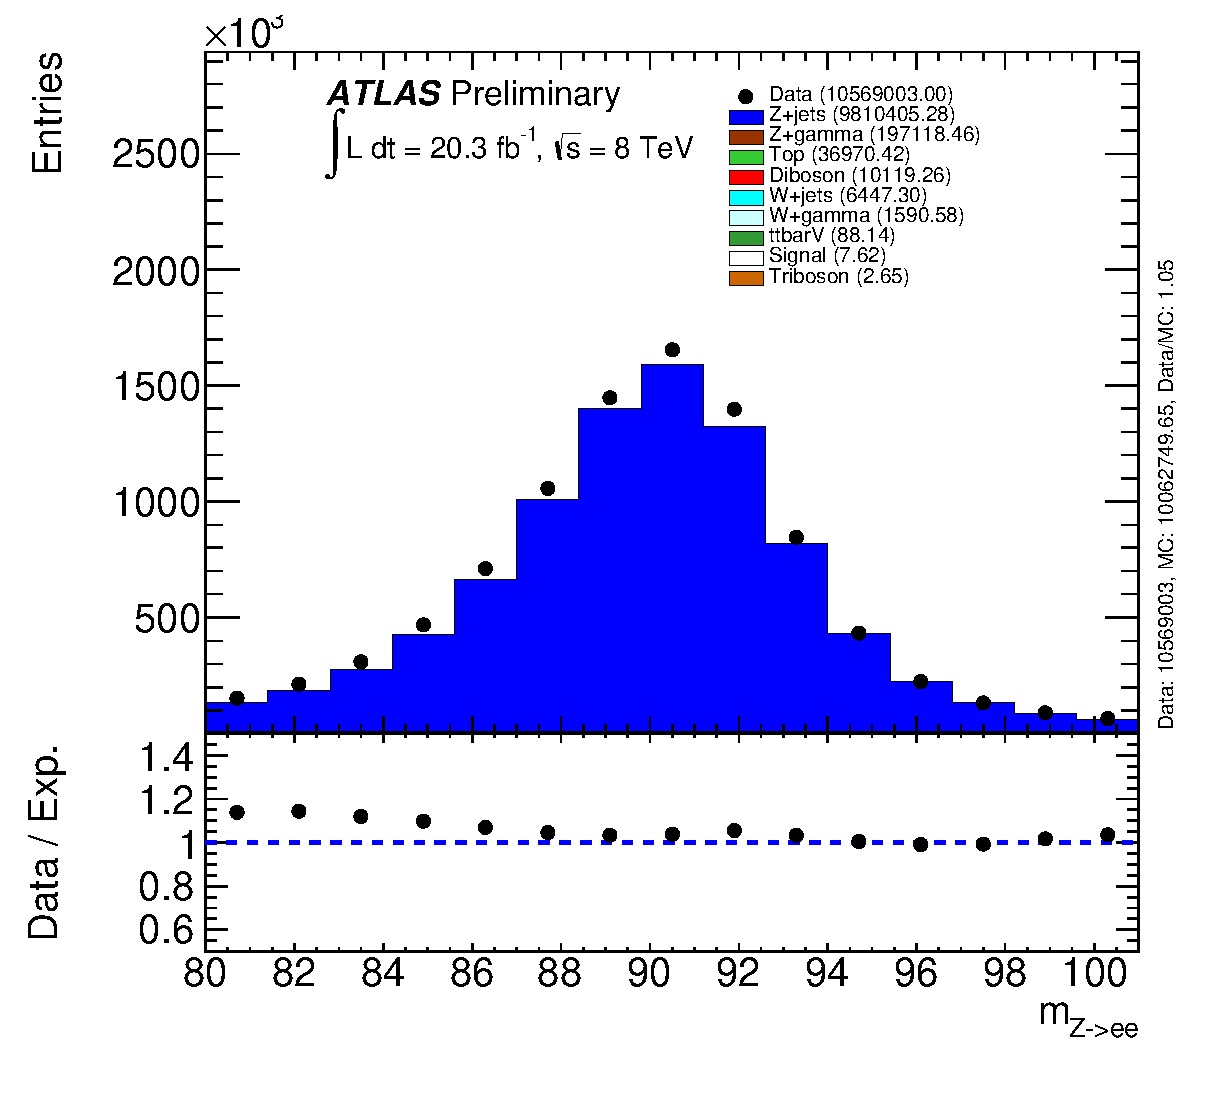
\includegraphics[width=0.4\columnwidth]{figures/fakes_bkg/CRs/hPtElectronZBosonloosecut_total_new.eps}
}
\centering
\subfigure{
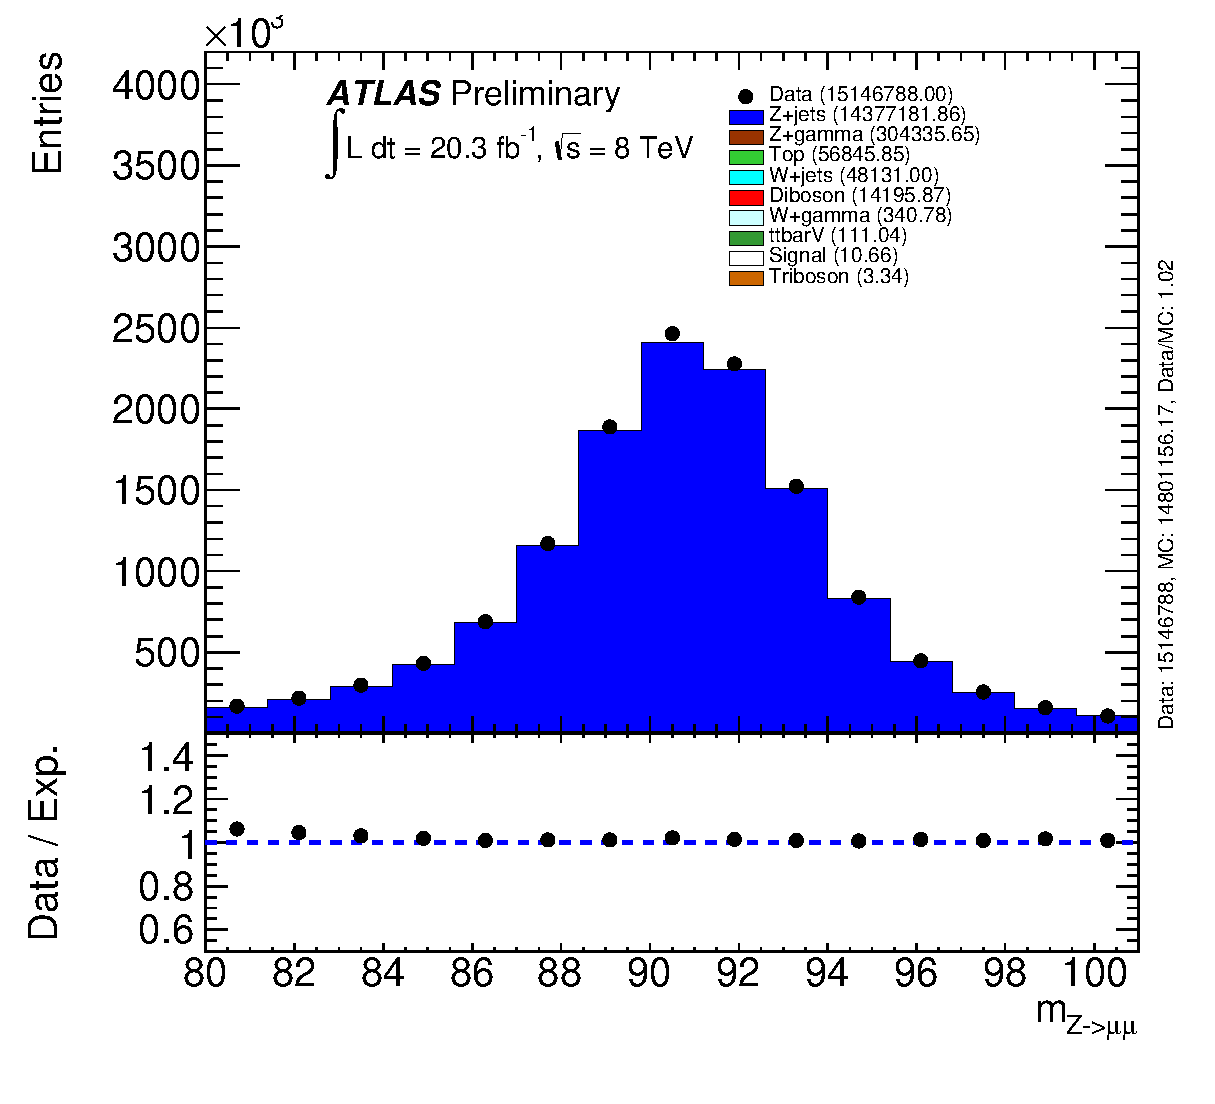
\includegraphics[width=0.4\columnwidth]{figures/fakes_bkg/CRs/hPtMuonZBosonloosecut_total_new.eps}
}
\vspace{-10mm}\caption{Invariant mass distribution of two opposite charge and same flavor di-lepton invariant mass electrons (left) and muons (right).}
\label{fig:realEff_CRs}
\end{figure}


\begin{figure}[h!]
\centering
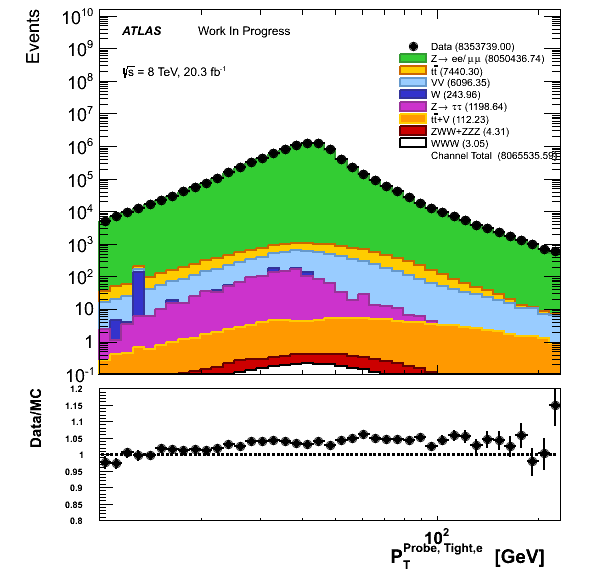
\includegraphics[width=0.4\columnwidth]{figures/fakes_bkg/CRs/RealTP/ProbeTightElectronPt_histratio.png}
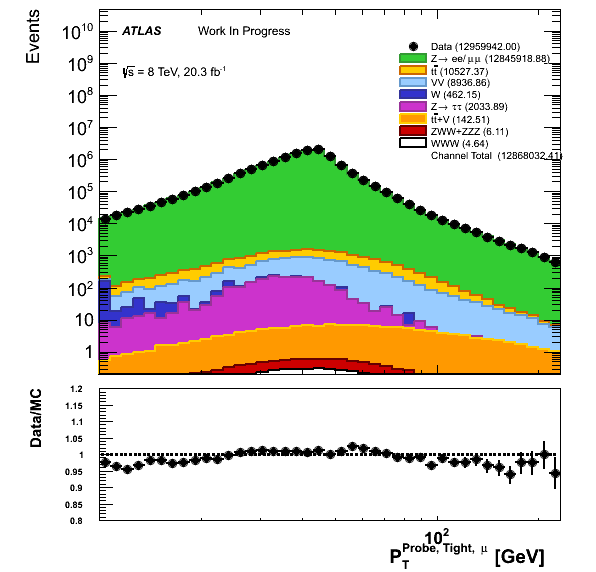
\includegraphics[width=0.4\columnwidth]{figures/fakes_bkg/CRs/RealTP/ProbeTightMuonPt_histratio.png}
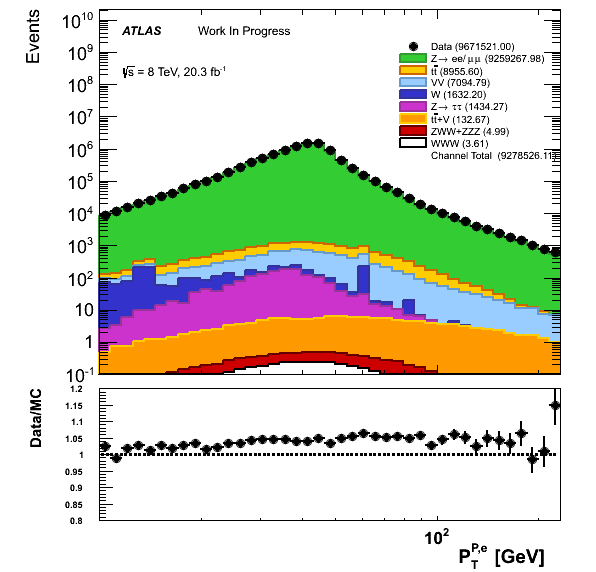
\includegraphics[width=0.4\columnwidth]{figures/fakes_bkg/CRs/RealTP/ProbeElectronPt_histratio.png}
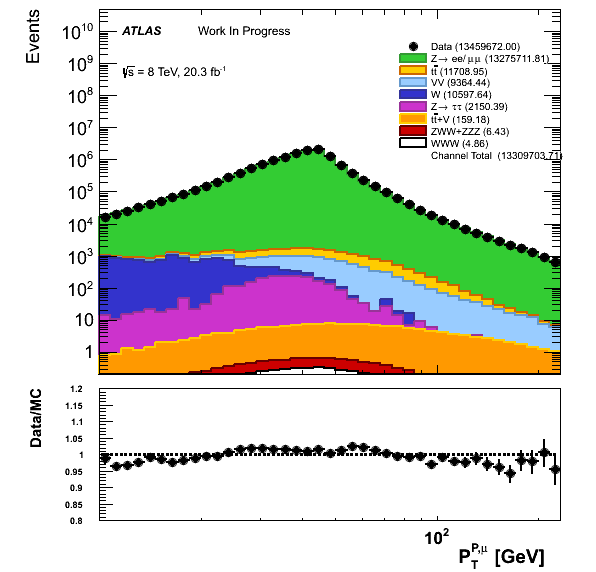
\includegraphics[width=0.4\columnwidth]{figures/fakes_bkg/CRs/RealTP/ProbeMuonPt_histratio.png}
\caption{Probe lepton \pt\ distributions in SFOS tag and probe control regions used to derive real rates.  Electron (left) and muon (right) are shown
when the probe lepton is either tight (top) or no additional selection (besides the preselection) is required (bottom)}
\label{fig:realEff_CRsPt}
\end{figure}


\begin{figure}[h!]
\centering
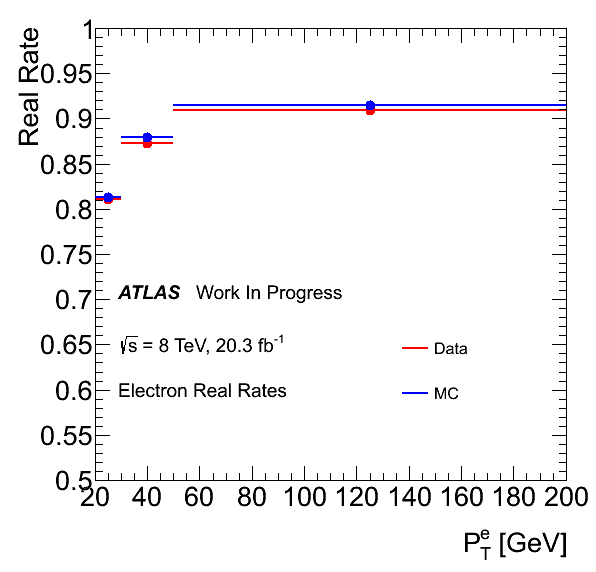
\includegraphics[width=0.45\columnwidth]{figures/fakes_bkg/Efficiencies/ElectronRealRates.png}
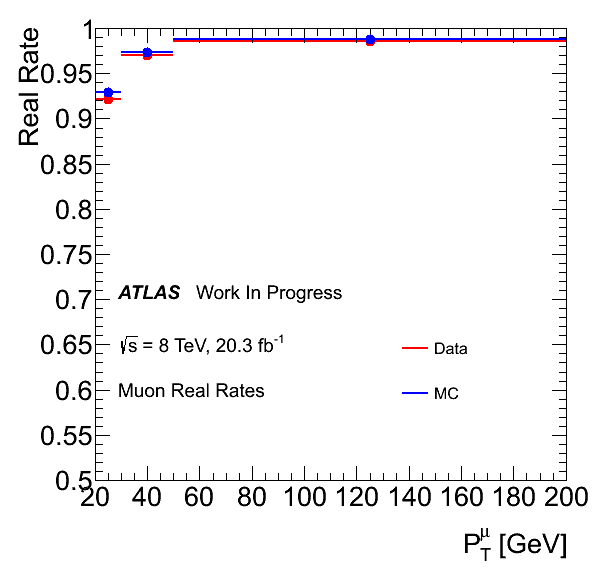
\includegraphics[width=0.45\columnwidth]{figures/fakes_bkg/Efficiencies/MuonRealRates.png}
\caption{Real lepton efficiency as a fucntion of \pt\ and measured in data (red) and MC (blue) for electrons (left) and muons (right).}
\label{fig:realEff}
\end{figure}

\clearpage

%\tabcolsep=0.11cm
\begin{table}[h!]
\centering
\begin{tabular}{|l||c|c||c|c||c|}
\hline
&\multicolumn{2}{c||}{Data}&\multicolumn{2}{c||}{MC}&\multicolumn{1}{c|}{}\\ & $\varepsilon_r$ & $\sigma_{stat}$ & $\varepsilon_r$ & $\sigma_{stat}$ & $\sigma_{sys}$\\ 
\hline\hline
%$p_{T}\in[10,15]$ GeV &  $0.6285$ &  $0.0034$ &  $0.6420$ &  $0.0036$ &  $0.0135$\\ 
%$p_{T}\in[15,20]$ GeV &  $0.6960$ &  $0.0024$ &  $0.7056$ &  $0.0025$ &  $0.0096$\\ 
$p_{T}\in[20,30]$ GeV &  $0.8105$ &  $0.0011$ &  $0.8134$ &  $0.0013$ &  $0.0028$\\ 
$p_{T}\in[30,50]$ GeV &  $0.8732$ &  $0.0005$ &  $0.8794$ &  $0.0006$ &  $0.0062$\\ 
$p_{T} > 50$ GeV &  $0.9097$ &  $0.0012$ &  $0.9150$ &  $0.0012$ &  $0.0053$\\ 
\hline
\end{tabular}

\caption{Measured real efficiencies for electrons including statistical and systematic absolute uncertainties. 
Systematic is calculated by taking the difference
between the efficiencies measured in data and MC.  The efficiency measured in data is used as the nominal central value.
} 
\label{table:realEff_El}
\end{table} 

%\tabcolsep=0.11cm
\begin{table}[h!]
\centering
\begin{tabular}{|l||c|c||c|c||c|}
\hline
&\multicolumn{2}{c||}{Data}&\multicolumn{2}{c||}{MC}&\multicolumn{1}{c|}{}\\ & $\varepsilon$ & $\sigma_{stat}$ & $\varepsilon$ & $\sigma_{stat}$ & $\sigma_{sys}$\\ 
\hline\hline
%$p_{T}\in[10,15]$ GeV &  $0.8684$ &  $0.0033$ &  $0.8763$ &  $0.0036$ &  $0.0079$\\ 
%$p_{T}\in[15,20]$ GeV &  $0.8906$ &  $0.0024$ &  $0.8956$ &  $0.0025$ &  $0.0050$\\ 
$p_{T}\in[20,30]$ GeV &  $0.9217$ &  $0.0010$ &  $0.9291$ &  $0.0012$ &  $0.0074$\\ 
$p_{T}\in[30,50]$ GeV &  $0.9700$ &  $0.0004$ &  $0.9737$ &  $0.0006$ &  $0.0038$\\ 
$p_{T} > 50$ GeV &  $0.9862$ &  $0.0011$ &  $0.9878$ &  $0.0011$ &  $0.0017$\\ 
\hline
\end{tabular}

\caption{Measured real efficiencies for muons including statistical and systematic absolute uncertainties.
Systematic is calculated by taking the difference
between the efficiencies measured in data and MC.  The efficiency measured in data is used as the nominal central value.
} 
\label{table:realEff_Mu}
\end{table} 


\clearpage

\subsubsection{Fake lepton efficiency}

The fake efficiency represents the probability that a fake lepton satisfying the preselected criteria passes also the signal requirements. 
The measurement, performed separately for each $\pt$ bin, $i$, is performed in fake-enriched samples by looking at the number of probe leptons in data 
passing preselection, $n_i$, and comparing to the number which only pass also the tight
selection, $n^{Tight}_i$. Contamination from real leptons, $n^{\mathrm{Real}}_i$ and $n^{\mathrm{Tight}, \mathrm{Real}}_i$, 
and from photon converted leptons, $n^{\mathrm{PC}}_i$ and $n^{\mathrm{Tight},\mathrm{PC}}_i$, 
is corrected using MC by subtracting from the totals.  The rate is then determined as follows:
%\begin{align*}
\begin{equation}
\zeta_i=\frac{n^{\mathrm{Tight}}_i-n^{\mathrm{Tight},\mathrm{Real}}_i-n^{\mathrm{Tight},\mathrm{PC}}_i} {n_i -n^{\mathrm{Real}}_i -n^{\mathrm{PC}}_i }
\label{eq:fakerate}
\end{equation}
%\end{align*}
Since the rates depend on the fake lepton origin, the derivation is done separately for electrons and muons.     

The classification of leptons in MC as being either real or from photon conversion is performed on an event-by-event basis at truth level using the MCTruthClassifier tool~\cite{MCtruthclassifier:twiki}.  
Since this is a dilepton control region, the majority of events with a real lepton
tag and a probe lepton due to photon conversion comes from the $W\gamma$ process where the photon converted lepton is an electron.
As expected, the number of probe muons coming from photon conversion are observed to be negligible.

Efficiencies are measured from a data set enriched with one tight lepton that passes the signal lepton selections with \pt$>40$~\GeV\ and 
one fake candidate satisfying only the preselection criteria defined in tables~\ref{tab:eledef} and~\ref{tab:muondef}. Events with additional loose or tight leptons are rejected. 
The QCD background may also enter these control regions, especially in low \met\ . Therefore, an additional \met$>10$~\GeV\ requirement is introduced. 
In order to reduce the contamination from real processes like $t\bar{t}$, $WW$ and $Z$, the two leptons are required to have the same sign.
Finally, the control regions are split based on the flavor of the tag and probe leptons.  The muon rates are determined in the region
with two muons while the electron rates are determined in the region with a muon tag and an electron probe.  The choice of a muon tag 
in the region used to derive the electron rates is particularly important since allowing electron tags have a large contamination from $Z$ backgrounds.
This is true even after the same-sign requirement because of charge mis-identification.  
The charge mis-identification rate for muons is negligible
and so allows one to use the muon-muon control region for the muon rates, which has the least contamination.
This behavior can be seen in the distributions of probe muon transverse momentum in the same-sign muon-muon tag-and-probe control region used to derive
the muon fake rates shown in Fig.~\ref{fig:fakeEff_CRs_muon} while
the distributions of probe electron transverse momentum are shown in the same-sign electron-muon tag-and-probe control region used to derive
the electron fake rates shown in Fig.~\ref{fig:fakeEff_CRs_electron}.
The control regions for both electrons and muons are further split based on the number of b-tagged jets in the event, 
which has an effect on the source of the fake leptons.  In particular, requiring b-tagged jets increases the fraction
of fake leptons coming from heavy flavor. Two different sets of control regions were ultimately considered, those
with at least one b-tagged jet and those without any requirement on the presence of b-tagged jets.  The region
with at least one b-tagged jet ($N_{b-jet} > 0$) is used as the central value since it contains more heavy flavor contributions
and so compares better with the signal regions, as described later in Section~\ref{sec:fakecomposition}.  The other is used 
to determine a systematic on the composition, described later.  


A detailed breakdown of the numbers used to compute the fake rates are shown in Appendix~\ref{sec:appendix_fakebg}.
%would it be useful to show the other dilepton control regions in an appendix?

Three systematic uncertainties are considered. First, the subtraction of the processes with 
two real leptons ($t\bar{t}V$, $VV$ and $VVV$) using MC prediction introduced an uncertainty on 
their cross-sections. This effect is estimated by varying the MC normalization by $\pm 20$\%.  %should rerun with 5%
We refer to this is as the 'correlated' systematic uncertainty.
Second, given that the extraction regions and the signal regions have different kinematic selections, 
the fake leptons of different origin dominate. This kinematic dependence of fake efficiencies has been estimated 
by modifying the requirements of the sample used for the measurement. In particular, the cut thresholds 
on the $E_{T}^{Miss}$ and tag lepton $\pt$ used
for determining the dilepton control regions are varied. The $E_{T}^{Miss}$ threshold is 
varied in 5~GeV steps scanning a range of $\pm 10$~GeV around the nominal
threshold of $E_{T}^{Miss} > 10$~GeV while the $\pt$ threshold is varied in 5~GeV steps in a range of $\pm 20$~GeV 
around the nominal threshold of $\pt > 40$~GeV.  When varying the $E_{T}^{Miss}$ cut, the $\pt$ cut
is kept at the nominal threshold and vise-versa. This is referred to as the 'uncorrelated' systematic.
These are determined separtely for electrons and muons, since they use different control regions. The 'uncorrelated' and
'correlated' systematics for electrons and muons are then combined together by adding in quadrature on an event-by-event basis.
As a result the uncertainty is presented as a single systematic uncertainty on the fake electron
contribution and a separte single systematic on the fake muon contribution.
The third and final systematic contribution comes from the choice of control region, based on the number of b-tagged
jets, as described earlier.  The nominal control regions for both the electron and muon cases is when 
there is at least one b-tagged jet present.  The difference between the rates for the nominal case
and the region where no requirement is placed on the presence of b-tagged jets is chosen as a systematic.
We have determined that the difference in the composition in these two regions adequately covers the difference
in composition that may be present due to the extrapolation from the control regions to the signal regions. This is 
discussed in more detail in Section~\ref{sec:fakecomposition}.  Another set of control regions was studied
which vetos any b-tagged jets, but this was observed to give a very large difference in composition which is 
probably too conservative of an estimate to be used as a reasonable systematic.
The rates along with the statistical and systematic uncertainties are summarized in Fig.~\ref{fig:fakeEff} 
as well as in Tables \ref{table:fakeEff_El} and \ref{table:fakeEff_Mu}.
The final binning of the efficiency is chosen to be coarse enough
to have good statistics in the ratio while also preserving shape information as a function
of $\pt$. 


%\begin{figure}[h!]
%\centering
%\subfigure{
%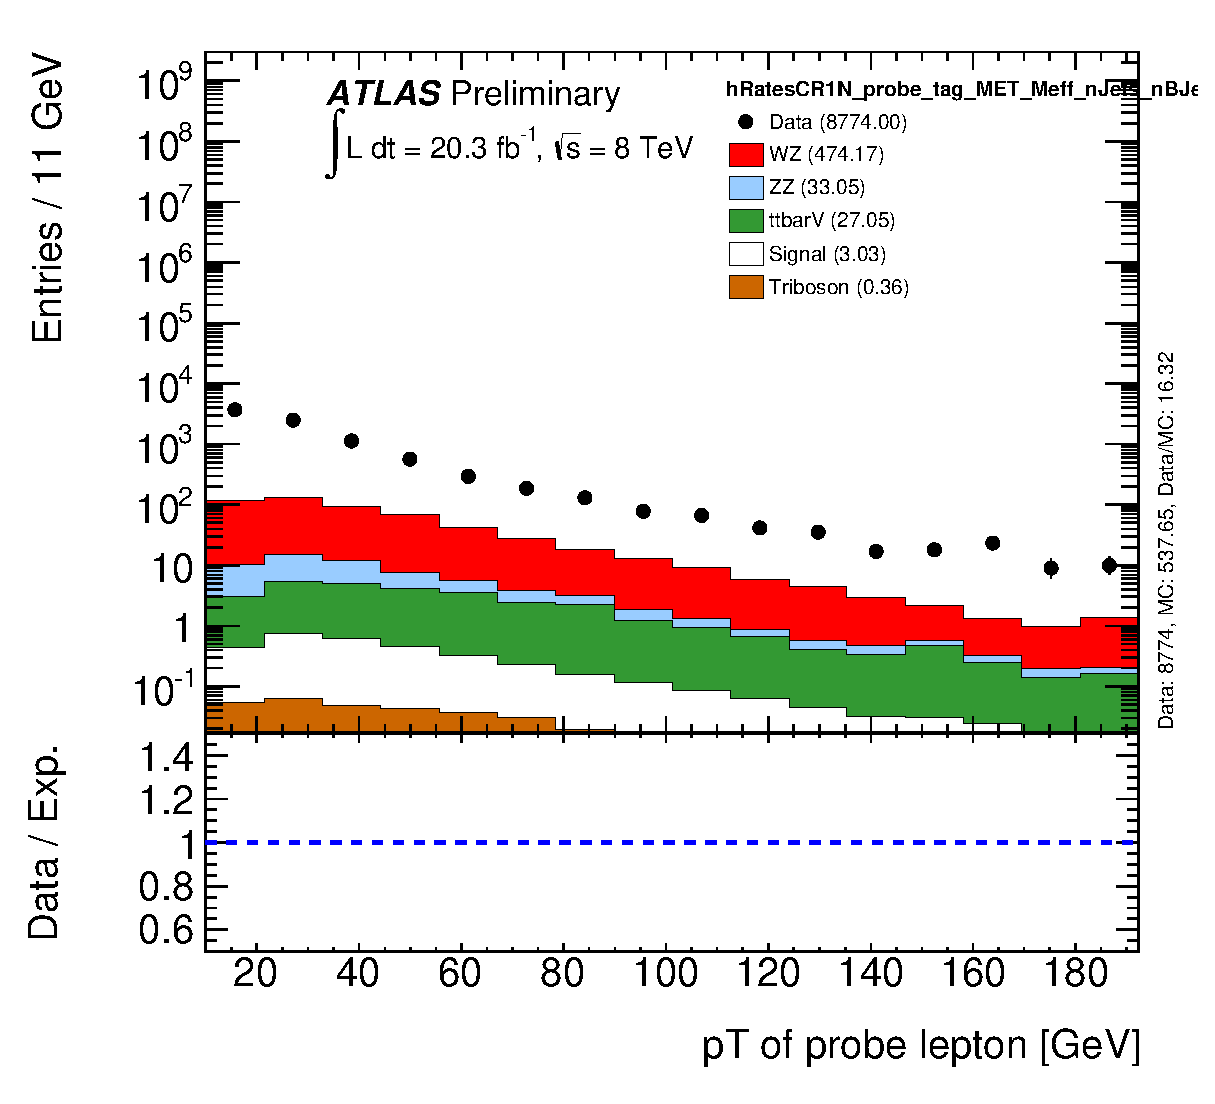
\includegraphics[width=0.3\columnwidth]{figures/fakes_bkg/CRs/CR1N_probePt_all_total.eps}
%}
%\centering
%\subfigure{
%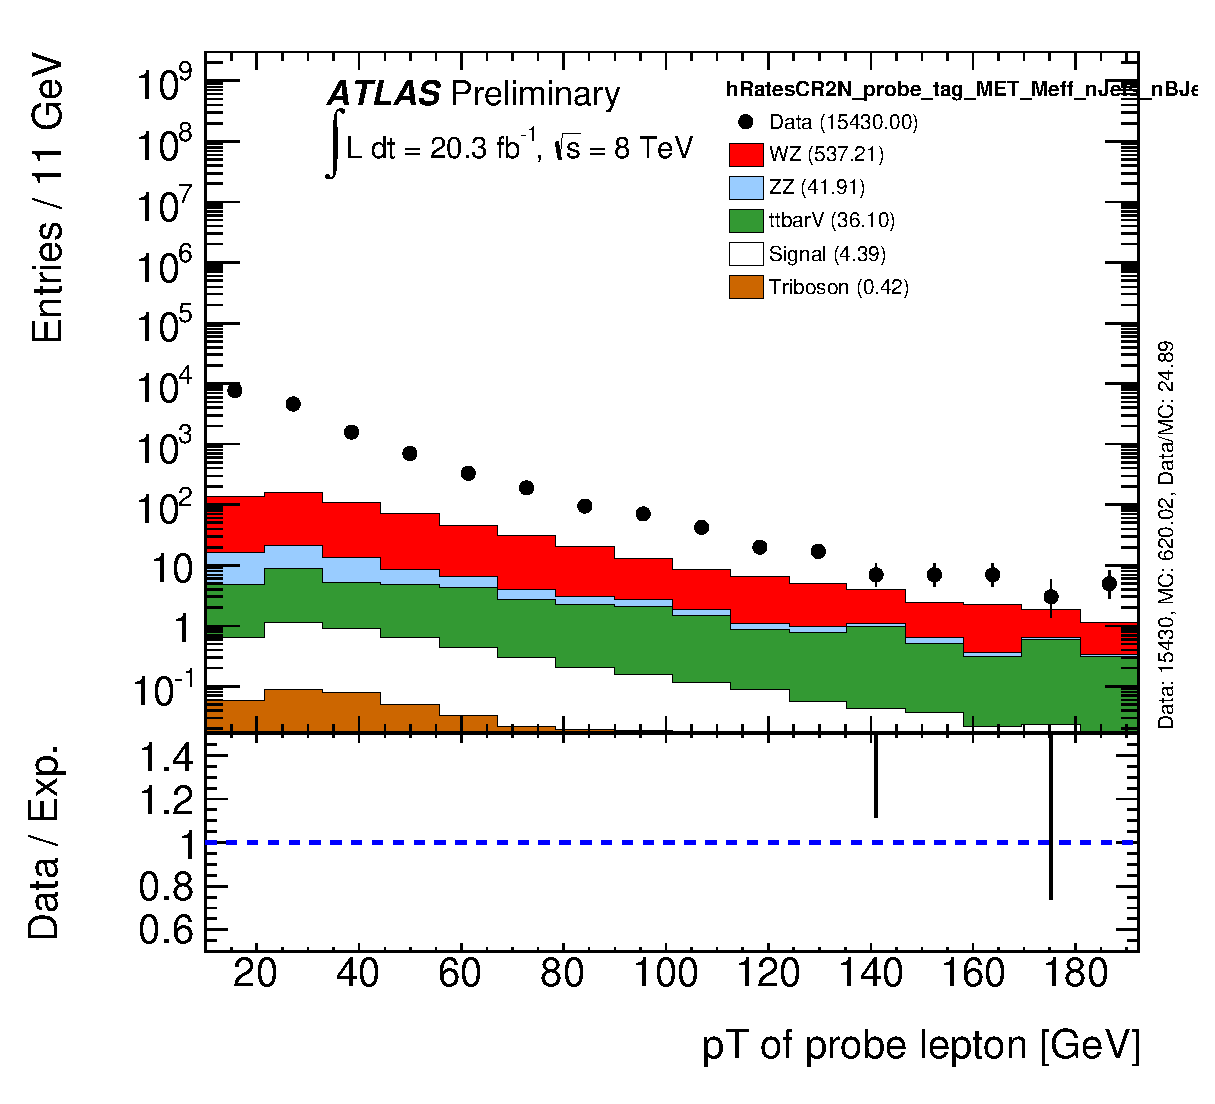
\includegraphics[width=0.3\columnwidth]{figures/fakes_bkg/CRs/CR2N_probePt_all_total.eps}
%}\\ 
%\vspace{-14mm}
%\subfigure{
%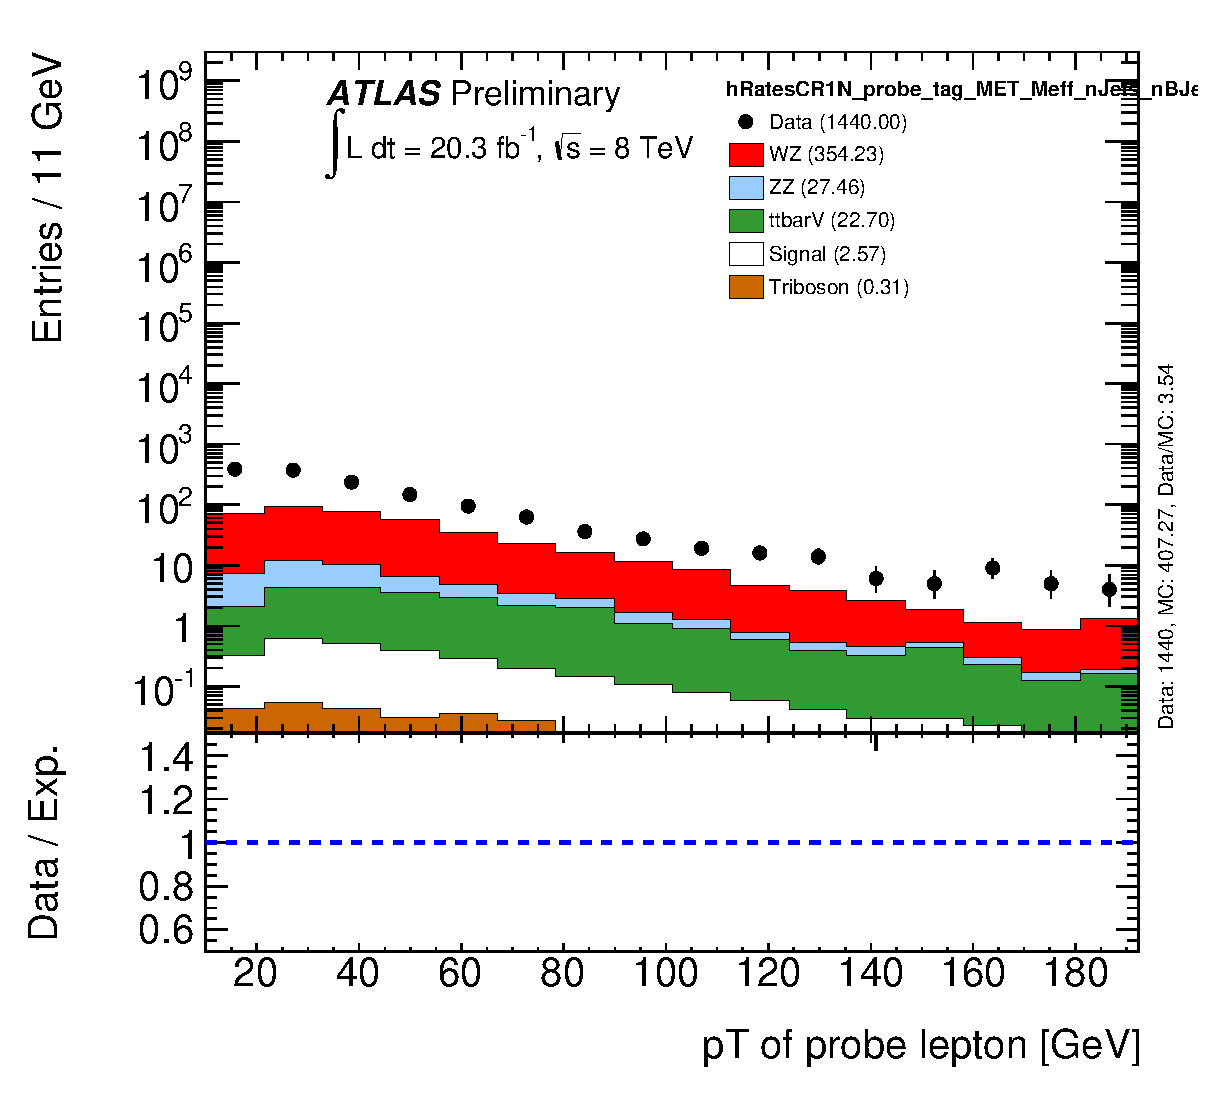
\includegraphics[width=0.3\columnwidth]{figures/fakes_bkg/CRs/CR1N_probePt_tight_total.eps}
%}
%\centering
%\subfigure{
%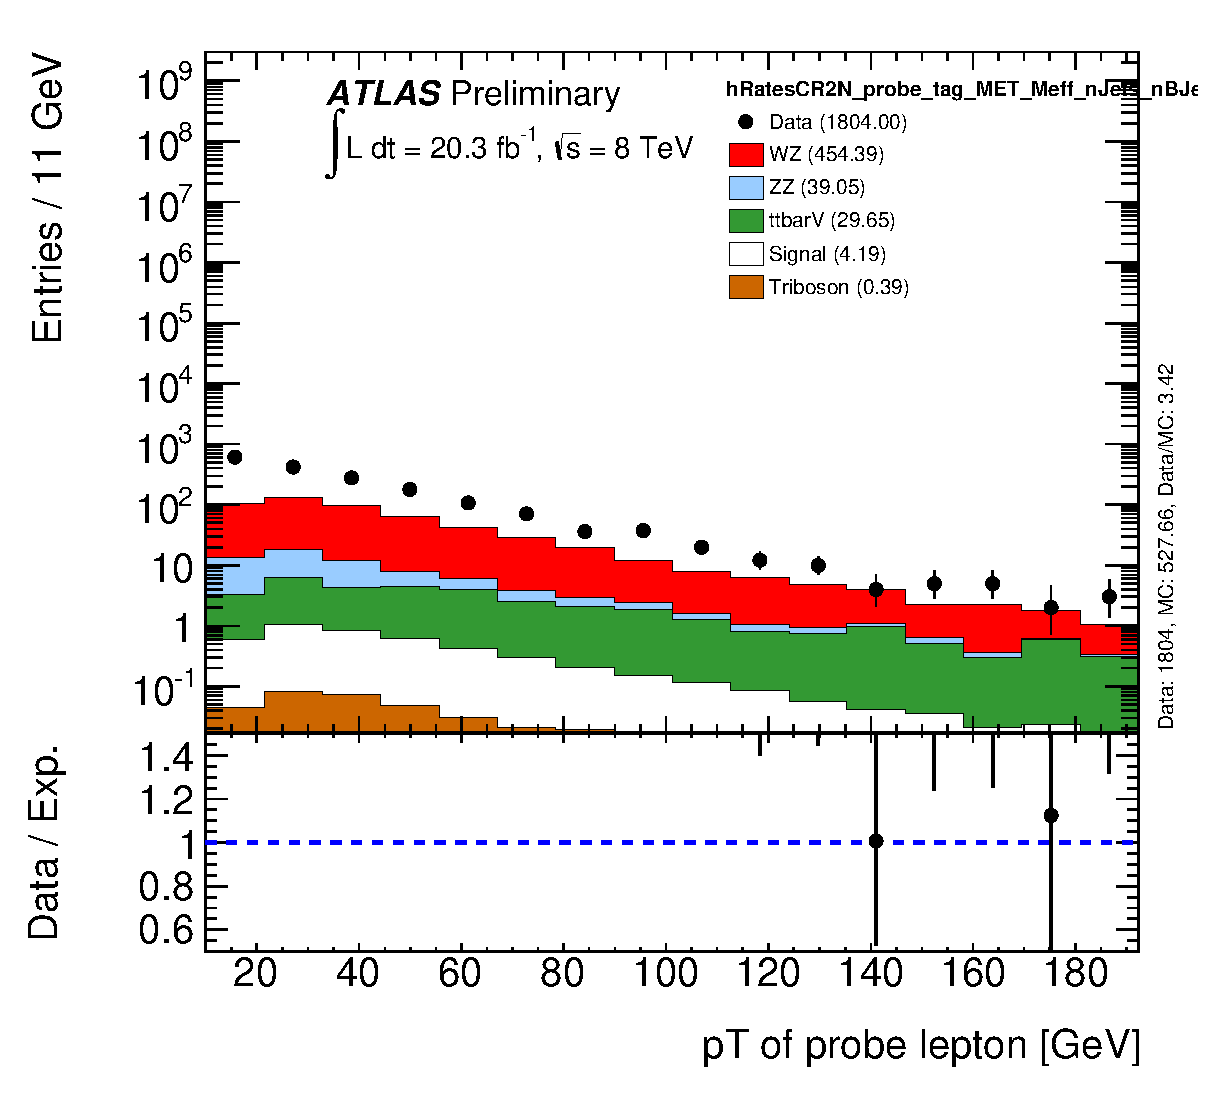
\includegraphics[width=0.3\columnwidth]{figures/fakes_bkg/CRs/CR2N_probePt_tight_total.eps}
%}
%\vspace{-10mm}\caption{Transverse momentum distributions \pt\ of probe electron (left) and muon (right) in the control regions. The probe passes pre-selection (top) and signal (bottom) criteria.}
%\label{fig:fakeEff_CRs}
%\end{figure}


\begin{figure}[h!]
\centering
\subfigure{
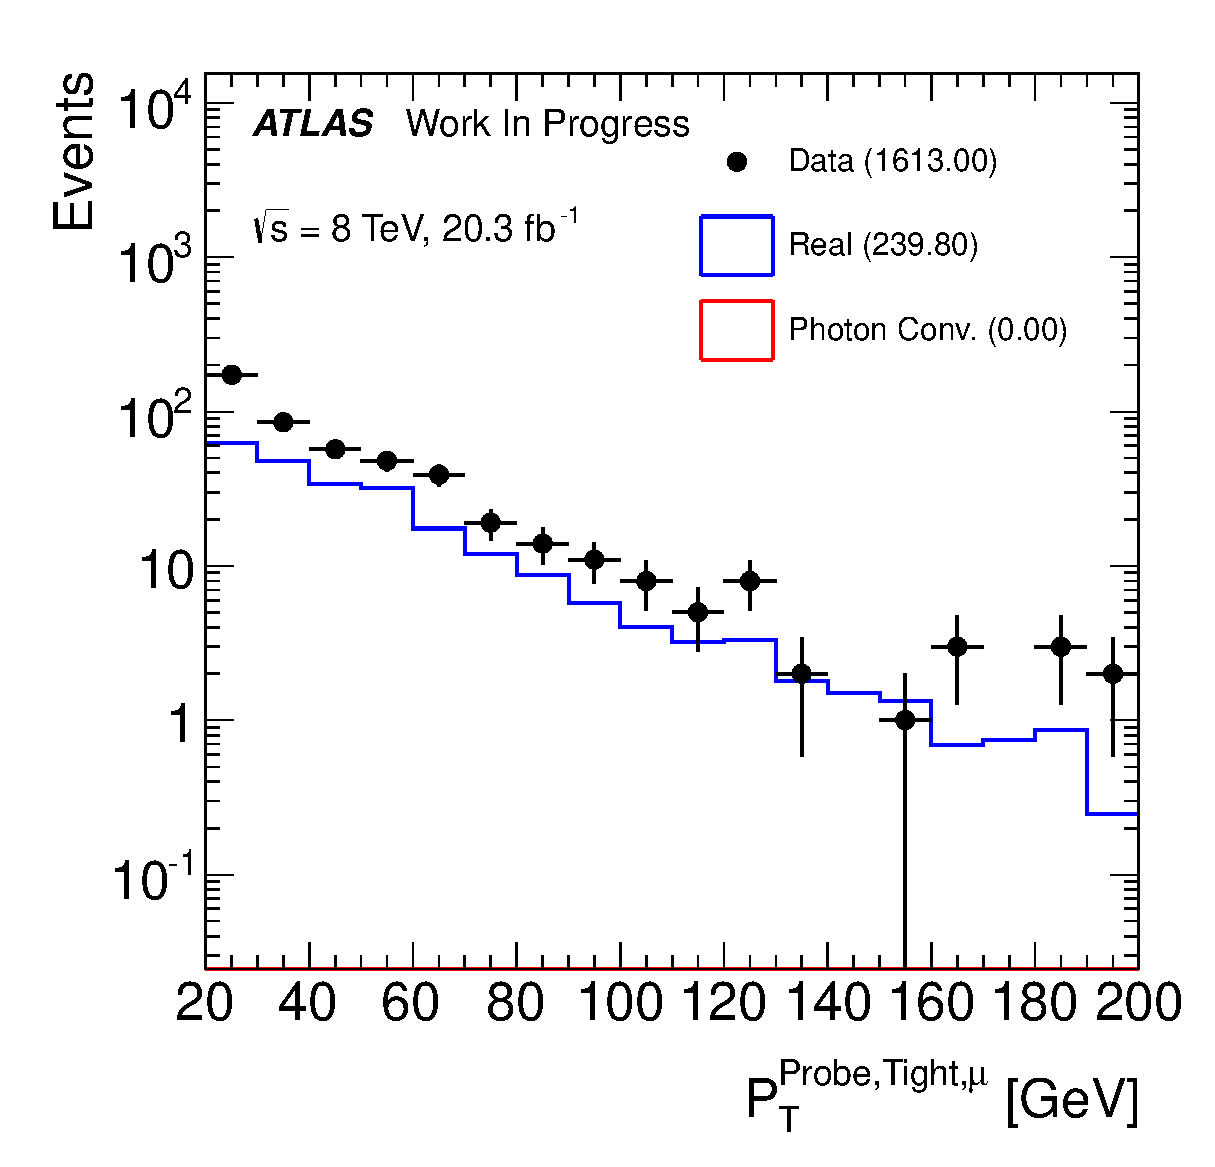
\includegraphics[width=0.45\columnwidth]{figures/fakes_bkg/CRs/SameSignMuonMuon/NoStack/ProbeTightMuonPt.eps}
}
%\centering
%\subfigure{
%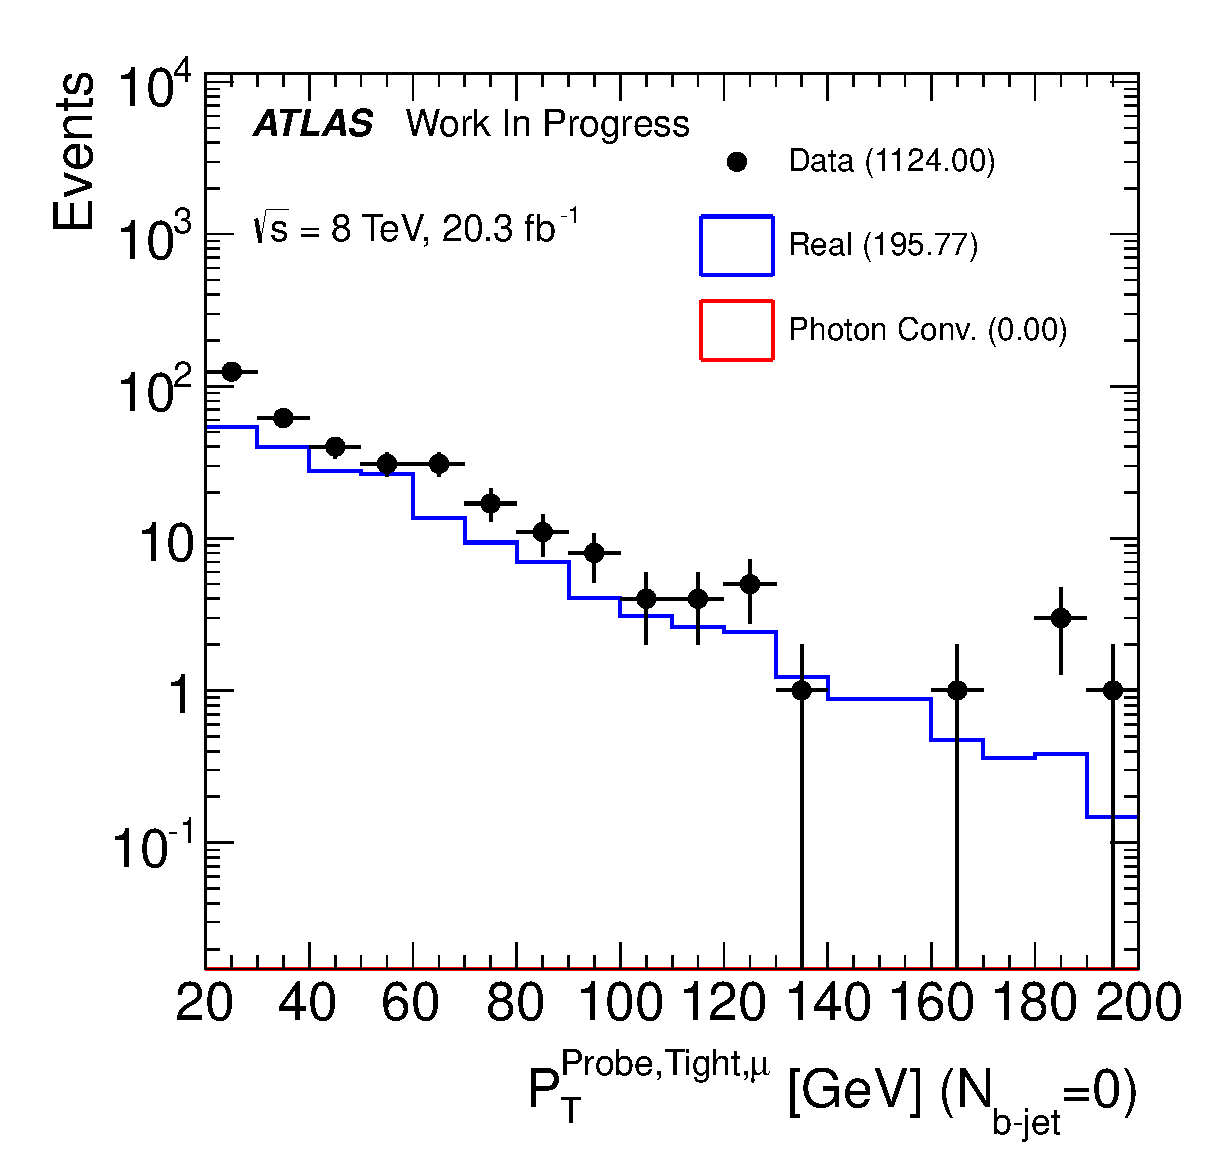
\includegraphics[width=0.3\columnwidth]{figures/fakes_bkg/CRs/SameSignMuonMuon/NoStack/ProbeTightMuonPtBJetEq0.eps}
%}
\centering
\subfigure{
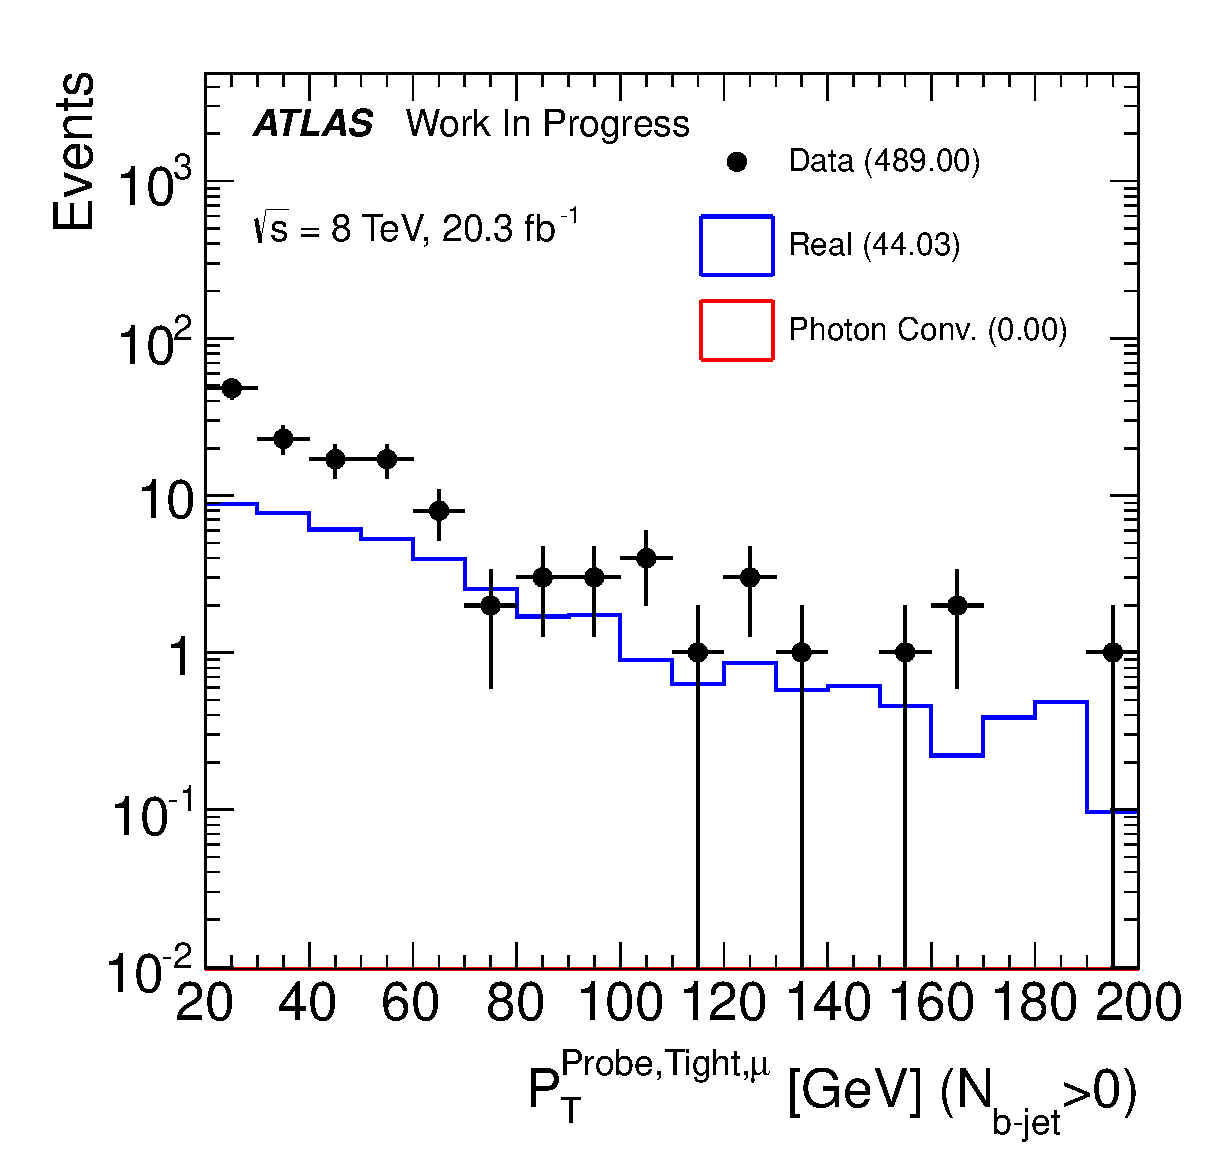
\includegraphics[width=0.45\columnwidth]{figures/fakes_bkg/CRs/SameSignMuonMuon/NoStack/ProbeTightMuonPtBJetGt0.eps}
}
%\vspace{-1mm}
\centering
\subfigure{
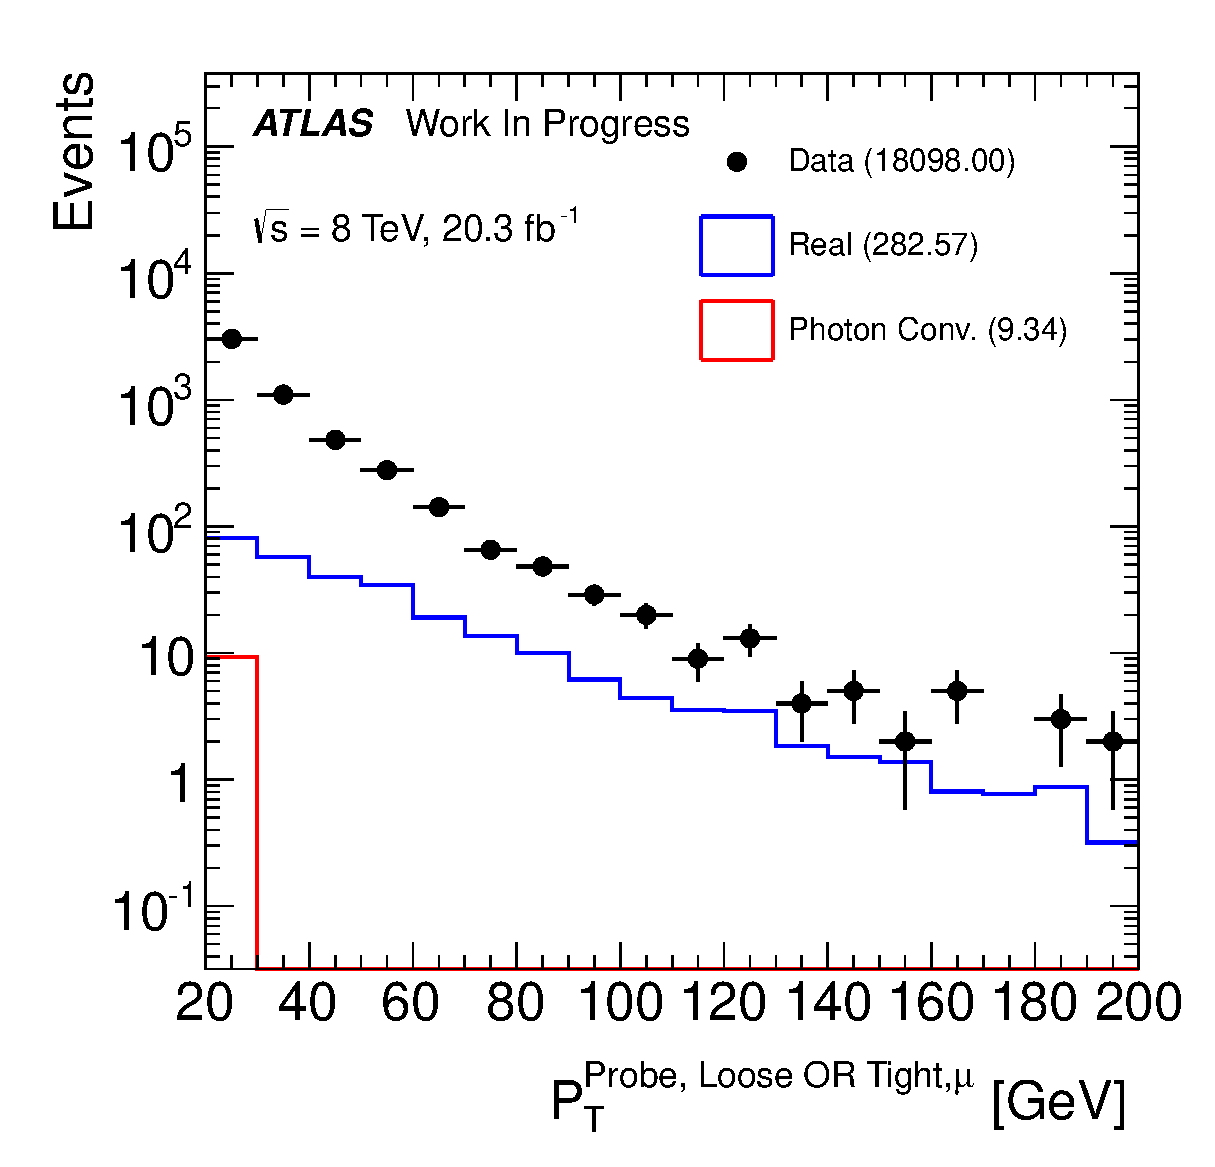
\includegraphics[width=0.45\columnwidth]{figures/fakes_bkg/CRs/SameSignMuonMuon/NoStack/ProbeLooseORTightMuonPt.eps}
}
%\centering
%\subfigure{
%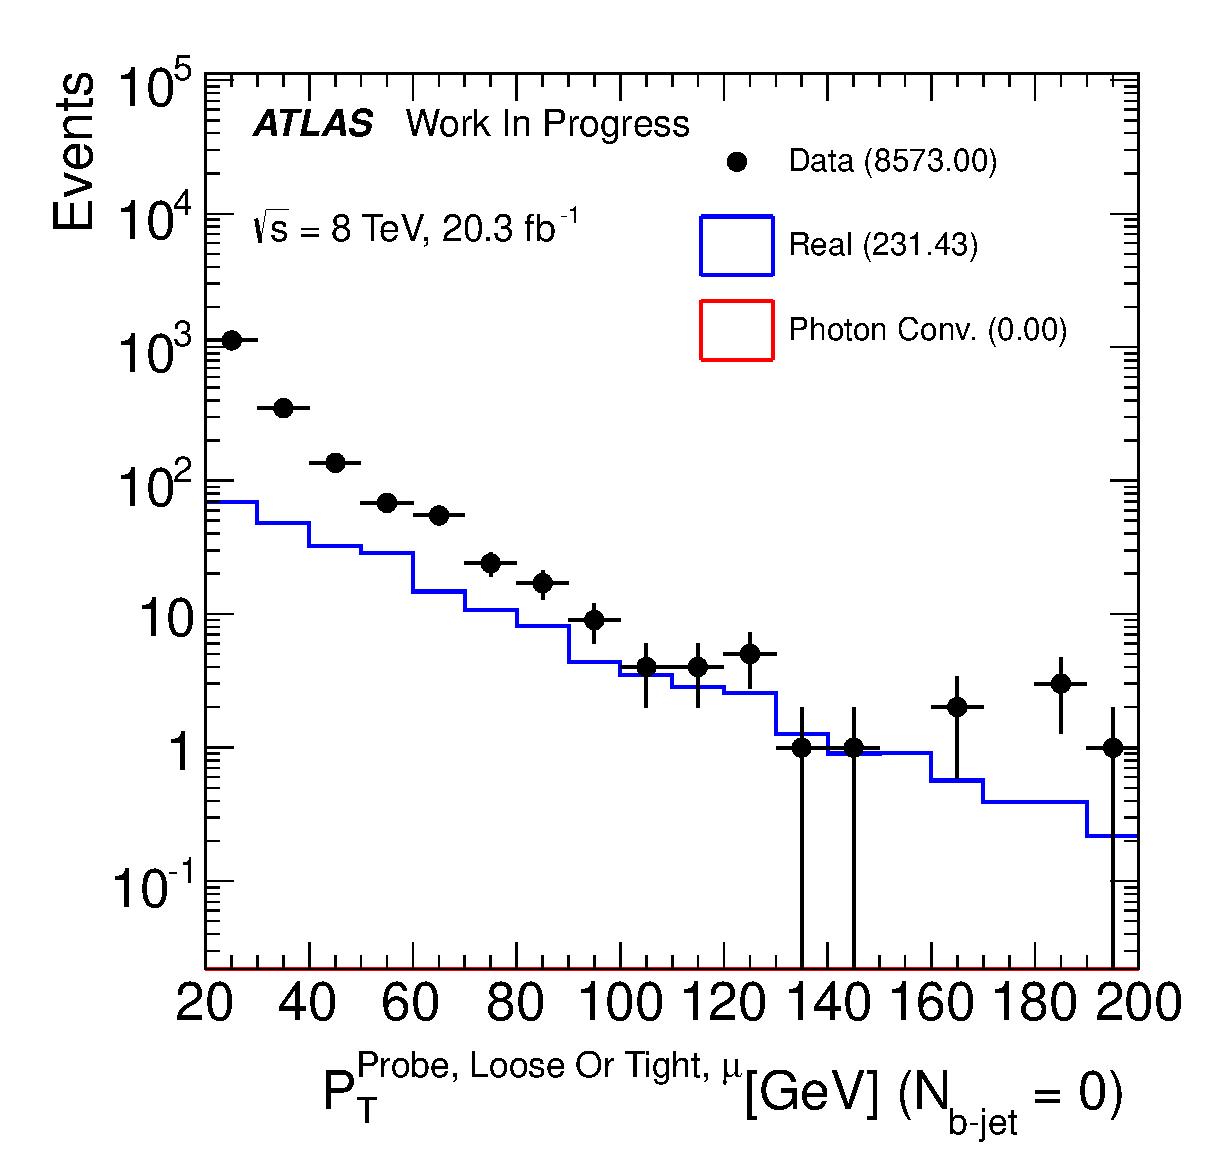
\includegraphics[width=0.45\columnwidth]{figures/fakes_bkg/CRs/SameSignMuonMuon/NoStack/ProbeLooseORTightMuonPtBJetEq0.eps}
%}
\centering
\subfigure{
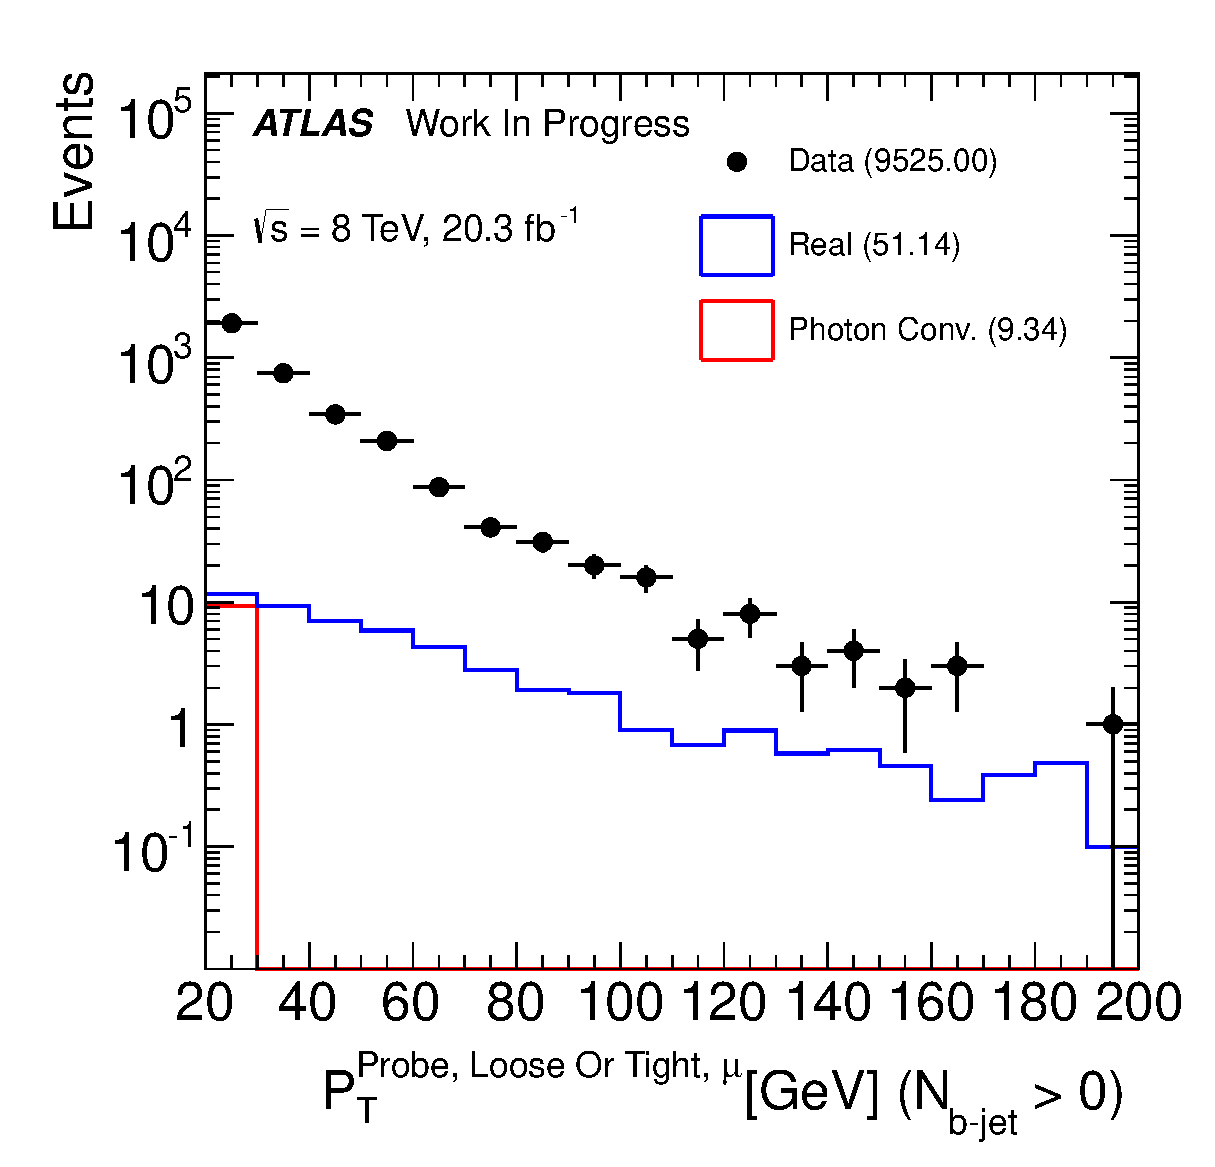
\includegraphics[width=0.45\columnwidth]{figures/fakes_bkg/CRs/SameSignMuonMuon/NoStack/ProbeLooseORTightMuonPtBJetGt0.eps}
}
\vspace{-10mm}\caption{Transverse momentum distributions \pt\ of tight probe muons (top) and loose OR tight probe muons (bottom) passing signal selection criteria in the control Same-Sign $\mu-\mu$ control region without any additional requirement on $b$-jets in the event (left) and at least one $b$-jet (right). 
The amount observed in data (black points) corresponds to $n$ (bottom) and $n_{\textrm{Tight}}$ (top) in Eq.~\ref{eq:fakerate}. 
Meanwhile, the contribution determined in MC to come from real leptons (blue line) and from photon conversion (red line) are shown 
separately; they are not stacked. The real lepton contribution corresponds to 
$n_{\textrm{Tight}}^{\textrm{Real}}$ (top) and $n^{\textrm{Real}}$ (bottom) and the photon conversion 
contribution corresponds to $n_{\textrm{Tight}}^{\textrm{PC}}$ (top) and $n^{\textrm{PC}}$ (bottom) in Eq.~\ref{eq:fakerate}. The photon conversion is 
observed to be negligible for muons.  }
\label{fig:fakeEff_CRs_muon}
\end{figure}

\begin{figure}[h!]
\centering
\subfigure{
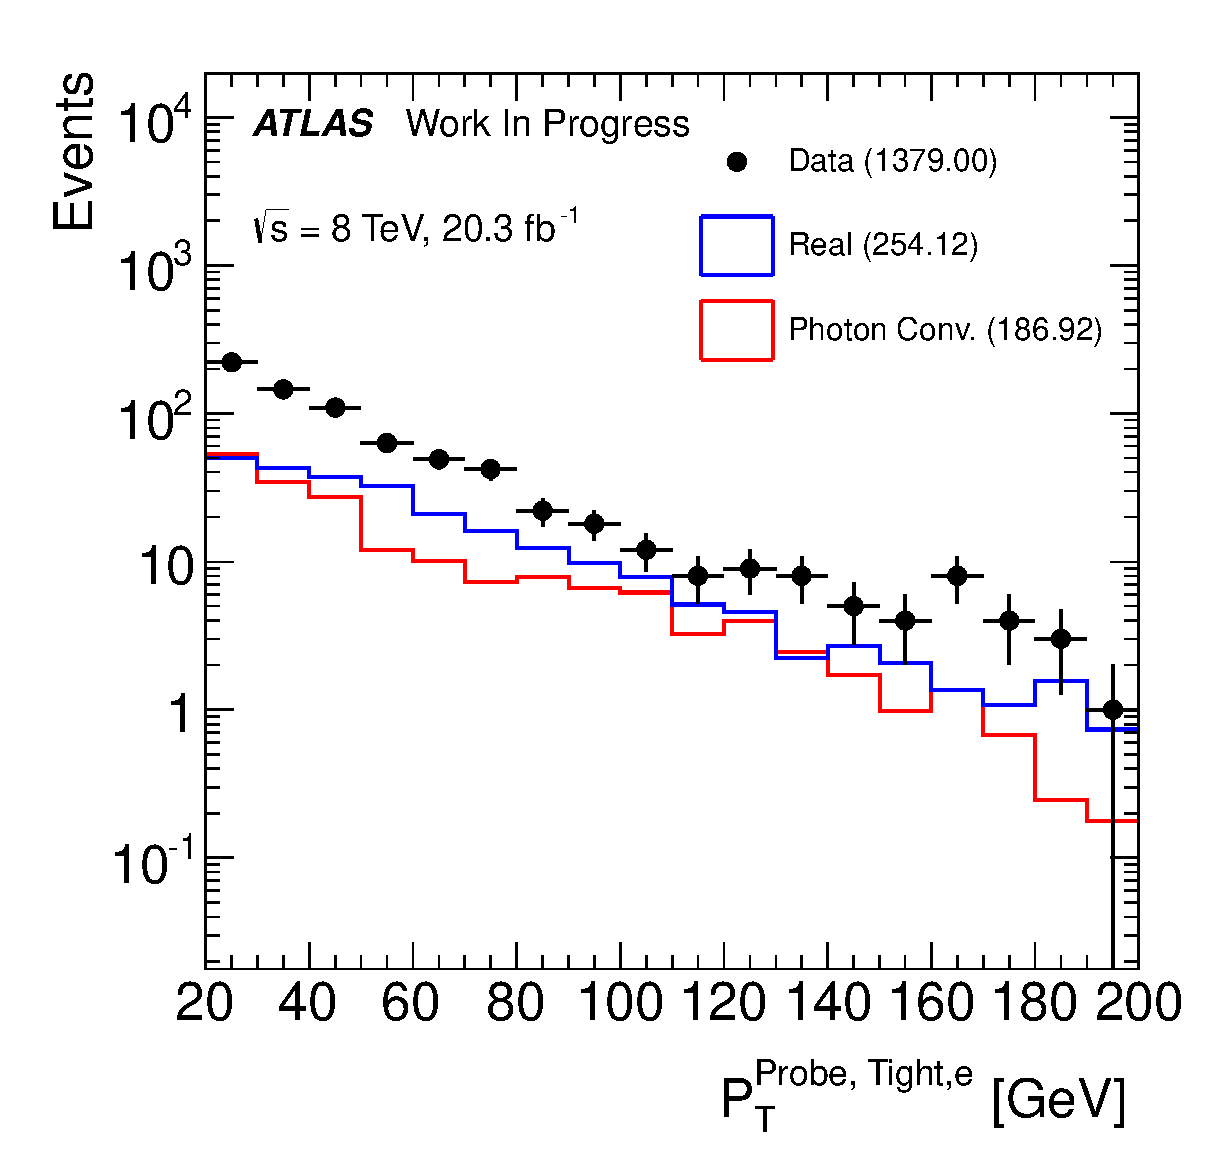
\includegraphics[width=0.45\columnwidth]{figures/fakes_bkg/CRs/SameSignElectronMuon/NoStack/ProbeTightElectronPt.eps}
}
%\centering
%\subfigure{
%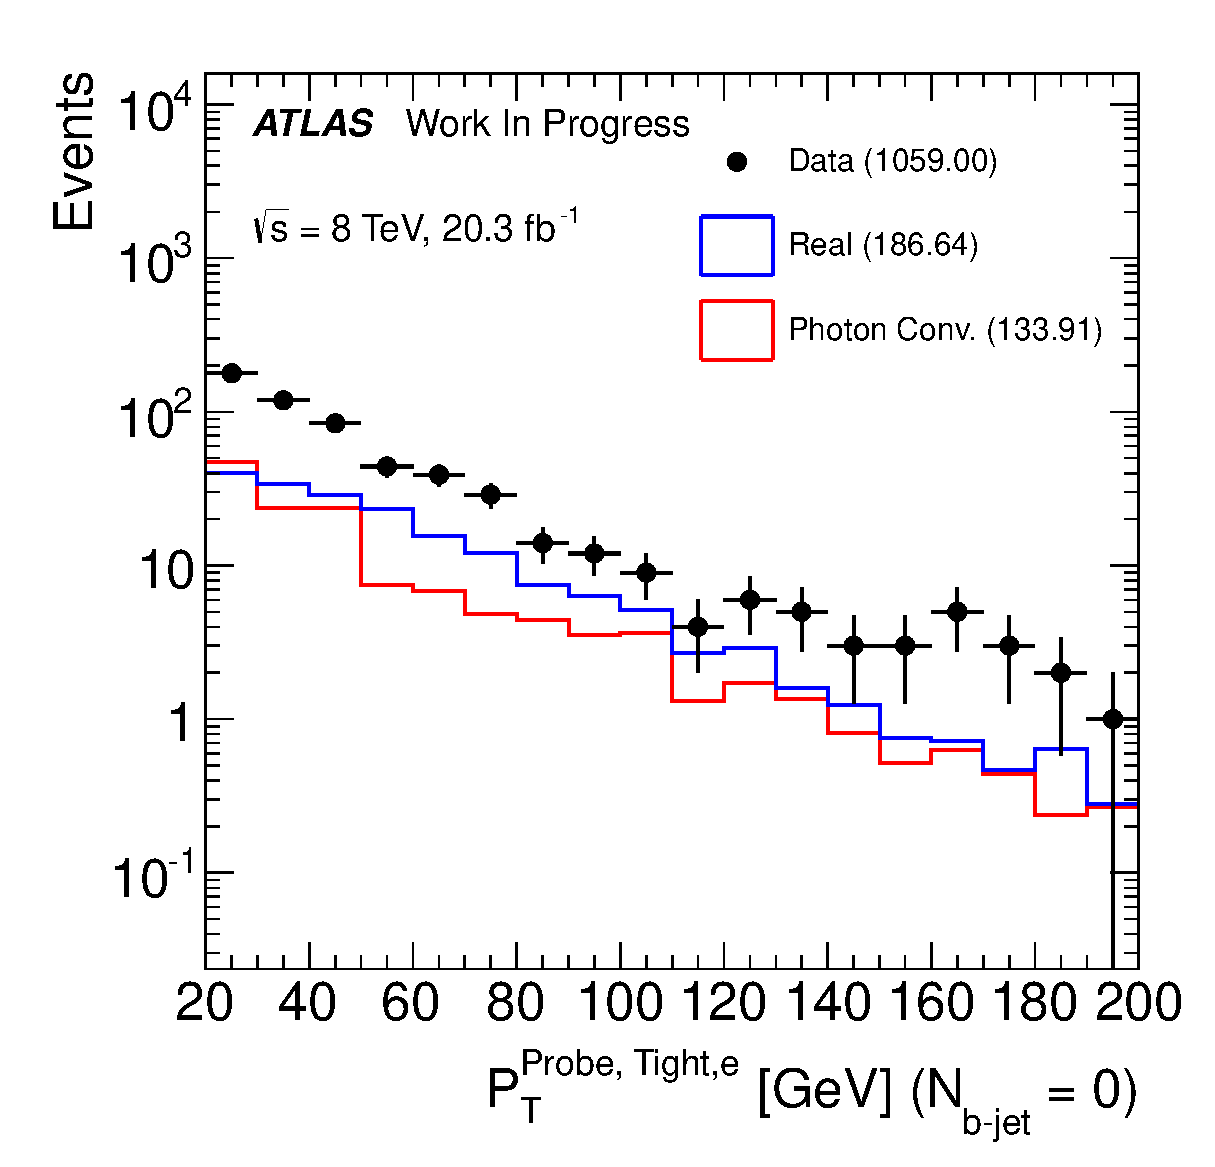
\includegraphics[width=0.3\columnwidth]{figures/fakes_bkg/CRs/SameSignElectronMuon/NoStack/ProbeTightElectronPtBJetEq0.eps}
%}
\centering
\subfigure{
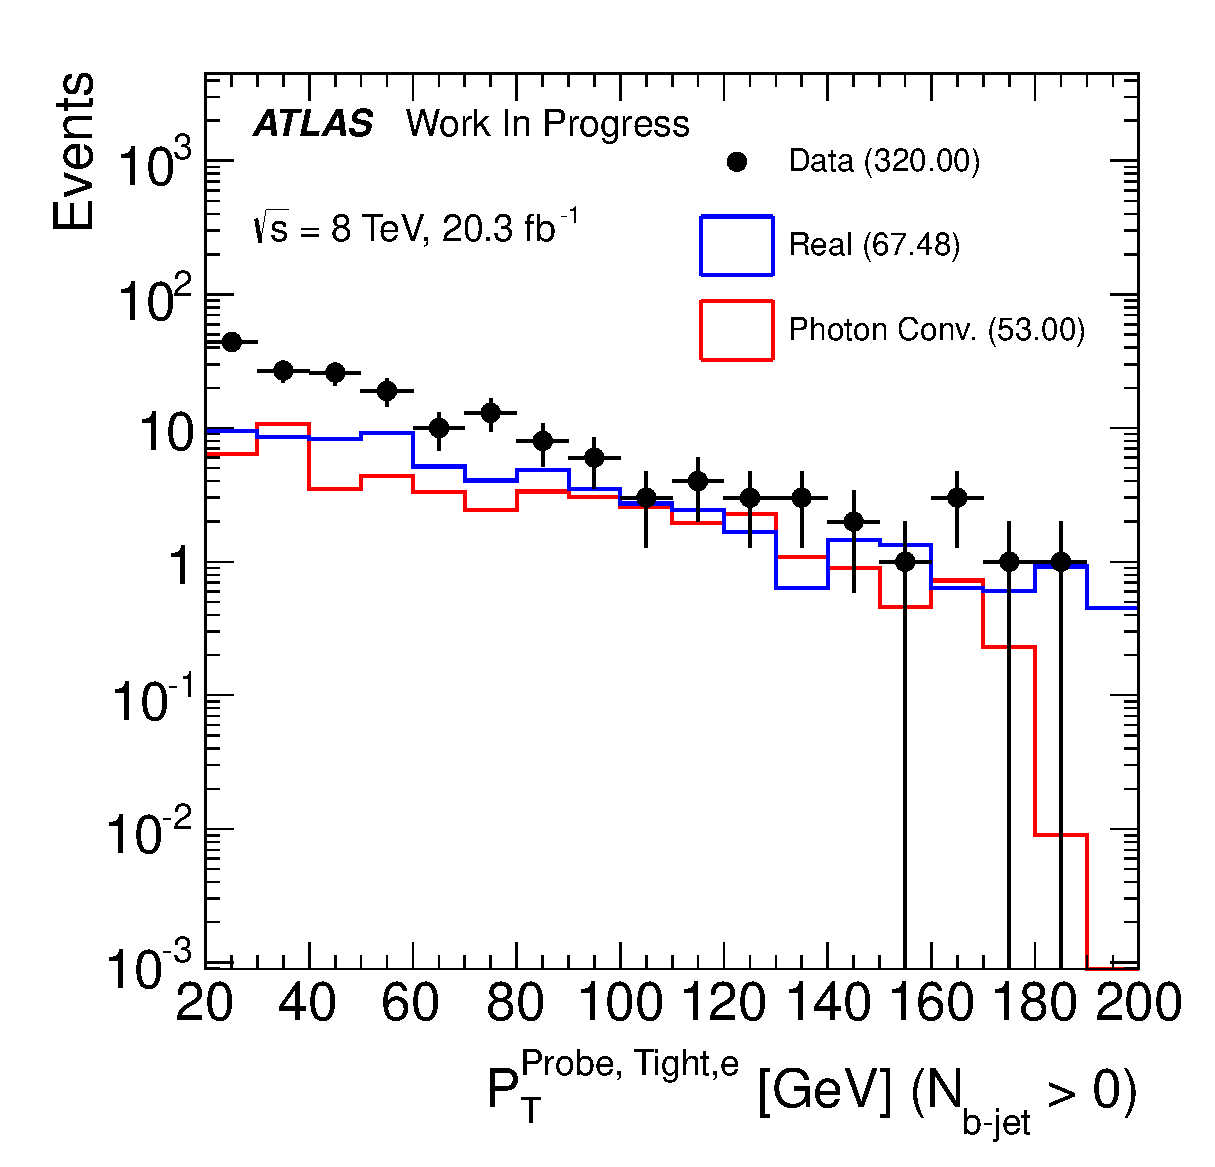
\includegraphics[width=0.45\columnwidth]{figures/fakes_bkg/CRs/SameSignElectronMuon/NoStack/ProbeTightElectronPtBJetGt0.eps}
}
\centering
\subfigure{
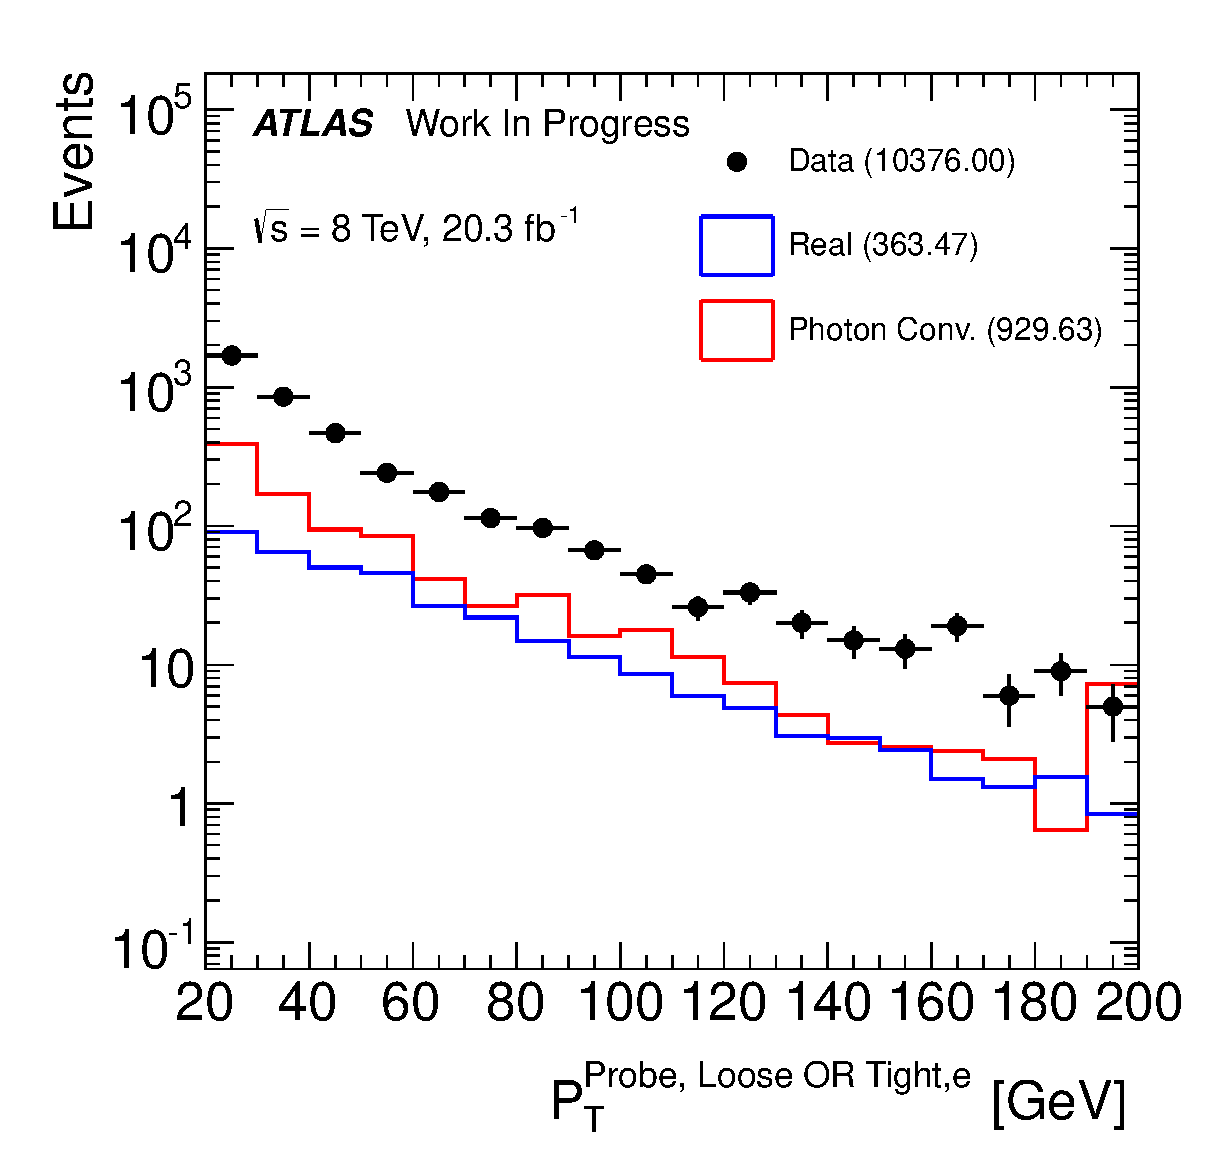
\includegraphics[width=0.45\columnwidth]{figures/fakes_bkg/CRs/SameSignElectronMuon/NoStack/ProbeLooseORTightElectronPt.eps}
}
%\centering
%\subfigure{
%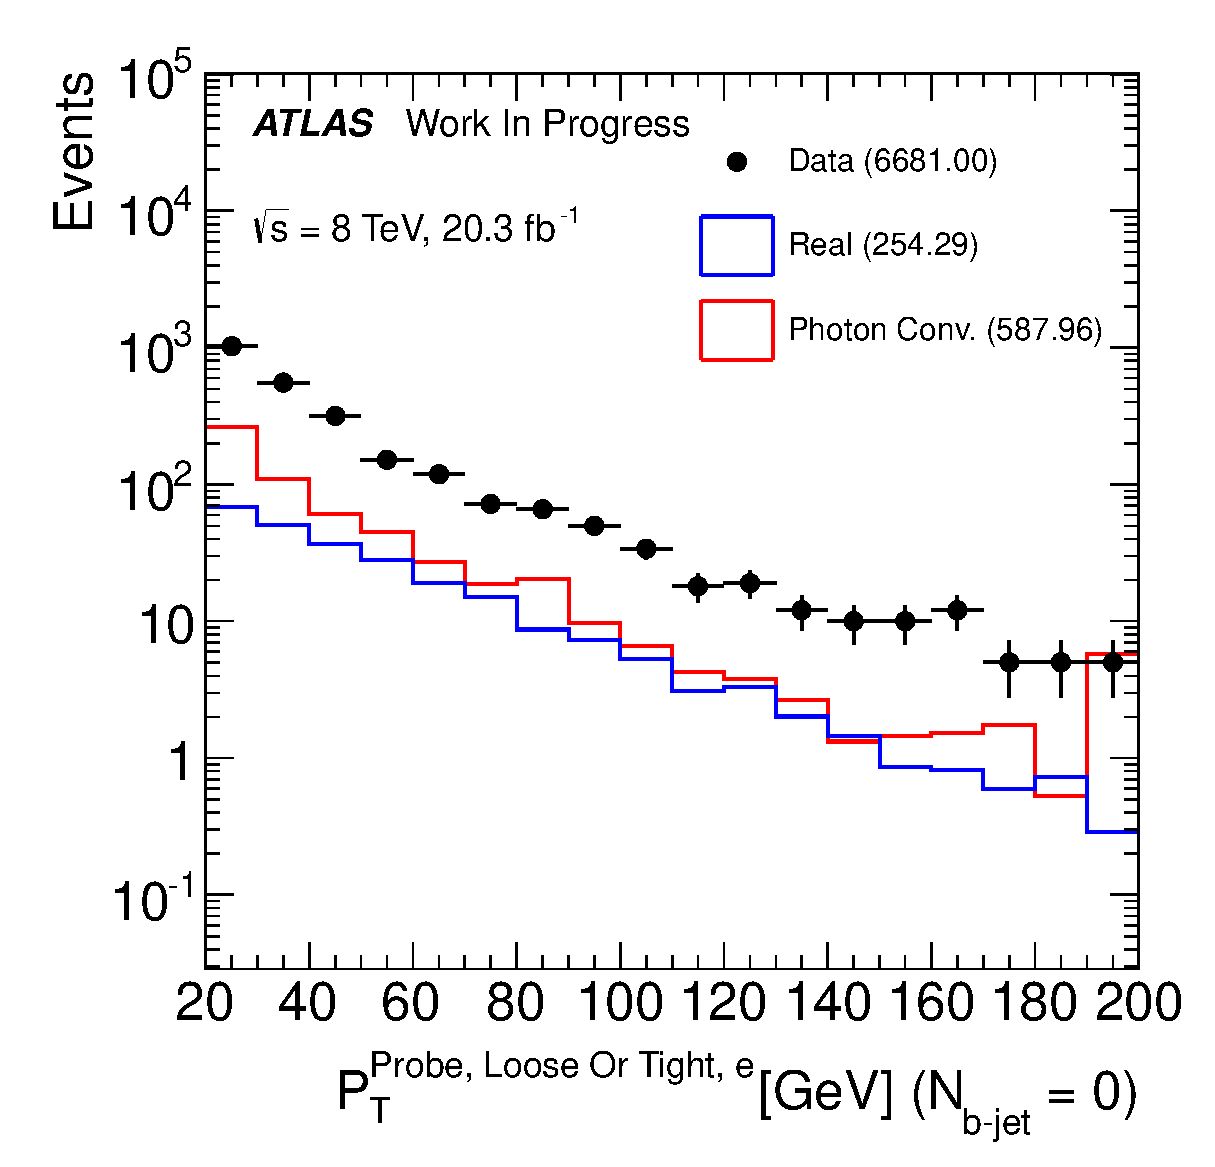
\includegraphics[width=0.3\columnwidth]{figures/fakes_bkg/CRs/SameSignElectronMuon/NoStack/ProbeLooseORTightElectronPtBJetEq0.eps}
%}
\centering
\subfigure{
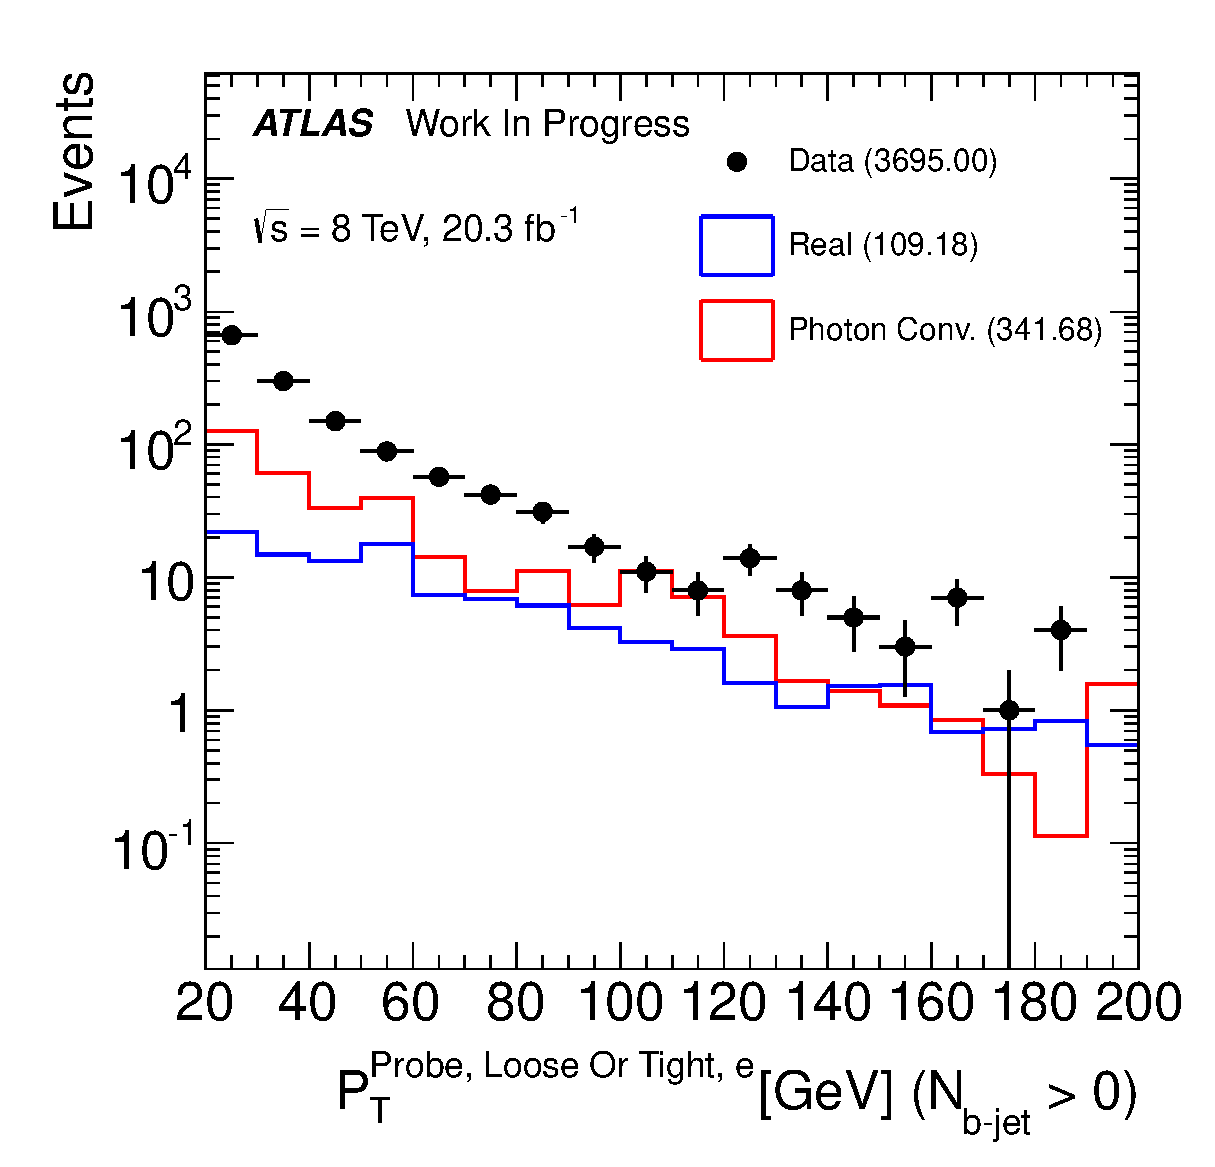
\includegraphics[width=0.45\columnwidth]{figures/fakes_bkg/CRs/SameSignElectronMuon/NoStack/ProbeLooseORTightElectronPtBJetGt0.eps}
}
%\vspace{-1mm}
\vspace{-10mm}\caption{Transverse momentum distributions \pt\ of tight probe electron (top) and loose or tight probe electrons (bottom) passing signal selection criteria in the Same-Sign $e-\mu$ control region without any additional requirement on $b$-jets in the event (left) and at least one $b$-jet (right).
The amount observed in data (black points) corresponds to $n$ (bottom) and $n_{\textrm{Tight}}$ (top) in Eq.~\ref{eq:fakerate}. 
Meanwhile, the contribution determined in MC to come from real leptons (blue line) and from photon conversion (red line) are shown 
separately; they are not stacked. The real lepton contribution corresponds to 
$n_{\textrm{Tight}}^{\textrm{Real}}$ (top) and $n^{\textrm{Real}}$ (bottom) and the photon conversion 
contribution corresponds to $n_{\textrm{Tight}}^{\textrm{PC}}$ (top) and $n^{\textrm{PC}}$ (bottom) in Eq.~\ref{eq:fakerate}.  }
\label{fig:fakeEff_CRs_electron}
\end{figure}






\begin{figure}[ht!]
\centering
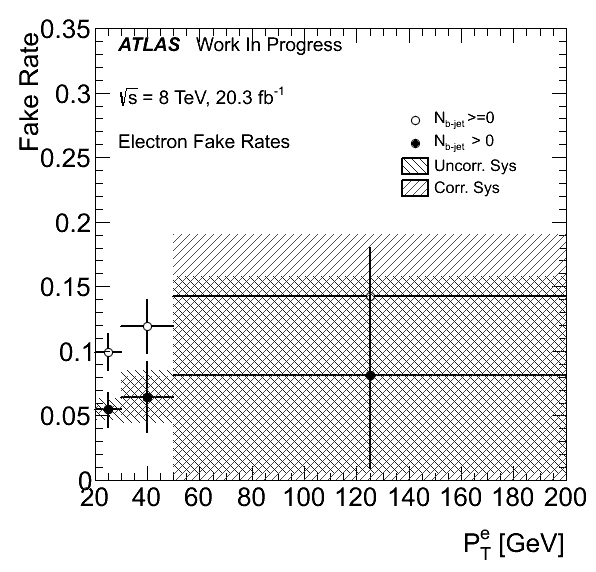
\includegraphics[width=0.45\columnwidth]{figures/fakes_bkg/Efficiencies/ElectronFakeRates.png}
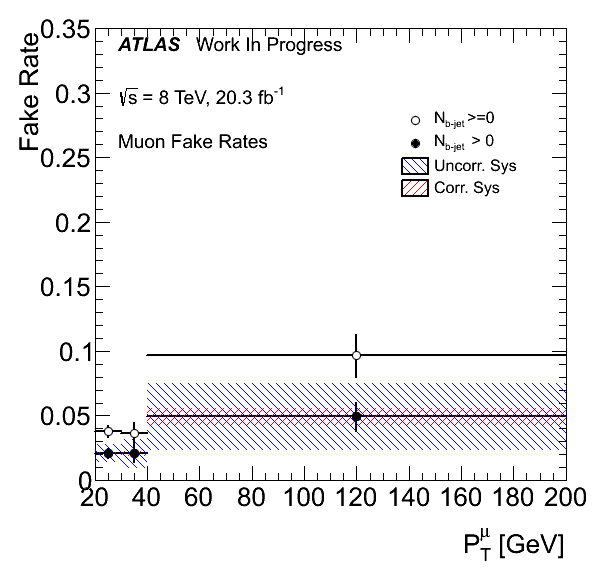
\includegraphics[width=0.45\columnwidth]{figures/fakes_bkg/Efficiencies/MuonFakeRates.png}
%\vspace{-10mm}
\caption{Distributions of the electron (left) and muon (right) fake rates as a function of \pt\ extracted in the control regions for three different selections: without any additional requirement on $b$-jets in the event and at least one $b$-jet.}
\label{fig:fakeEff}
\end{figure}




%\tabcolsep=0.1cm
%\begin{table}
%\centering
%\resizebox{0.8\textwidth}{!}{
%\begin{tabular}{l|c|c|c|c|c|c|c} 
%\hline
%\multicolumn{4}{c}{Electrons} &\multicolumn{4}{c}{Muons}\\ \hline
%\pt\ region & Fake eff. & $\sigma_{\mathrm{stat}}$ & $\sigma_{\mathrm{syst}}$ &\pt\ region & Fake eff. & $\sigma_{\mathrm{stat}}$ & $\sigma_{\mathrm{syst}}$ \\\hline
%$\pt \in [10, 15]$ \GeV\ & $0.$ & $0.$ & $0.$ 
%& $\pt \in [10, 15]$ \GeV\ & $0.$ & $0.$ & $0.$ \\
%$\pt \in [15, 30]$ \GeV\ & $0.$ & $0.$ & $0.$
%& $\pt \in [15, 20]$ \GeV\ & $0.$ & $0.$ & $0.$ \\
%$\pt\in [30, 50]$ \GeV\ & $0.$ & $0.$ & $0.$
%& $\pt\in [20, 40]$ \GeV\ & $0.$ & $0.$ & $0.$ \\
%$\pt > 50$ \GeV\ & $0.$ & $0.$ & $0.$
%& $\pt > 40$ \GeV\ & $0.$ & $0.$ & $0.$ \\
%\hline
%\end{tabular}  }
%\caption{Measured fake efficiencies for electrons and muons including statistical and systematic absolute uncertainties.} 
%\label{table:fakeEff_All}
%\end{table} 

\begin{table}[h]
\centering
\begin{tabular}{|l||c|c|c|c||c|c|c|c|}
\hline
 & $\zeta$ & $\sigma_{stat}$ & $\sigma_{sys}^{uncorr}$ & $\sigma_{sys}^{corr}$\\ 
\hline\hline
&\multicolumn{4}{c||}{$N_{b-jet} > 0$}\\ \hline
$p_{T}\in[20,30]$ GeV &  $0.0549$ &  $0.0136$ &  $0.0084$ &  $0.0032$\\ 
$p_{T}\in[30,50]$ GeV &  $0.0645$ &  $0.0272$ &  $0.0203$ &  $0.0161$\\ 
$p_{T} > 50$ GeV &  $0.0816$ &  $0.0723$ &  $0.0764$ &  $0.1088$\\ 
\hline\hline &\multicolumn{4}{c||}{$N_{b-jet} \geq 0$}\\ \hline
$p_{T}\in[20,30]$ GeV &  $0.0995$ &  $0.0141$ &  $0.0270$ &  $0.0099$\\ 
$p_{T}\in[30,50]$ GeV &  $0.1192$ &  $0.0208$ &  $0.0324$ &  $0.0232$\\ 
$p_{T} > 50$ GeV &  $0.1428$ &  $0.0374$ &  $0.0428$ &  $0.0674$\\ 
\hline
\end{tabular}

\caption{Measured fake efficiencies for electrons measured in three regions: with no additional requirements on the presence of $b$-jets and with at least one $b$-jet in a event. Statistical and systematic absolute uncertainties are also shown.} 
\label{table:fakeEff_El}
\end{table} 


\begin{table}[h]
\centering
\begin{tabular}{|l||c|c|c|c||c|c|c|c|}
\hline
 & $\zeta$ & $\sigma_{stat}$ & $\sigma_{sys}^{uncorr}$ & $\sigma_{sys}^{corr}$\\ 
\hline\hline
&\multicolumn{4}{c||}{$N_{b-jet} > 0$}\\ \hline
$p_{T}\in[20,30]$ GeV &  $0.0208$ &  $0.0037$ &  $0.0067$ &  $0.0009$\\ 
$p_{T}\in[30,40]$ GeV &  $0.0207$ &  $0.0066$ &  $0.0113$ &  $0.0020$\\ 
$p_{T} > 40$ GeV &  $0.0492$ &  $0.0109$ &  $0.0259$ &  $0.0068$\\ 
\hline\hline &\multicolumn{4}{c||}{$N_{b-jet} \geq 0$}\\ \hline
$p_{T}\in[20,30]$ GeV &  $0.0378$ &  $0.0046$ &  $0.0140$ &  $0.0040$\\ 
$p_{T}\in[30,40]$ GeV &  $0.0360$ &  $0.0091$ &  $0.0096$ &  $0.0089$\\ 
$p_{T} > 40$ GeV &  $0.0967$ &  $0.0166$ &  $0.0252$ &  $0.0244$\\ 
\hline
\end{tabular}

\caption{Measured fake efficiencies for muons measured in three regions: with no additional requirements on the presence of $b$-jets and with at least one $b$-jet in the event.  Statistical and systematic absolute uncertainties are also shown.} 
\label{table:fakeEff_Mu}
\end{table} 


\clearpage

\subsubsection{Study of the fake lepton composition}
\label{sec:fakecomposition}

The use of the generalized matrix method to determine the 
relies on the assumption that the 
fake rates derived in the di-lepton control regions may be extrapolated to the three lepton signal regions.  
The fake rate depends primarily on the source of the fake leptons, thus
one can check the validity of this assumption by looking at the composition of the
different fake lepton sources in the dilepton control regions and comparing 
them to the
composition in the three lepton signal regions. 

The fake composition is investigated by classifying the MC events as a function of the origin of the fake leptons found in each event.  The MCTruthClassifier tool~\cite{MCtruthclassifier:twiki} is used
to identify the fake laptops origin as follows:

\begin{itemize}
\item Real - Prompt leptons
		\begin{itemize}
		\item \emph{IsoElectron} 
		\item \emph{IsoMuon}
		\item In $Z\gamma$ events classified as either \emph{UnknownElectron} or \emph{UnknownMuon} and parent of lepton is $\gamma$.
		\item In $Z\rightarrow\tau\tau$ events classified as either \emph{NonIsoElectron} or \emph{NonIsoMuon} and lepton has $\tau$ as parent.
		\end{itemize}
\item Heavy Flavor (HF) - Leptons from heavy flavor jets or heavy hadron decays
		\begin{itemize}
		\item \emph{NonIsoElectron} 
		\item \emph{NonIsoMuon}
		\end{itemize}
\item Light Flavor (LF) -  Leptons from light flavor jets
		\begin{itemize}
		\item \emph{Hadron} 
		\item \emph{Others}
		\item In $ZWW$ and $ZZZ$ events classified as either \emph{UnknownElectron} or \emph{UnknownMuon} and parent of lepton is either an up quark, down quark, or a gluon.
		\end{itemize}
\item Photon Conversion (PC)  - Leptons due to radiation
		\begin{itemize}
		\item \emph{BkgElectron} 
		\item \emph{BkgMuon}
		\end{itemize}

\end{itemize}

The composition is shown for electrons in the dilepton control 
regions in Table~\ref{table:CompositionElectronCR} and in the event pre-selection and in region close to the signal regions in Table~\ref{table:CompositionElectronSR}.
First, one can see that the PC contribution is roughly half of the fake contribution
estimate using MC
in the control regions and in the region close to the signal regions. Since this is being estimated
using MC close to the signal regions, 
this component is subtracted out in order to remove any double counting
in the final estimate. Then, after subtraction,
if one compares the composition in the control regions
to the composition in the region close to the signal regions only for electrons, 
in particular after tight selection, one can see that 
the composition is similar for both, 
with about 50 to 75 \% coming from HF and the rest from LF.

For the muons, one can see the composition in the dilepton control regions in 
Table~\ref{table:CompositionMuonCR} and in the event pre-selection
and region close to the signal regions in Table~\ref{table:CompositionMuonSR}. For the muons the PC
component is negligible, as expected, and there is no need for subtraction.
In this case, the composition is dominated by HF, contributing about 90\% with the
rest coming from LF.  This is true in the region close to the signal regions and in the control regions.

The differences observed in the composition between the inclusive $b-jet$ and $b-jet$ 
tagged dilepton control regions is observed to be of a similar size
to the difference in the composition for the region close to the signal regions for both the electron 
and muon cases.
Thus, comparing the rates derived in the control regions using the two different
$b-jet$ criteria should take into account any differences in the composition due
to extrapolation. This is the motivation for choosing the difference in these two 
control regions as an additional systematic on the fake rates.

Using this study of the composition, we conclude that the composition appears to be
consistent between the control regions and the region close to the signal regions.  We have chosen 
a comparison of two different dilepton control regions to be used a systematic
which should take into account any remaining differences in the composition.

It should be said that in the dilepton control regions, 
the MC estimate strongly underestimates the amount observed
in data, presumably because of additional sources of fakes 
not modeled in our MC, such as from QCD. 
The difference in the estimates can be clearly seen in Figures~\ref{fig:fakeEff_CRs_muon_stacked}
and \ref{fig:fakeEff_CRs_electron_stacked} which show the stacked MC estimate from real, photon conversion,
heavy flavor and light flavor sources compared to data.
Thus, the composition estimates shown are only reliable 
if these additional sources would have a similar composition to the ones observed
in this study that we are able to model. This effectively 
puts a large uncertainty on the composition estimates observed in this study. Also,
because the additinonal sources are most likely dominated by QCD, the PC 
contribution to these sources should be small. Thus, the PC component before subtraction
is likely overstated as shown in 
Tables~\ref{table:CompositionElectronCR} 
and \ref{table:CompositionElectronSR}.
As discussed earlier, we subtract the PC
component from the data when obtaining the fake rate. This procedure then assumes
explicitly that all of the photon conversion contribution is modeled in MC and is 
small.


\begin{figure}[h!]
\centering
\subfigure{
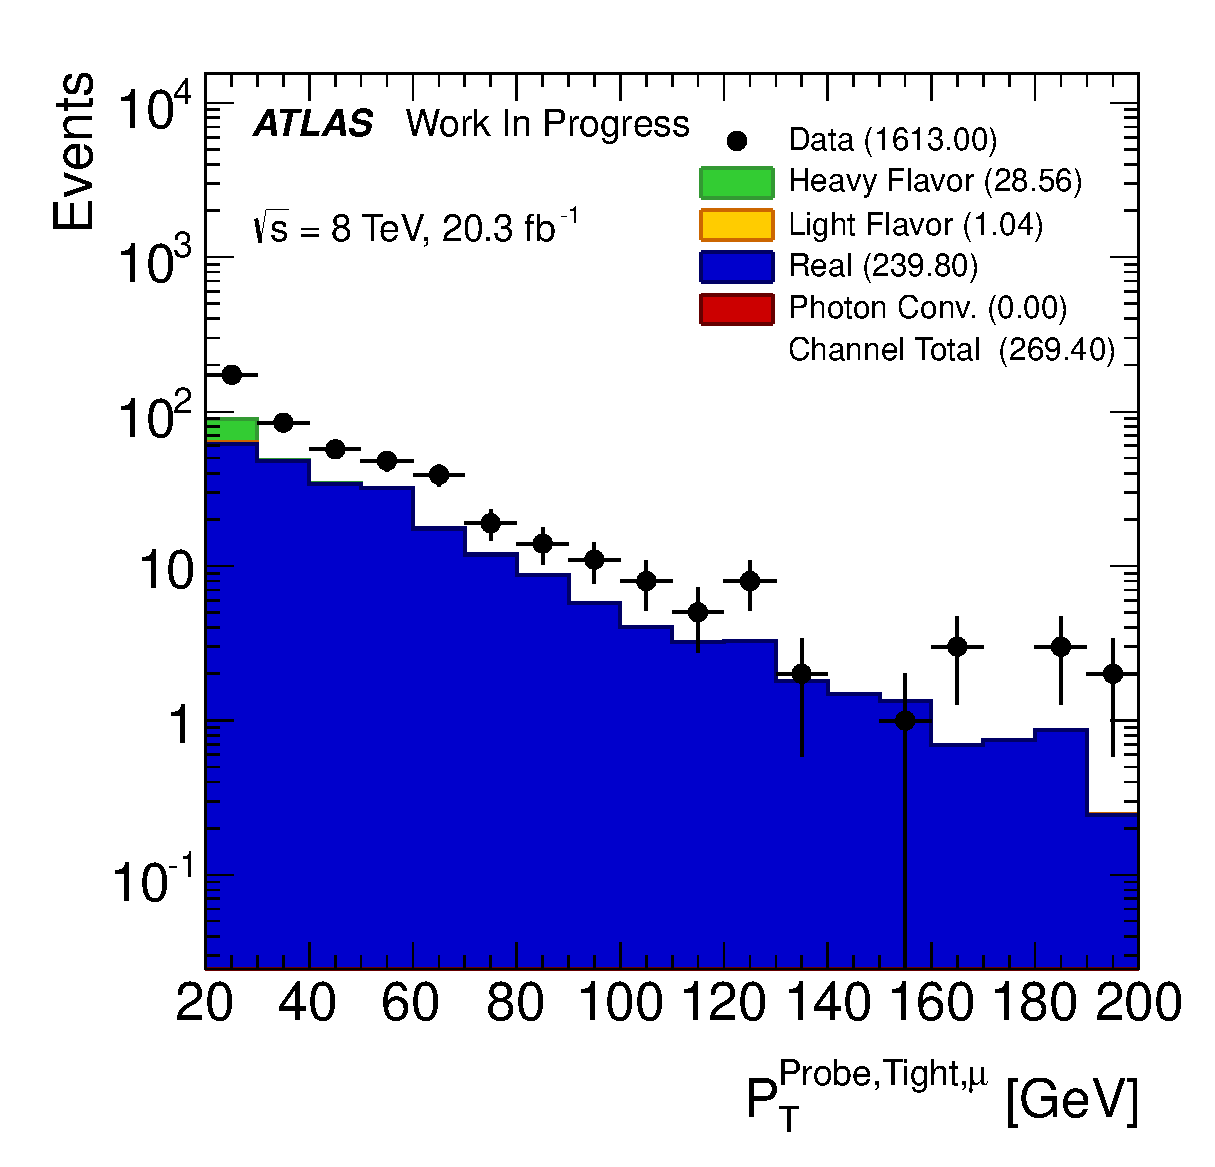
\includegraphics[width=0.45\columnwidth]{figures/fakes_bkg/CRs/SameSignMuonMuon/Stacked/ProbeTightMuonPt.eps}
}
%\centering
%\subfigure{
%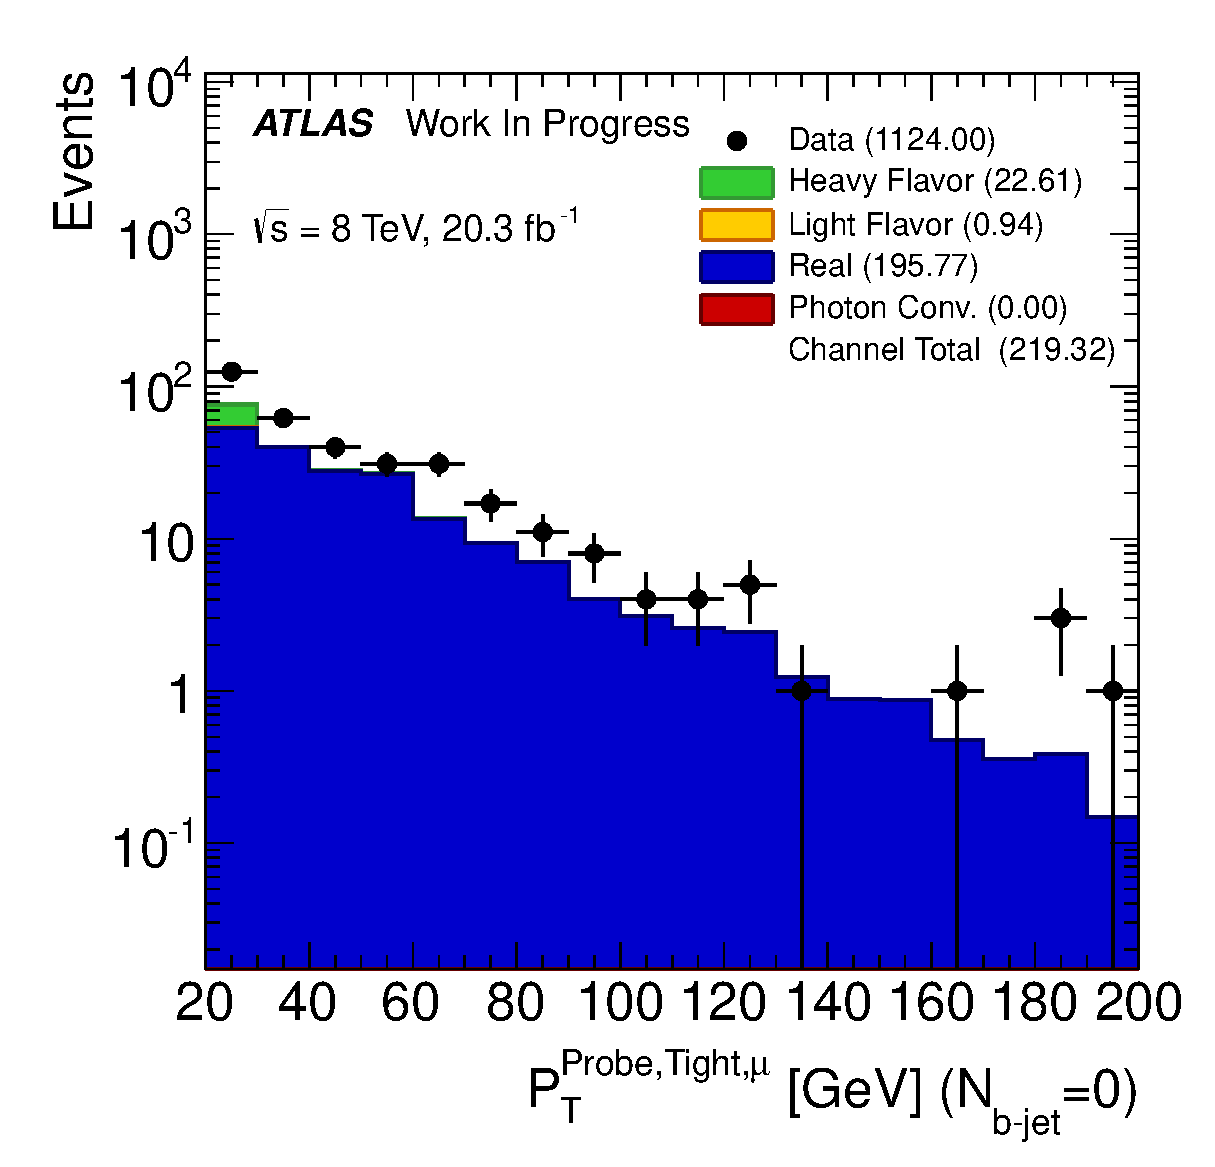
\includegraphics[width=0.3\columnwidth]{figures/fakes_bkg/CRs/SameSignMuonMuon/Stacked/ProbeTightMuonPtBJetEq0.eps}
%}
\centering
\subfigure{
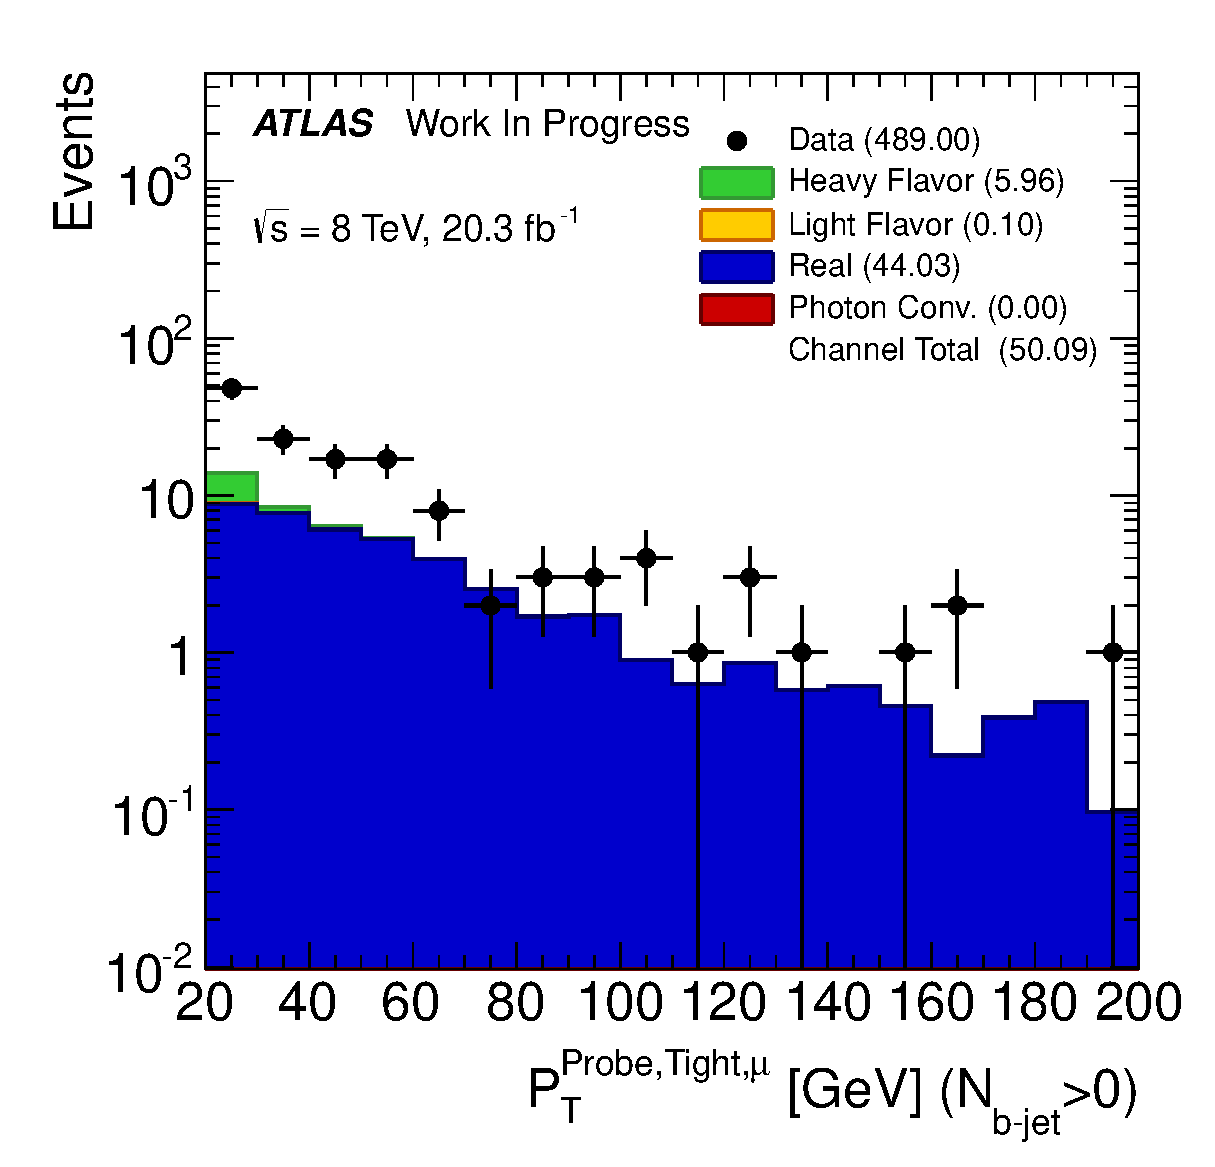
\includegraphics[width=0.45\columnwidth]{figures/fakes_bkg/CRs/SameSignMuonMuon/Stacked/ProbeTightMuonPtBJetGt0.eps}
}
%\vspace{-1mm}
\centering
\subfigure{
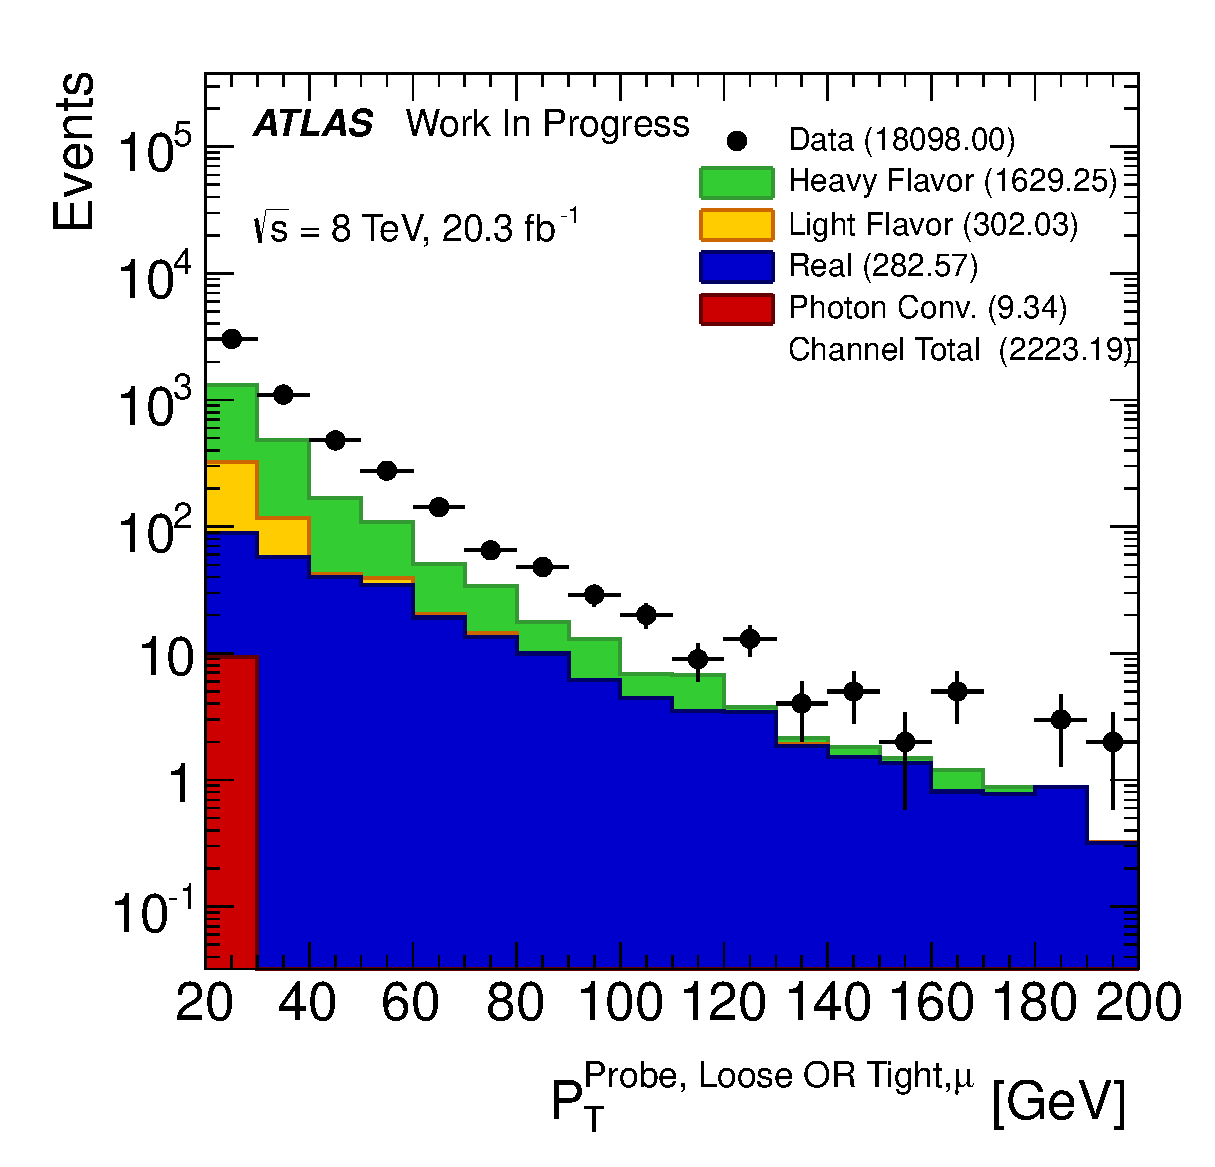
\includegraphics[width=0.45\columnwidth]{figures/fakes_bkg/CRs/SameSignMuonMuon/Stacked/ProbeLooseORTightMuonPt.eps}
}
%\centering
%\subfigure{
%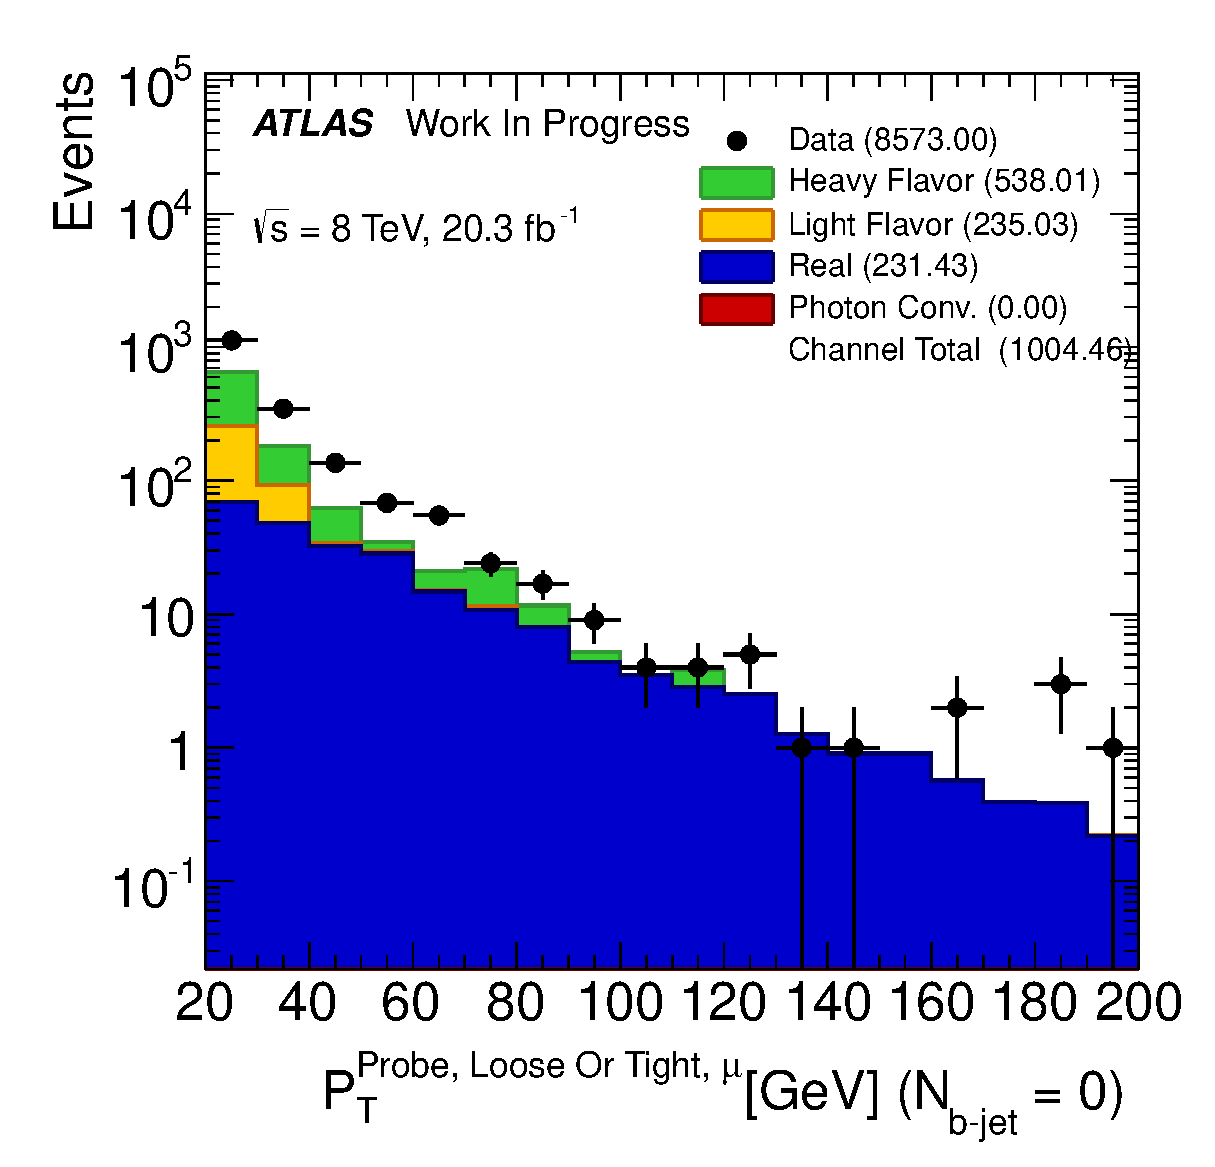
\includegraphics[width=0.45\columnwidth]{figures/fakes_bkg/CRs/SameSignMuonMuon/Stacked/ProbeLooseORTightMuonPtBJetEq0.eps}
%}
\centering
\subfigure{
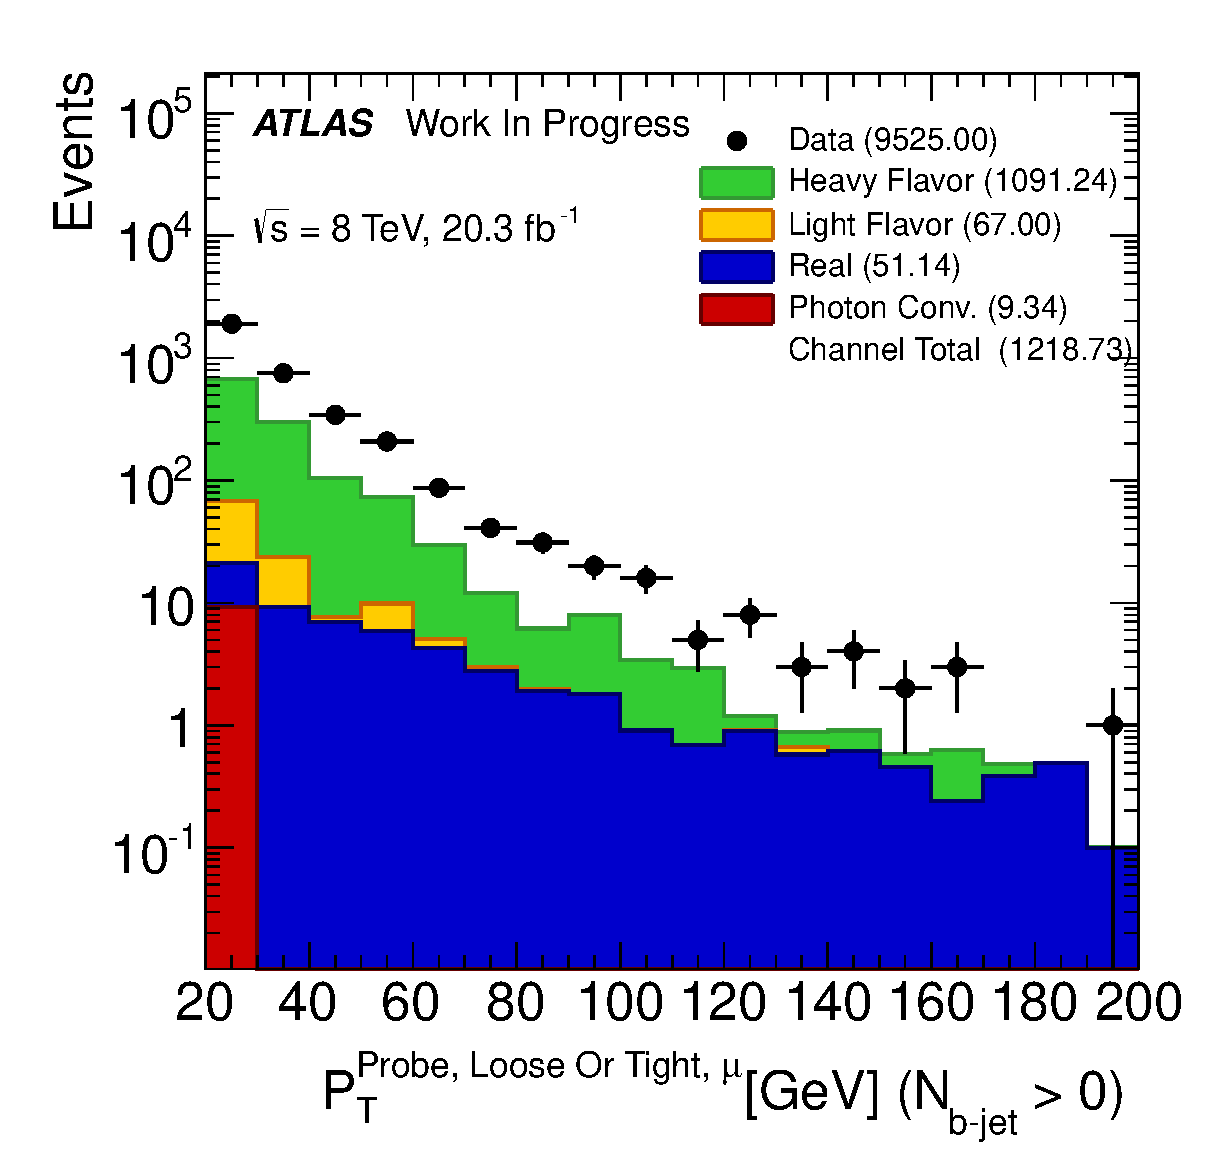
\includegraphics[width=0.45\columnwidth]{figures/fakes_bkg/CRs/SameSignMuonMuon/Stacked/ProbeLooseORTightMuonPtBJetGt0.eps}
}
\vspace{-10mm}\caption{Transverse momentum distributions \pt\ of tight probe muons (top) and loose OR tight probe muons (bottom) passing signal selection criteria in the control Same-Sign $\mu-\mu$ control region without any additional requirement on $b$-jets in the event (left) and at least one $b$-jet (right). 
The amount observed in data (black points) corresponds to $n$ (bottom) and $n_{\textrm{Tight}}$ (top) in Eq.~\ref{eq:fakerate}. 
Meanwhile, the contribution determined in MC to come from real leptons (blue), photon conversion (red), heavy flavor (green) and light
flavor (orange) are shown stacked on top of each other. 
The difference between the data and MC does not effect the data-driven
fake estimate but may have an impact on the composition estiamte.
}
\label{fig:fakeEff_CRs_muon_stacked}
\end{figure}

\begin{figure}[h!]
\centering
\subfigure{
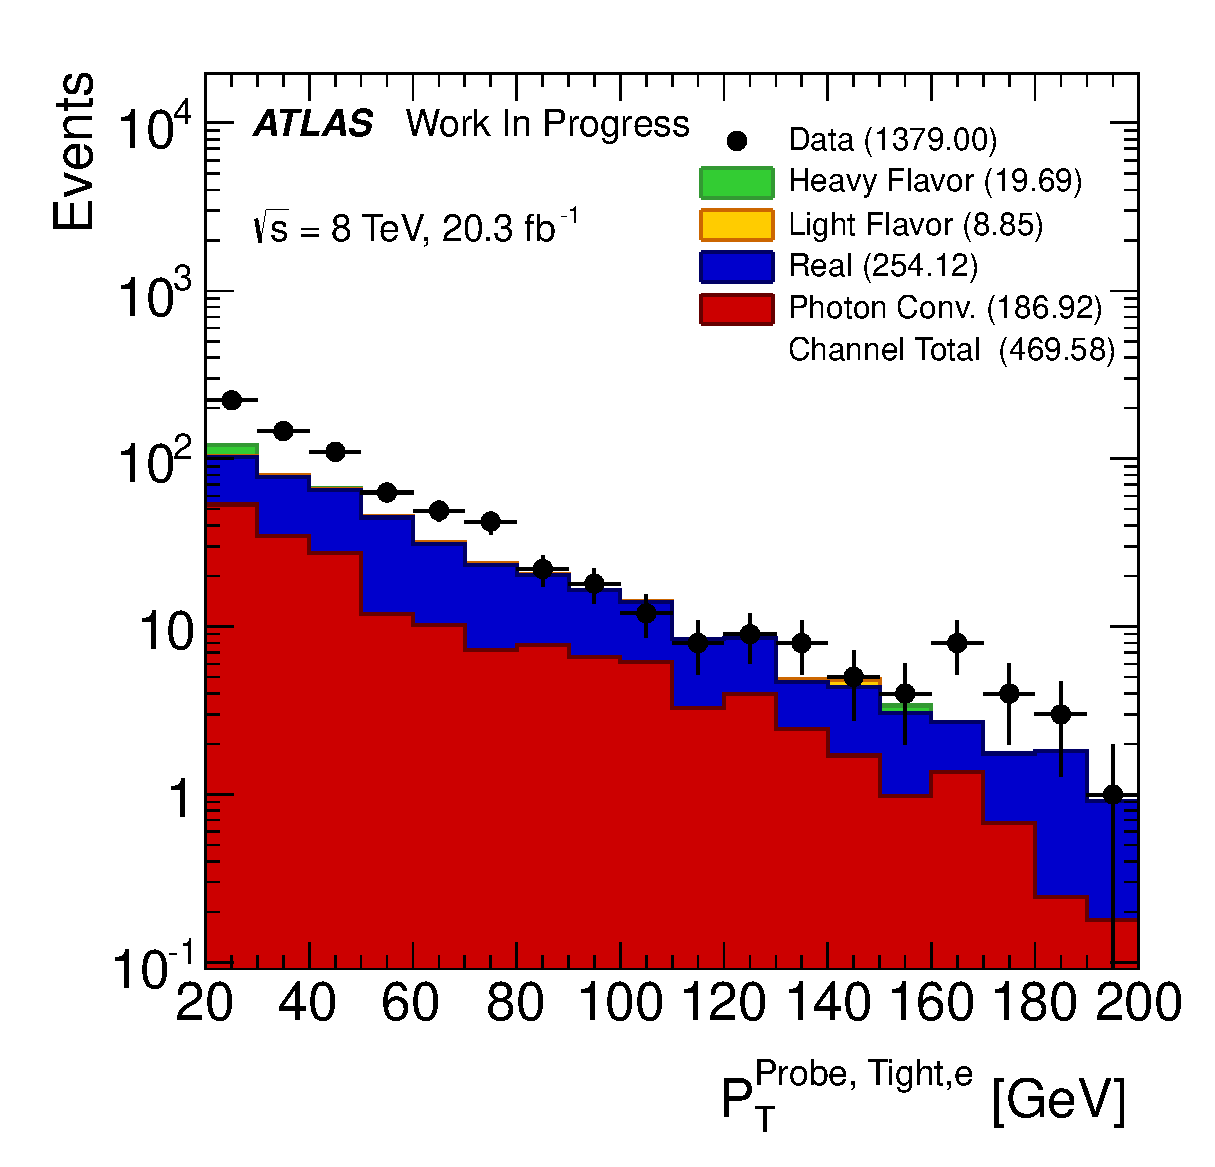
\includegraphics[width=0.45\columnwidth]{figures/fakes_bkg/CRs/SameSignElectronMuon/Stacked/ProbeTightElectronPt.eps}
}
%\centering
%\subfigure{
%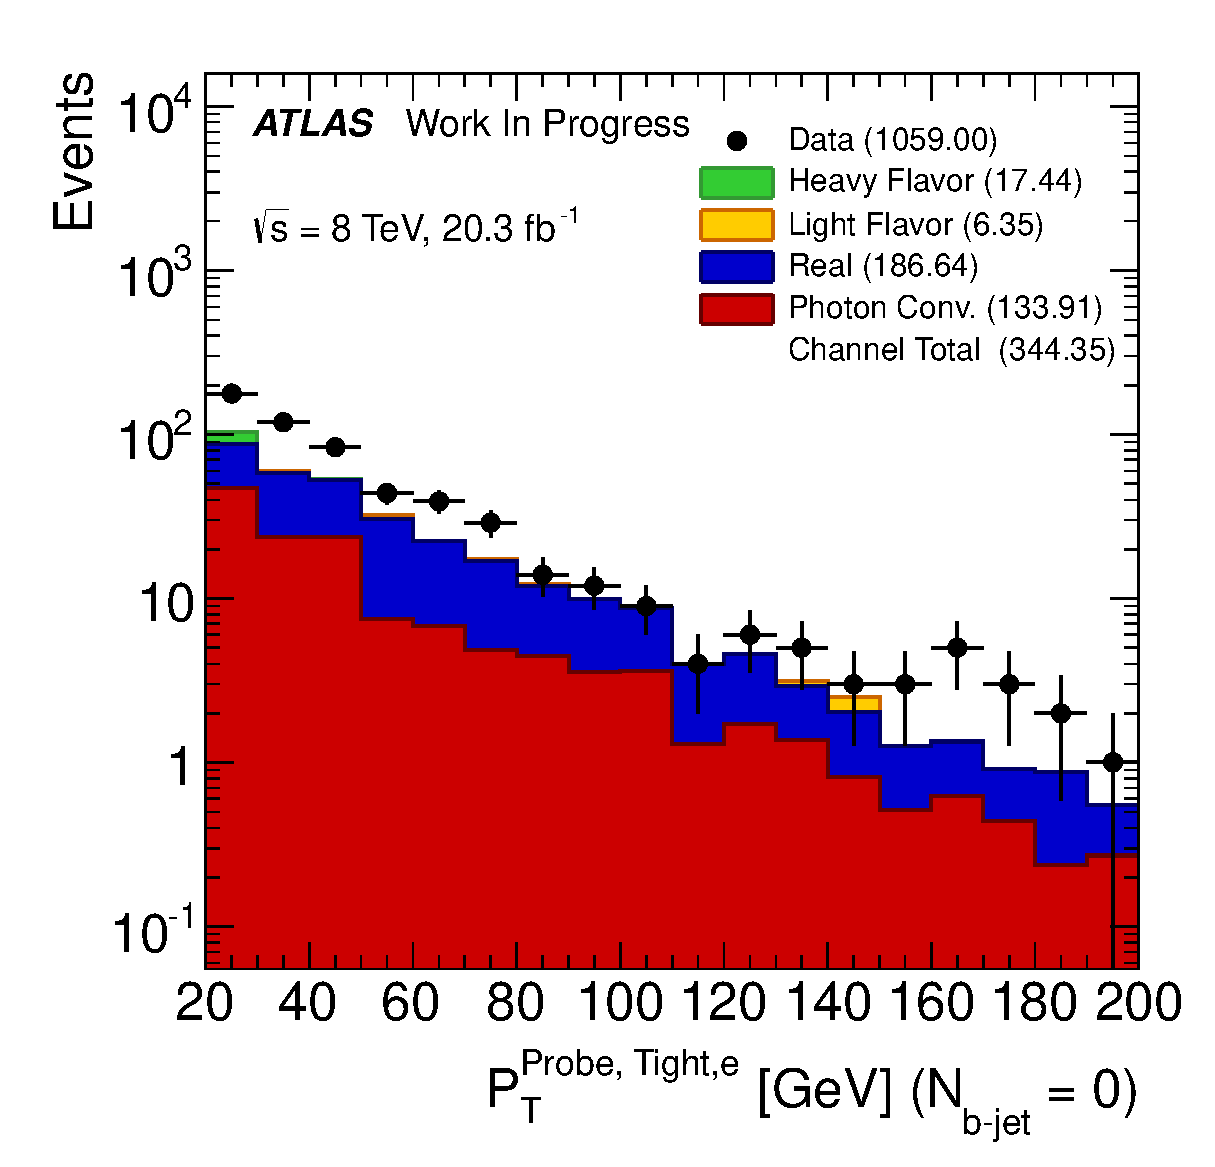
\includegraphics[width=0.3\columnwidth]{figures/fakes_bkg/CRs/SameSignElectronMuon/Stacked/ProbeTightElectronPtBJetEq0.eps}
%}
\centering
\subfigure{
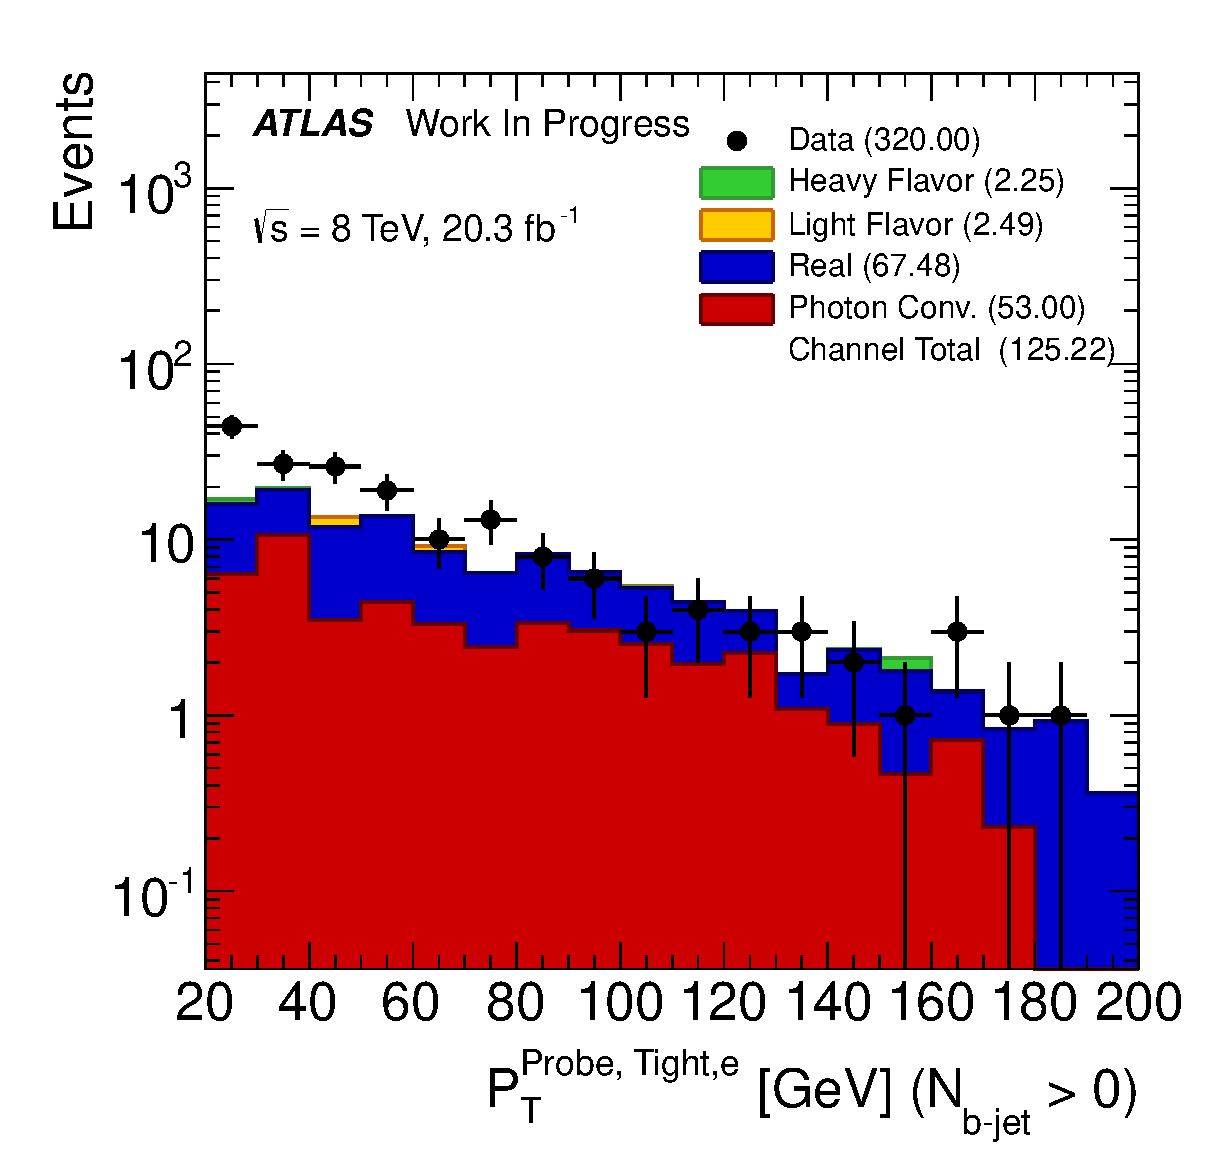
\includegraphics[width=0.45\columnwidth]{figures/fakes_bkg/CRs/SameSignElectronMuon/Stacked/ProbeTightElectronPtBJetGt0.eps}
}
\centering
\subfigure{
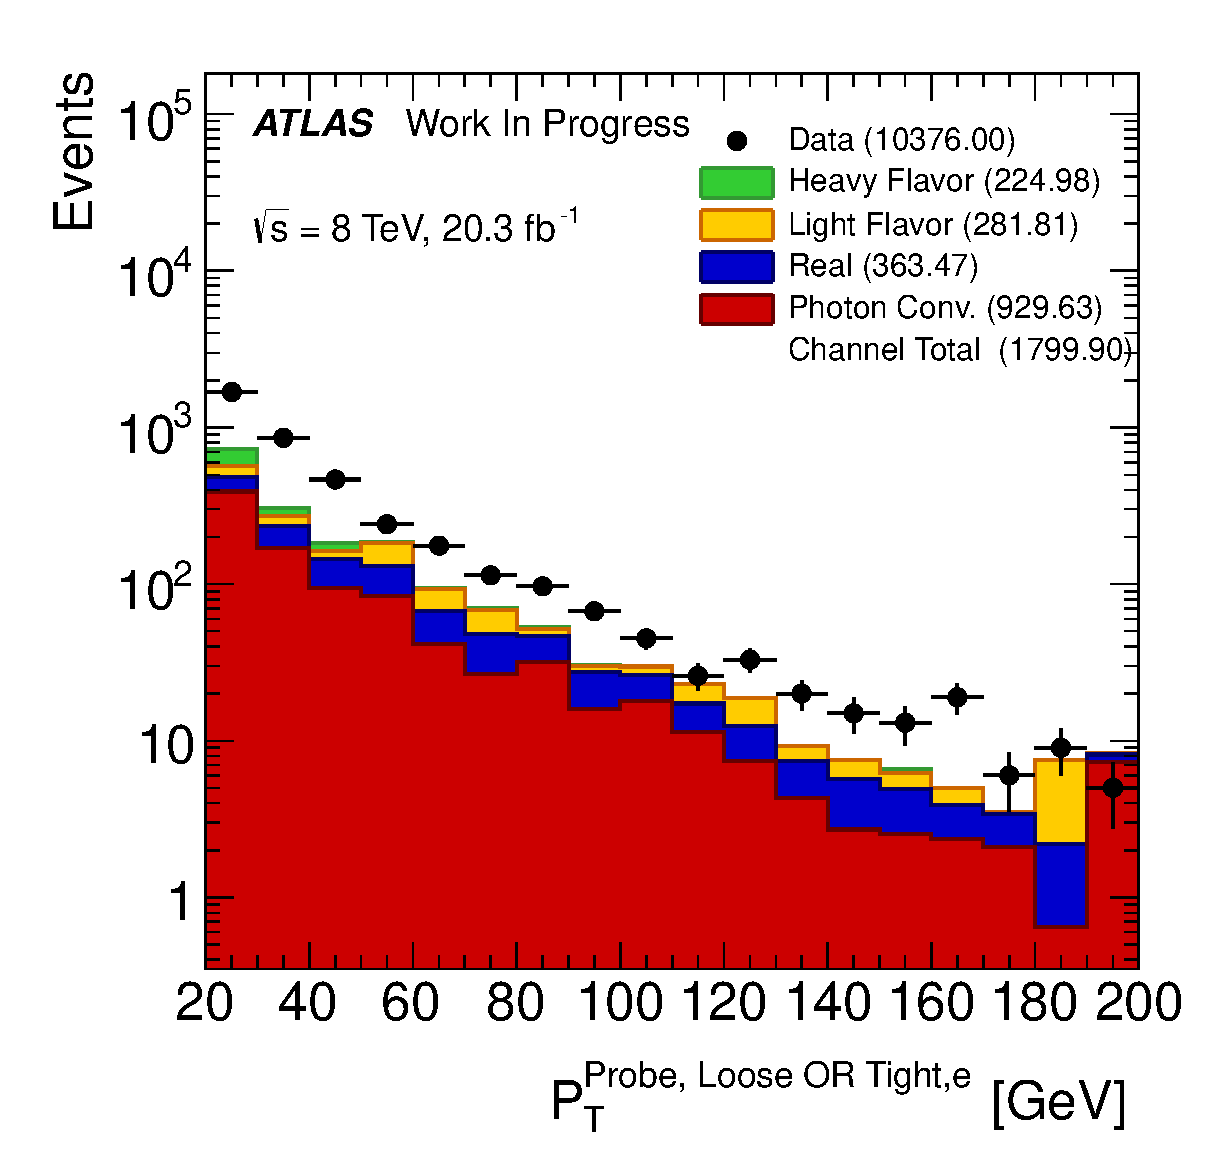
\includegraphics[width=0.45\columnwidth]{figures/fakes_bkg/CRs/SameSignElectronMuon/Stacked/ProbeLooseORTightElectronPt.eps}
}
%\centering
%\subfigure{
%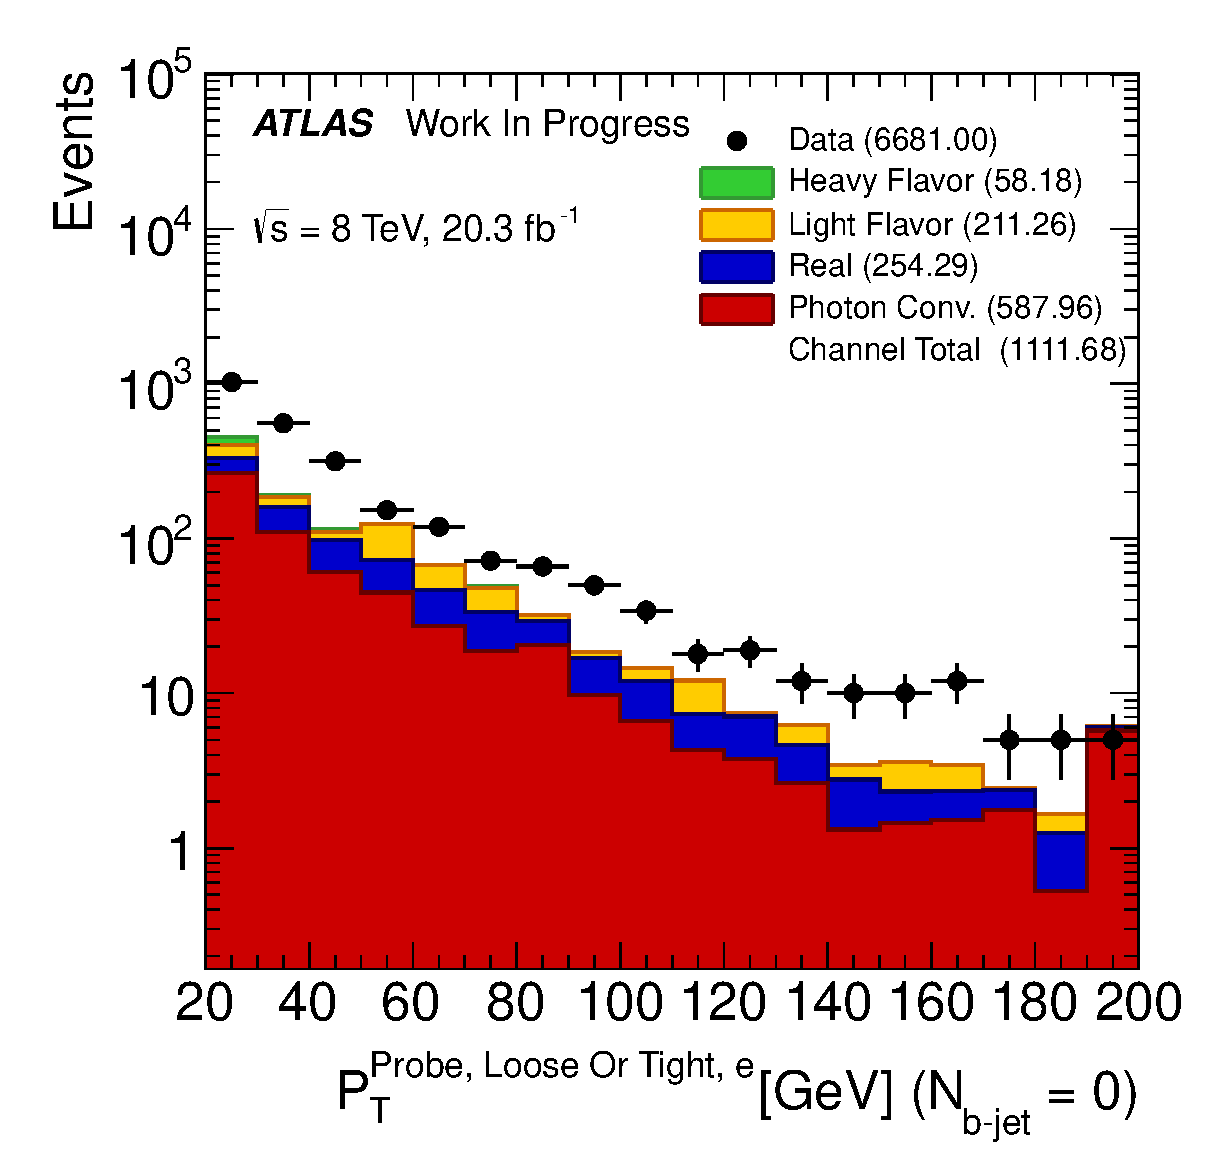
\includegraphics[width=0.3\columnwidth]{figures/fakes_bkg/CRs/SameSignElectronMuon/Stacked/ProbeLooseORTightElectronPtBJetEq0.eps}
%}
\centering
\subfigure{
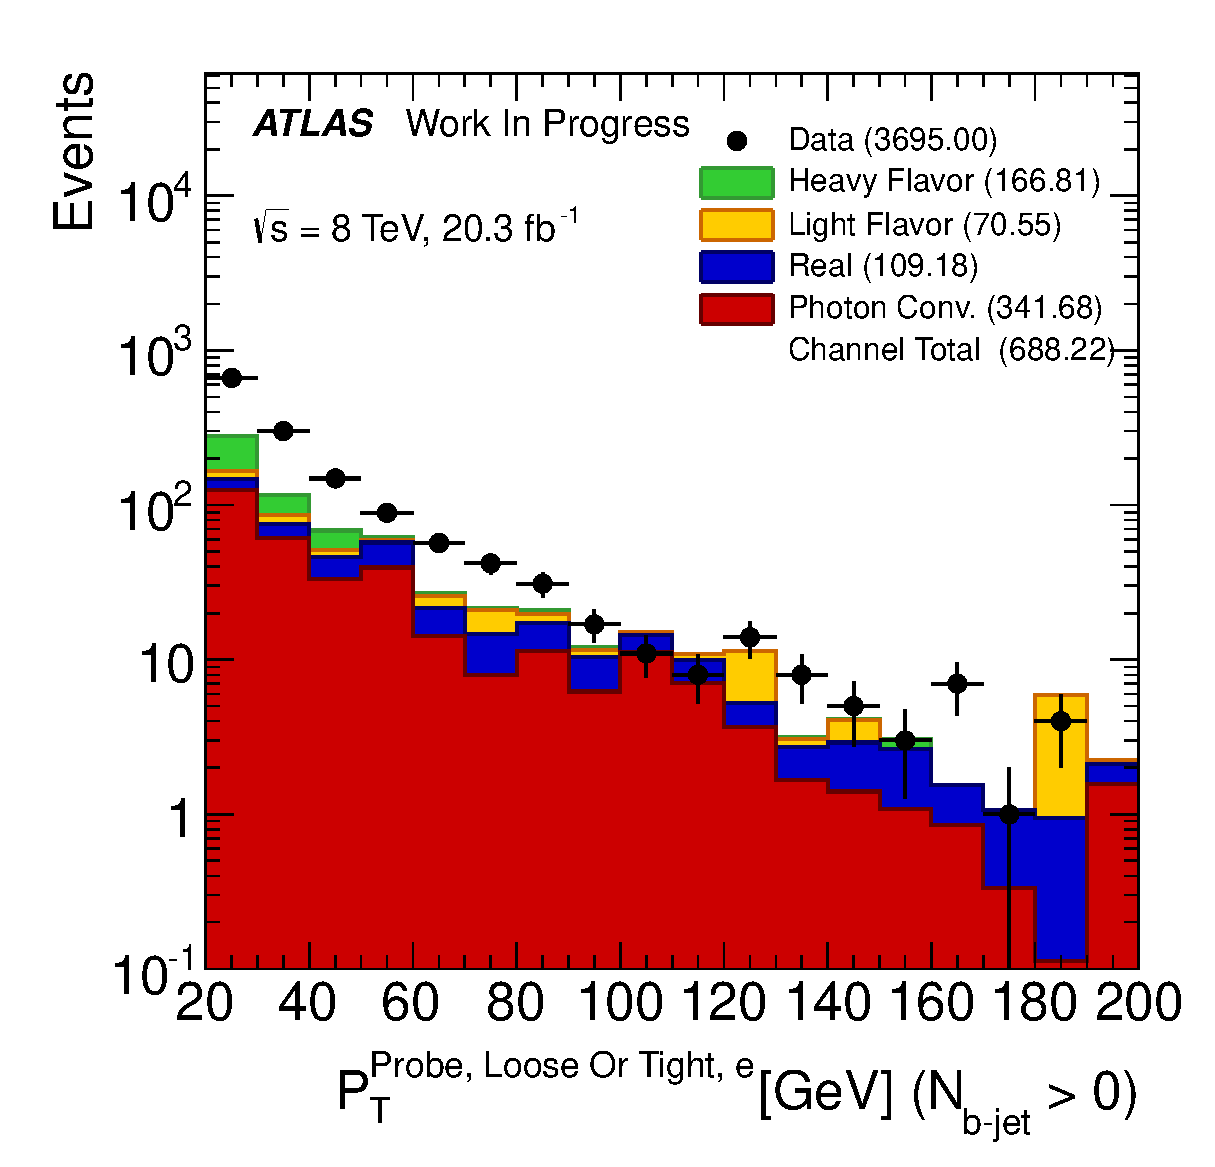
\includegraphics[width=0.45\columnwidth]{figures/fakes_bkg/CRs/SameSignElectronMuon/Stacked/ProbeLooseORTightElectronPtBJetGt0.eps}
}
%\vspace{-1mm}
\vspace{-10mm}\caption{Transverse momentum distributions \pt\ of tight probe electron (top) and loose or tight probe electrons (bottom) passing signal selection criteria in the Same-Sign $e-\mu$ control region without any additional requirement on $b$-jets in the event (left) and at least one $b$-jet (right).
The amount observed in data (black points) corresponds to $n$ (bottom) and $n_{\textrm{Tight}}$ (top) in Eq.~\ref{eq:fakerate}. 
Meanwhile, the contribution determined in MC to come from real leptons (blue), photon conversion (red), heavy flavor (green) and light
flavor (orange) are shown stacked on top of each other.
The difference between the data and MC does not effect the data-driven
fake estimate but may have an impact on the composition estiamte.
}
\label{fig:fakeEff_CRs_electron_stacked}
\end{figure}

%%%%%%%%%%%scaled

%\begin{figure}[h!]
%\centering
%\subfigure{
%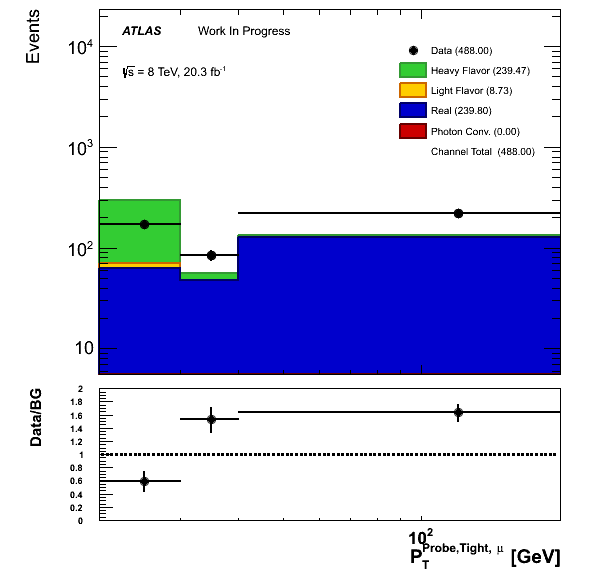
\includegraphics[width=0.45\columnwidth]{figures/fakes_bkg/CRs/SameSignMuonMuon/Scaled/coarse/ProbeTightMuonPtFakeRate_histratio.png}
%}
%\centering
%\subfigure{
%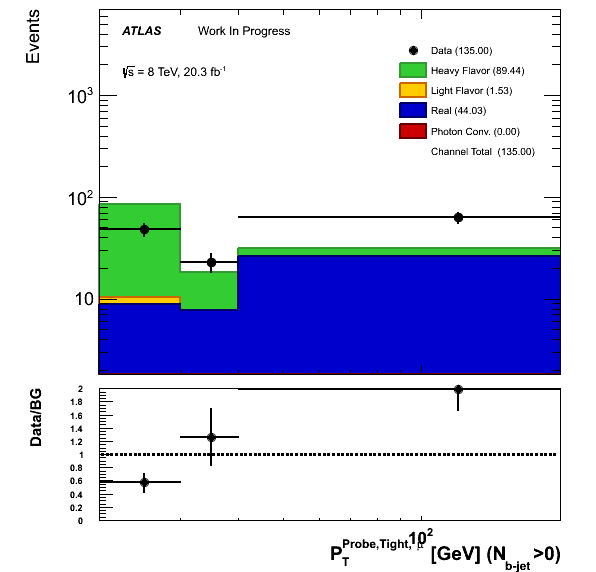
\includegraphics[width=0.45\columnwidth]{figures/fakes_bkg/CRs/SameSignMuonMuon/Scaled/coarse/ProbeTightMuonPtBJetGt0FakeRate_histratio.png}
%}
%\centering
%\subfigure{
%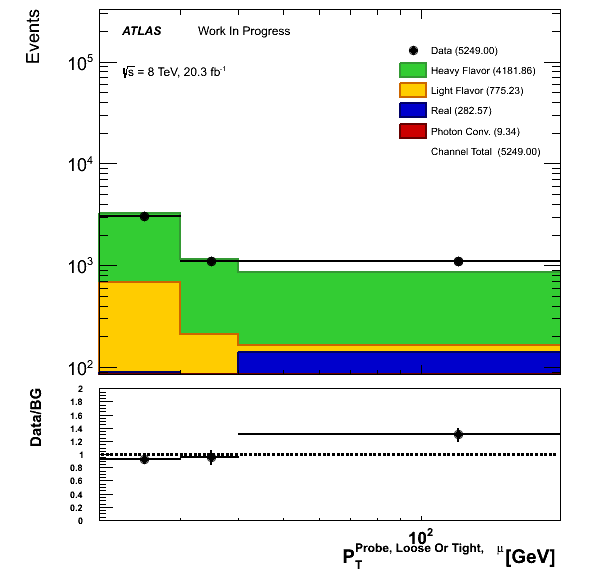
\includegraphics[width=0.45\columnwidth]{figures/fakes_bkg/CRs/SameSignMuonMuon/Scaled/coarse/ProbeLooseORTightMuonPtFakeRate_histratio.png}
%}
%\centering
%\subfigure{
%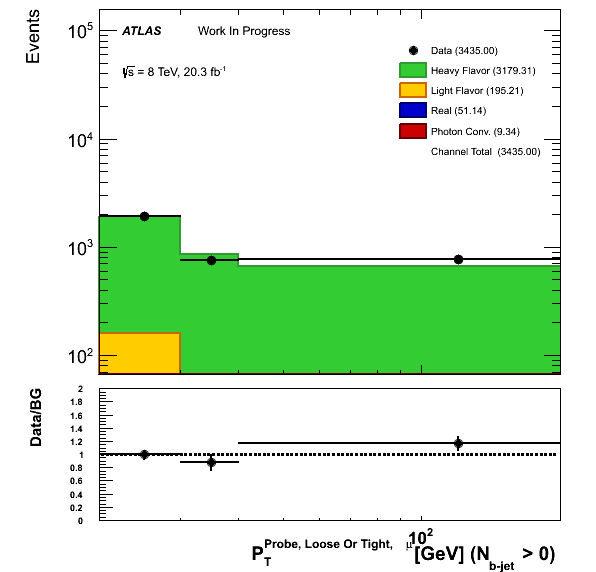
\includegraphics[width=0.45\columnwidth]{figures/fakes_bkg/CRs/SameSignMuonMuon/Scaled/coarse/ProbeLooseORTightMuonPtBJetGt0FakeRate_histratio.png}
%}
%\vspace{-10mm}\caption{Scaled....Transverse momentum distributions \pt\ of tight probe muons (top) and loose OR tight probe muons (bottom) passing signal selection criteria in the control Same-Sign $\mu-\mu$ control region without any additional requirement on $b$-jets in the event (left) and at least one $b$-jet (right). 
%The amount observed in data (black points) corresponds to $n$ (bottom) and $n_{\textrm{Tight}}$ (top) in Eq.~\ref{eq:fakerate}. 
%Meanwhile, the contribution determined in MC to come from real leptons (blue), photon conversion (red), heavy flavor (green) and light
%flavor (orange) are shown stacked on top of each other. 
%The difference between the data and MC does not effect the data-driven
%fake estimate but may have an impact on the composition estiamte.
%}
%\label{fig:fakeEff_CRs_muon_stacked_scaled}
%\end{figure}

%\begin{figure}[h!]
%\centering
%\subfigure{
%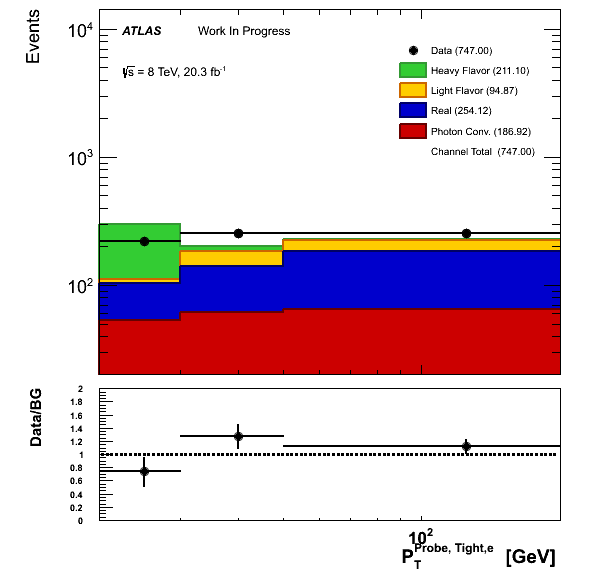
\includegraphics[width=0.45\columnwidth]{figures/fakes_bkg/CRs/SameSignElectronMuon/Scaled/coarse/ProbeTightElectronPtFakeRate_histratio.png}
%}
%\centering
%\subfigure{
%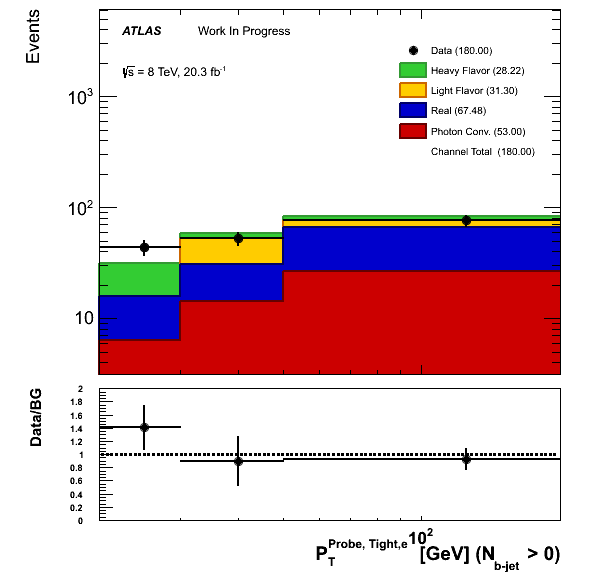
\includegraphics[width=0.45\columnwidth]{figures/fakes_bkg/CRs/SameSignElectronMuon/Scaled/coarse/ProbeTightElectronPtBJetGt0FakeRate_histratio.png}
%}
%\centering
%\subfigure{
%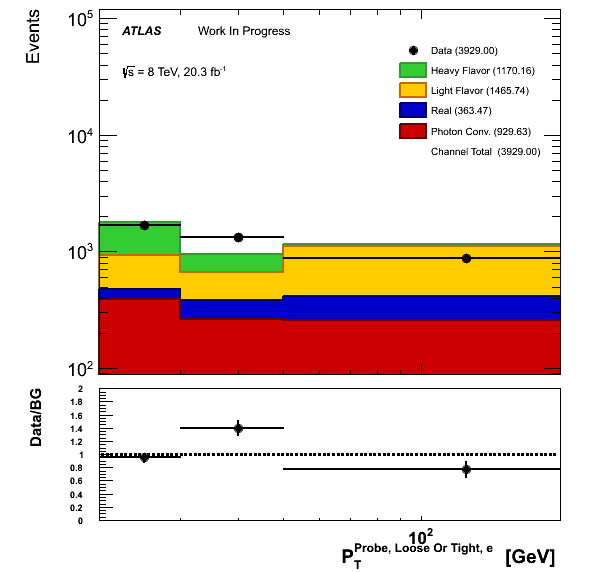
\includegraphics[width=0.45\columnwidth]{figures/fakes_bkg/CRs/SameSignElectronMuon/Scaled/coarse/ProbeLooseORTightElectronPtFakeRate_histratio.png}
%}
%\centering
%\subfigure{
%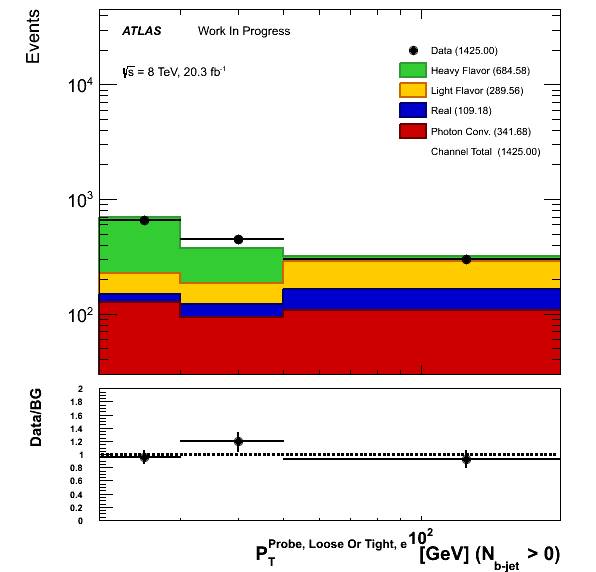
\includegraphics[width=0.45\columnwidth]{figures/fakes_bkg/CRs/SameSignElectronMuon/Scaled/coarse/ProbeLooseORTightElectronPtBJetGt0FakeRate_histratio.png}
%}
%\vspace{-10mm}\caption{Scaled...Transverse momentum distributions \pt\ of tight probe electron (top) and loose or tight probe electrons (bottom) passing signal selection criteria in the Same-Sign $e-\mu$ control region without any additional requirement on $b$-jets in the event (left) and at least one $b$-jet (right).
%The amount observed in data (black points) corresponds to $n$ (bottom) and $n_{\textrm{Tight}}$ (top) in Eq.~\ref{eq:fakerate}. 
%Meanwhile, the contribution determined in MC to come from real leptons (blue), photon conversion (red), heavy flavor (green) and light
%flavor (orange) are shown stacked on top of each other.
%The difference between the data and MC does not effect the data-driven
%fake estimate but may have an impact on the composition estiamte.
%}
%\label{fig:fakeEff_CRs_electron_stacked_scaled}
%\end{figure}


\begin{table}[ht!]
\centering
\begin{tabular}{|lc|ccc|}
    \hline
    \multicolumn{5}{|c|}{\bf{Control regions}}   \\ \hline \hline
    PC subtracted &$N_{b-jet}$  &{HF} &{PC} &{LF} \\ \hline
    yes &--- &$57\pm 4$\%  &$0$\% &$43\pm 6$\% \\
    yes &$N_{b-jet}>0$  &$75\pm 5$\% &$0$\% &$25\pm 3$\% \\ \hline
    no &--- &$22\pm 3$\% &$61\pm 13$\% &$17\pm 3$\% \\
    no &$N_{b-jet}>0$  &$43\pm 3$\% &$42\pm 6$\% &$15\pm 2$\% \\ 
    \hline
	
\end{tabular}




\caption{
Composition of fake electrons taken from  MC events in the same-sign electron-muon dilepton control regions
used to extract electron fake rates. The composition is split as either Heavy Flavor (HF), Photon
Conversion (PC), and Light Flavor (LF) are shown. In the ``PC subtracted'' case, the PC component
has been explicitly removed.  This corresponds to the scenario ultimately used in the
fake rate estimation.
}
\label{table:CompositionElectronCR}
\end{table}

\begin{table}[ht!]
\centering
    \begin{tabular}{|l||cc|}
    \hline 
    \multicolumn{3}{|c|}{\bf{Pre-selection and signal regions}}   \\ 
    & Heavy Flavor & Light Flavor \\
    \hline \hline
    \hline

    Pre-selection &$53.7 \pm 9.4$\% & $46.3\pm 10.0$\% \\
    0 SFOS &$80.2 \pm 19.9$\% & $19.8\pm 11.8$\% \\
    1 SFOS &$52.4 \pm 12.5$\% & $47.6\pm 11.9$\% \\
    2 SFOS &$47.7 \pm 16.1$\% & $52.3\pm 23.3$\% \\
    \hline


  \end{tabular}
  








\caption{
Composition of fake electrons taken from  MC events in the event pre-selection and regions close to the signal regions used in the analysis. 
The composition is split as either Heavy Flavor (HF) or Light Flavor (LF). 
}
\label{table:CompositionElectronSR}
\end{table}


\begin{table}[ht!]
\centering
    \begin{tabular}{|lc|ccc|}
    \hline
    \multicolumn{5}{|c|}{\bf{Control regions}}   \\ \hline \hline
    PC subtracted &$N_{b-jet}$  &{HF} &{PC} &{LF} \\ \hline
    yes &--- &$89\pm 4$\% &$0$\% &$11\pm 1$\% \\
    yes &$N_{b-jet}>0$  &$95\pm 3$\% &$0$\% &$4\pm 1$\%\\ \hline
    no &--- &$89\pm 4$\% &$0$\% &$11\pm 1$\% \\
    no &$N_{b-jet}>0$  &$95\pm 3$\% &$0$\% &$4\pm 1$\%\\ 
    %\color{yellow!70!black}\met\ $>10$GeV &\color{yellow!70!black}$N_{b-jet}>1$  &\color{yellow!70!black}91\% &\color{yellow!70!black}0\% &\color{yellow!70!black}9\% \\ 
    \hline
  \end{tabular}
  

\caption{
Composition of fake muons taken from  MC events in the event pre-selection and regions close to the signal regions used in the analysis. 
The composition is split as either Heavy Flavor (HF), Photon
Conversion (PC), and Light Flavor (LF) are shown. The photon conversion component
is measured to be negligible. No PC subtraction is performed.
}
\label{table:CompositionMuonCR}
\end{table}

\begin{table}[ht!]
\centering
    \begin{tabular}{|l||cc|}
    \hline 
    \multicolumn{3}{|c|}{\bf{Pre-selection and signal regions}}   \\ 
    & Heavy Flavor & Light Flavor \\
    \hline \hline
    \hline

    Pre-selection &$78.9 \pm 10.0$\% & $21.1\pm 4.6$\% \\
    0 SFOS &$96.7 \pm 21.0$\% & $3.3\pm 3.7$\% \\
    1 SFOS &$77.4 \pm 14.1$\% & $22.6\pm 7.2$\% \\
    2 SFOS &$77.3 \pm 15.9$\% & $22.8\pm 7.1$\% \\
    \hline


  \end{tabular}
  








\caption{
Composition of fake muons taken from  MC events in the same-sign muon-muon dilepton control regions
used to extract the muon fake rates. The composition is split into either Heavy Flavor (HF) or Light Flavor (LF). 
}
\label{table:CompositionMuonSR}
\end{table}

\clearpage
\subsubsection{Fake lepton background validation}

A Monte Carlo closure test of the generalized matrix method is performed. The fake rates are computed from MC samples in the dilepton control regions defined in section~\ref{sec:fakecomposition}, and the method is then applied on the most important MC samples contributing to the event pre-selection: $Z$+jets and $t\bar{t}$. The event pre-selection is used for this test, because the statistics available for the MC samples containing fake leptons in the signal region is too small to be able to draw any conclusion. Figure~\ref{fig:MCFakeRatesClosure}, show the MC fake rates obtained from the CR, while figure~\ref{fig:MCClosureCheckMatrixMethod} show the MC agreement with the MC events reweighted using the generalized matrix method in the event pre-selection region, for the third-leading lepton $\pt$ and the $\met$ distribution. As it can be seen the shape agreement and the overall normalization are pretty good, showing that the matrix method is performing well.

\begin{figure}[ht!]
\centering
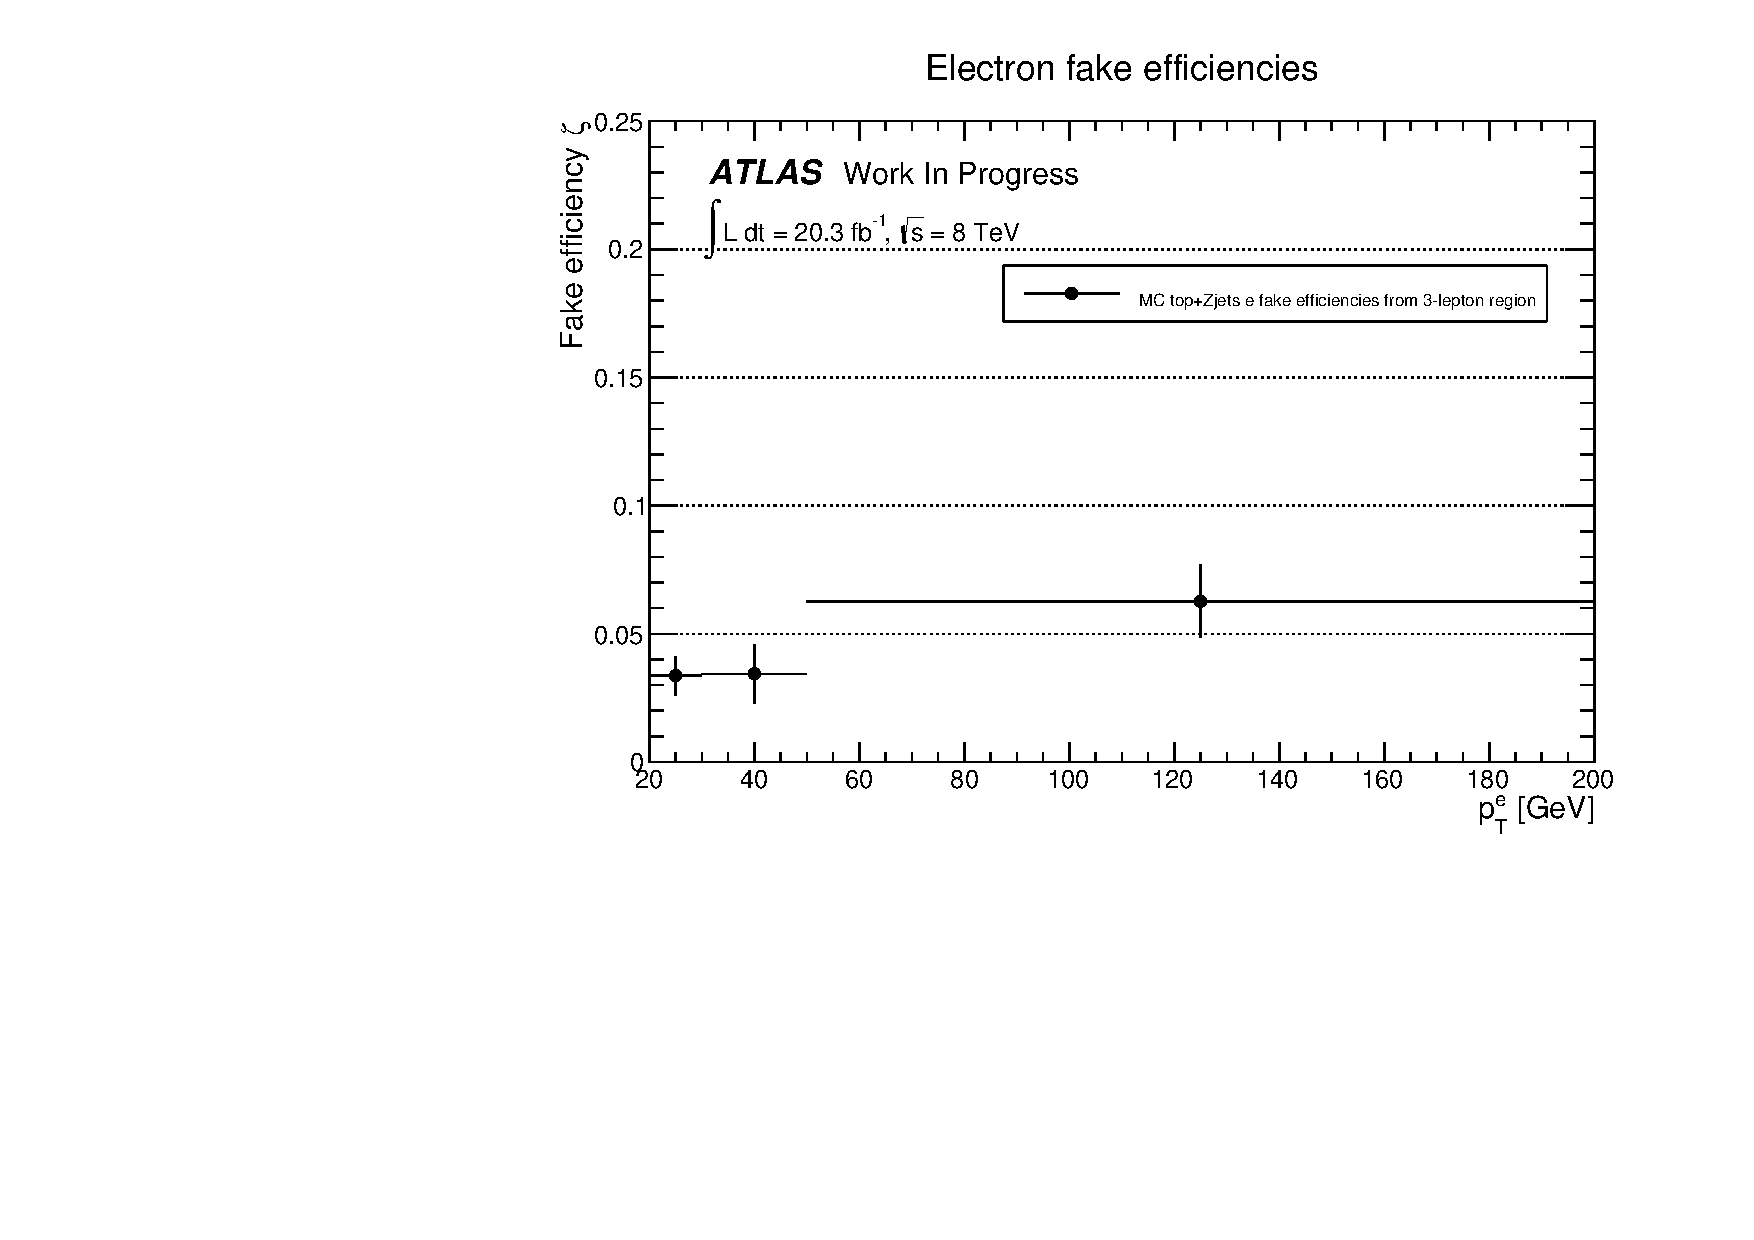
\includegraphics[width=0.42\columnwidth]{figures/ClosureCheck_MatrixMethod/ElFakeRates_MC_topZjets_new.pdf}
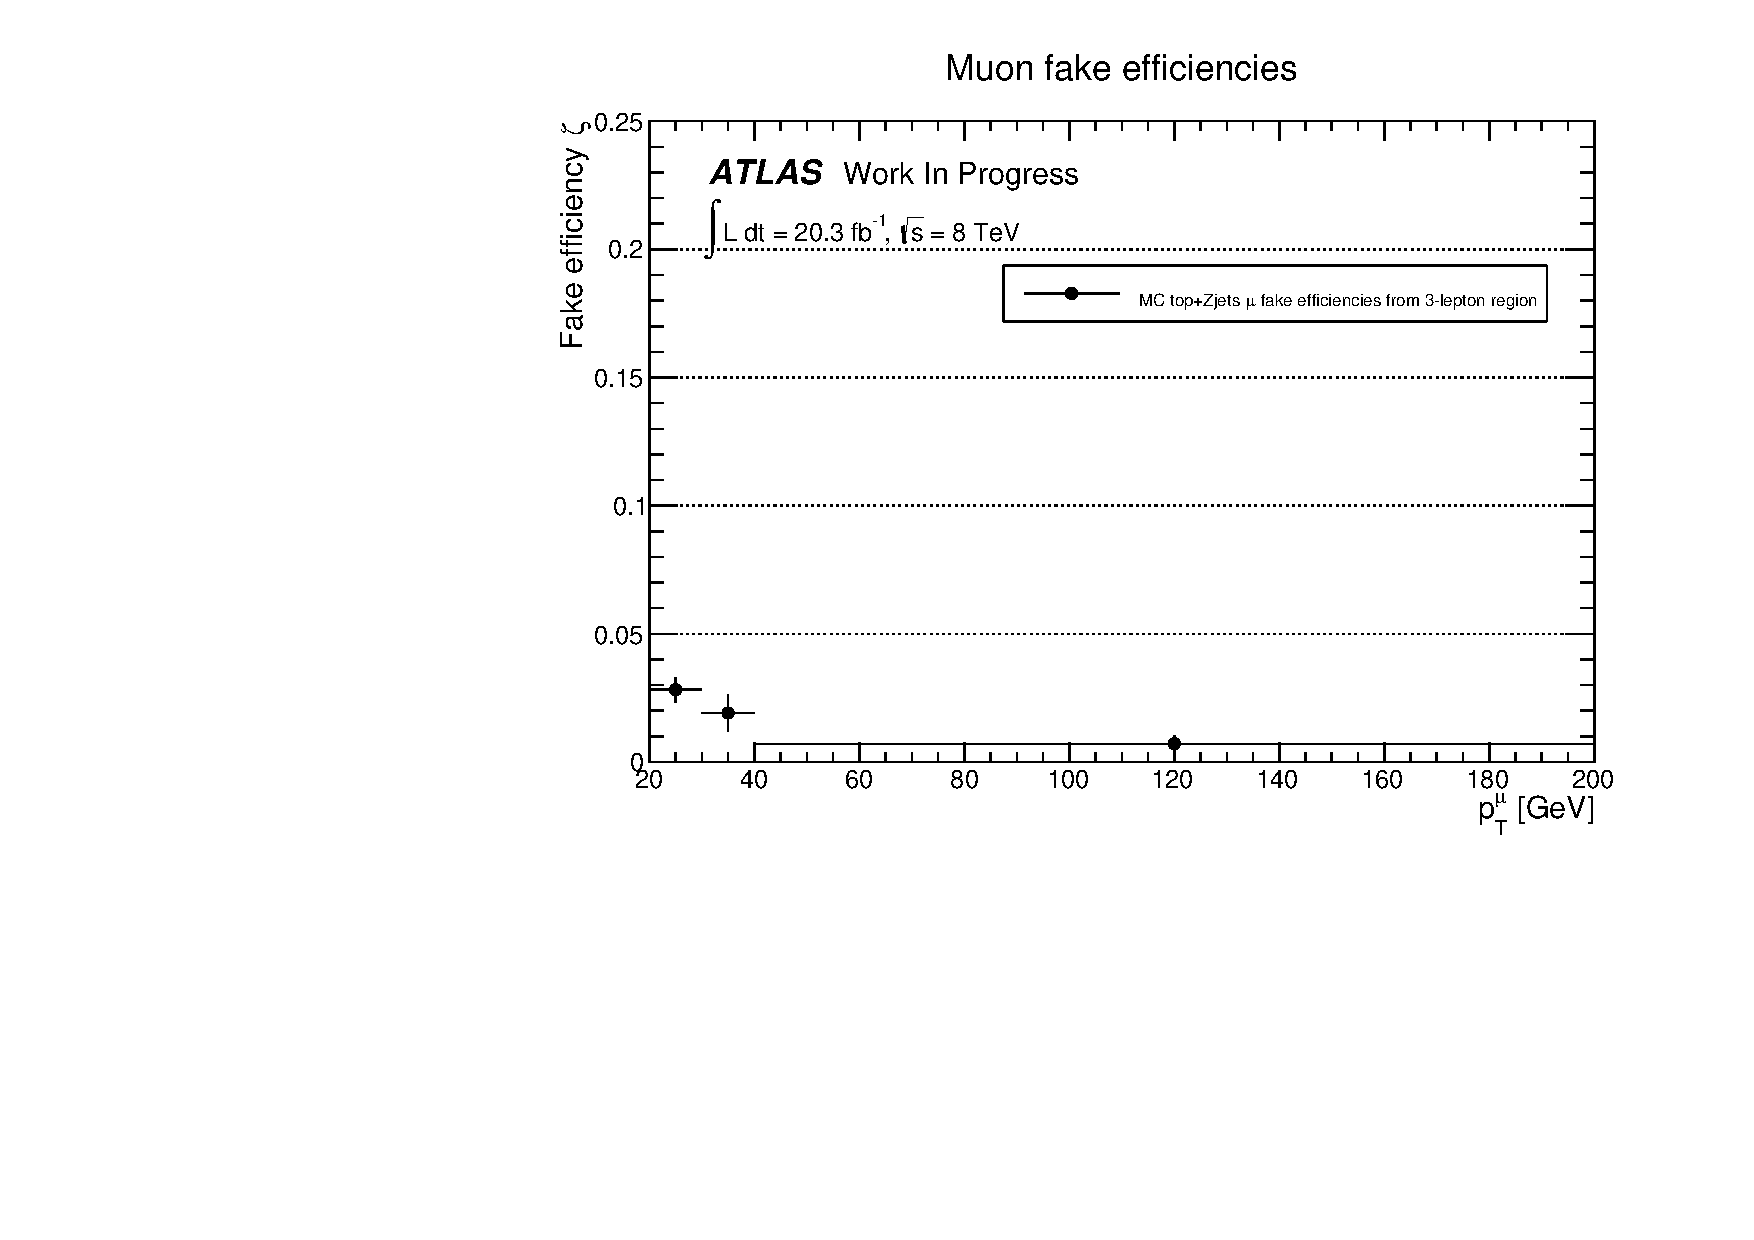
\includegraphics[width=0.42\columnwidth]{figures/ClosureCheck_MatrixMethod/MuFakeRates_MC_topZjets_new.pdf}
\caption{Distribution of the fake rates obtained from MC samples in the dilepton control regions. The errors shown here are statistical only. These rates are used to performed a MC closure check of the global matrix method.}
\label{fig:MCFakeRatesClosure}
\end{figure}

\begin{figure}[ht!]
\centering
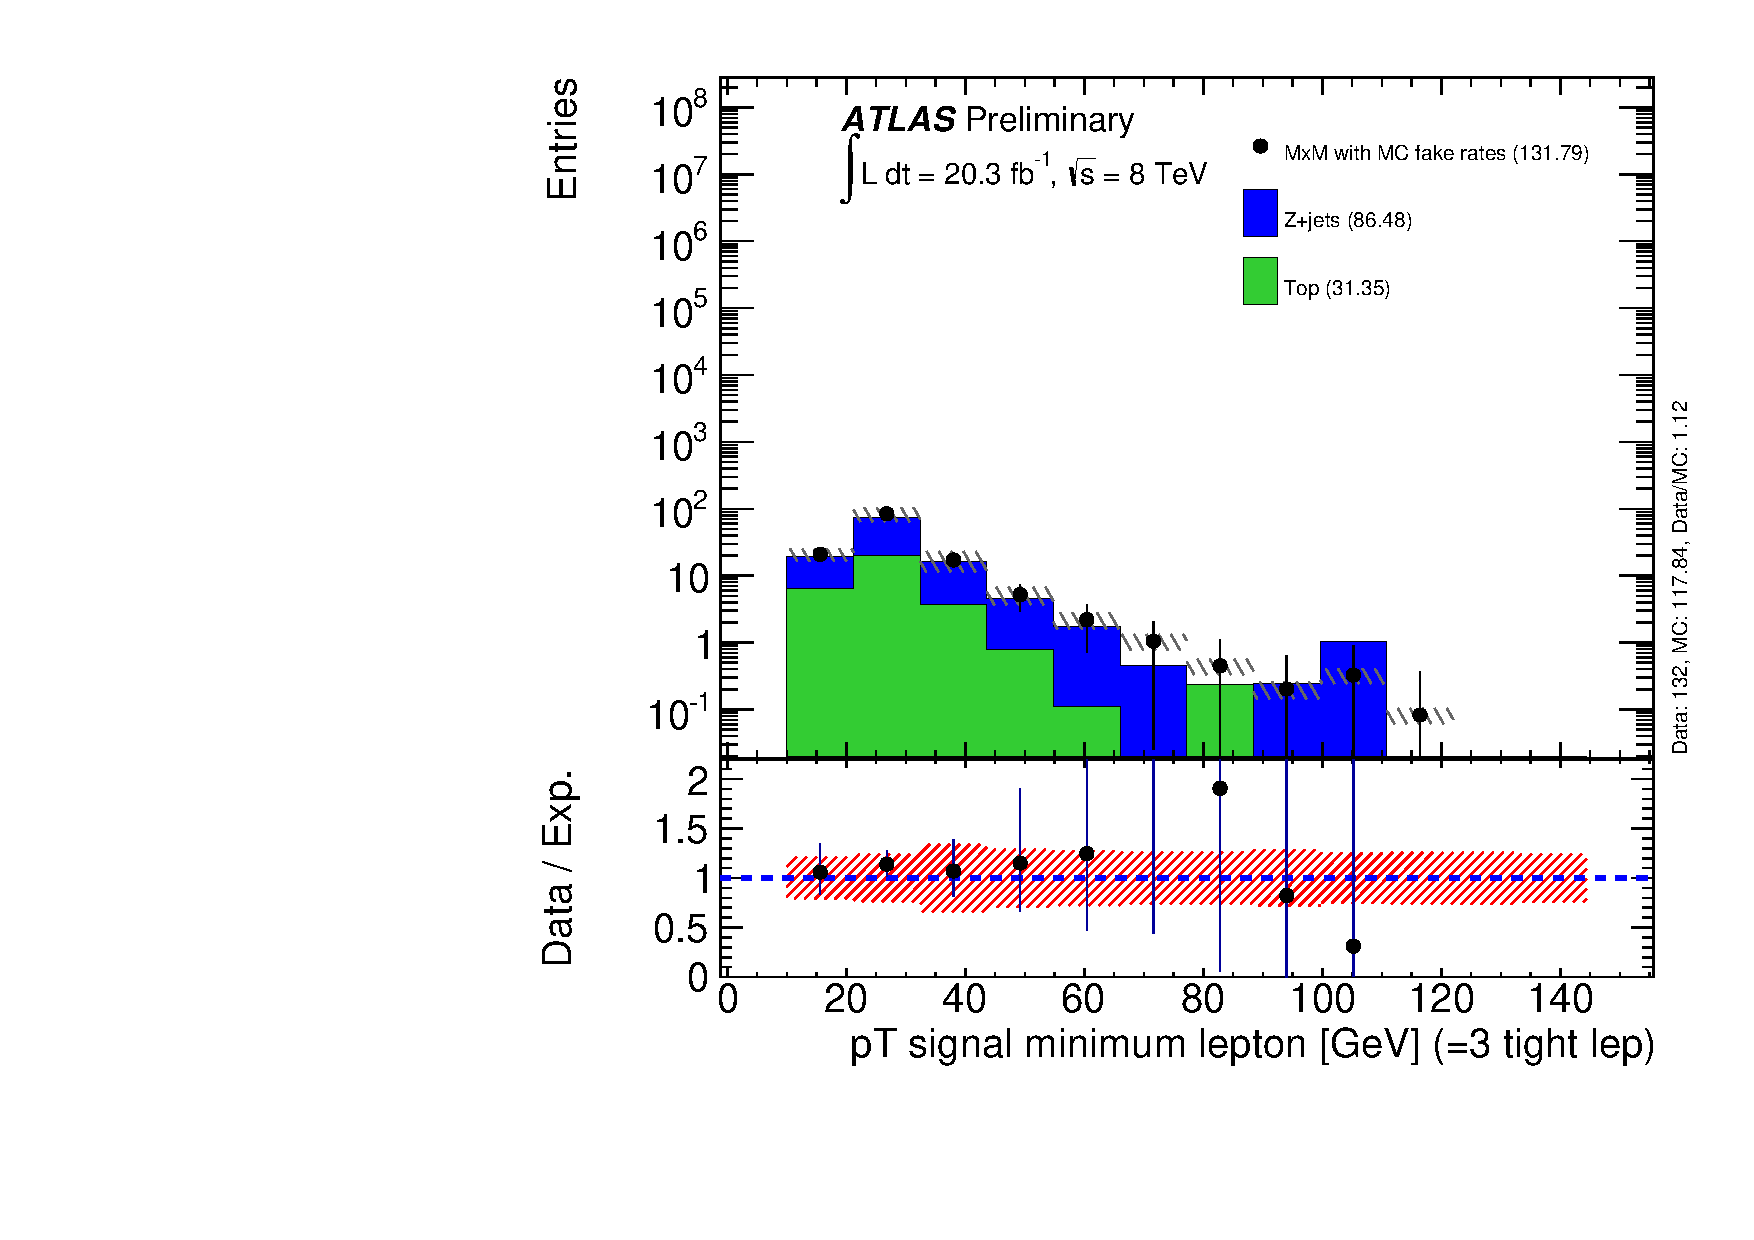
\includegraphics[width=0.42\columnwidth]{figures/ClosureCheck_MatrixMethod/PtThirdLepSignal_TTT_total_new.pdf}
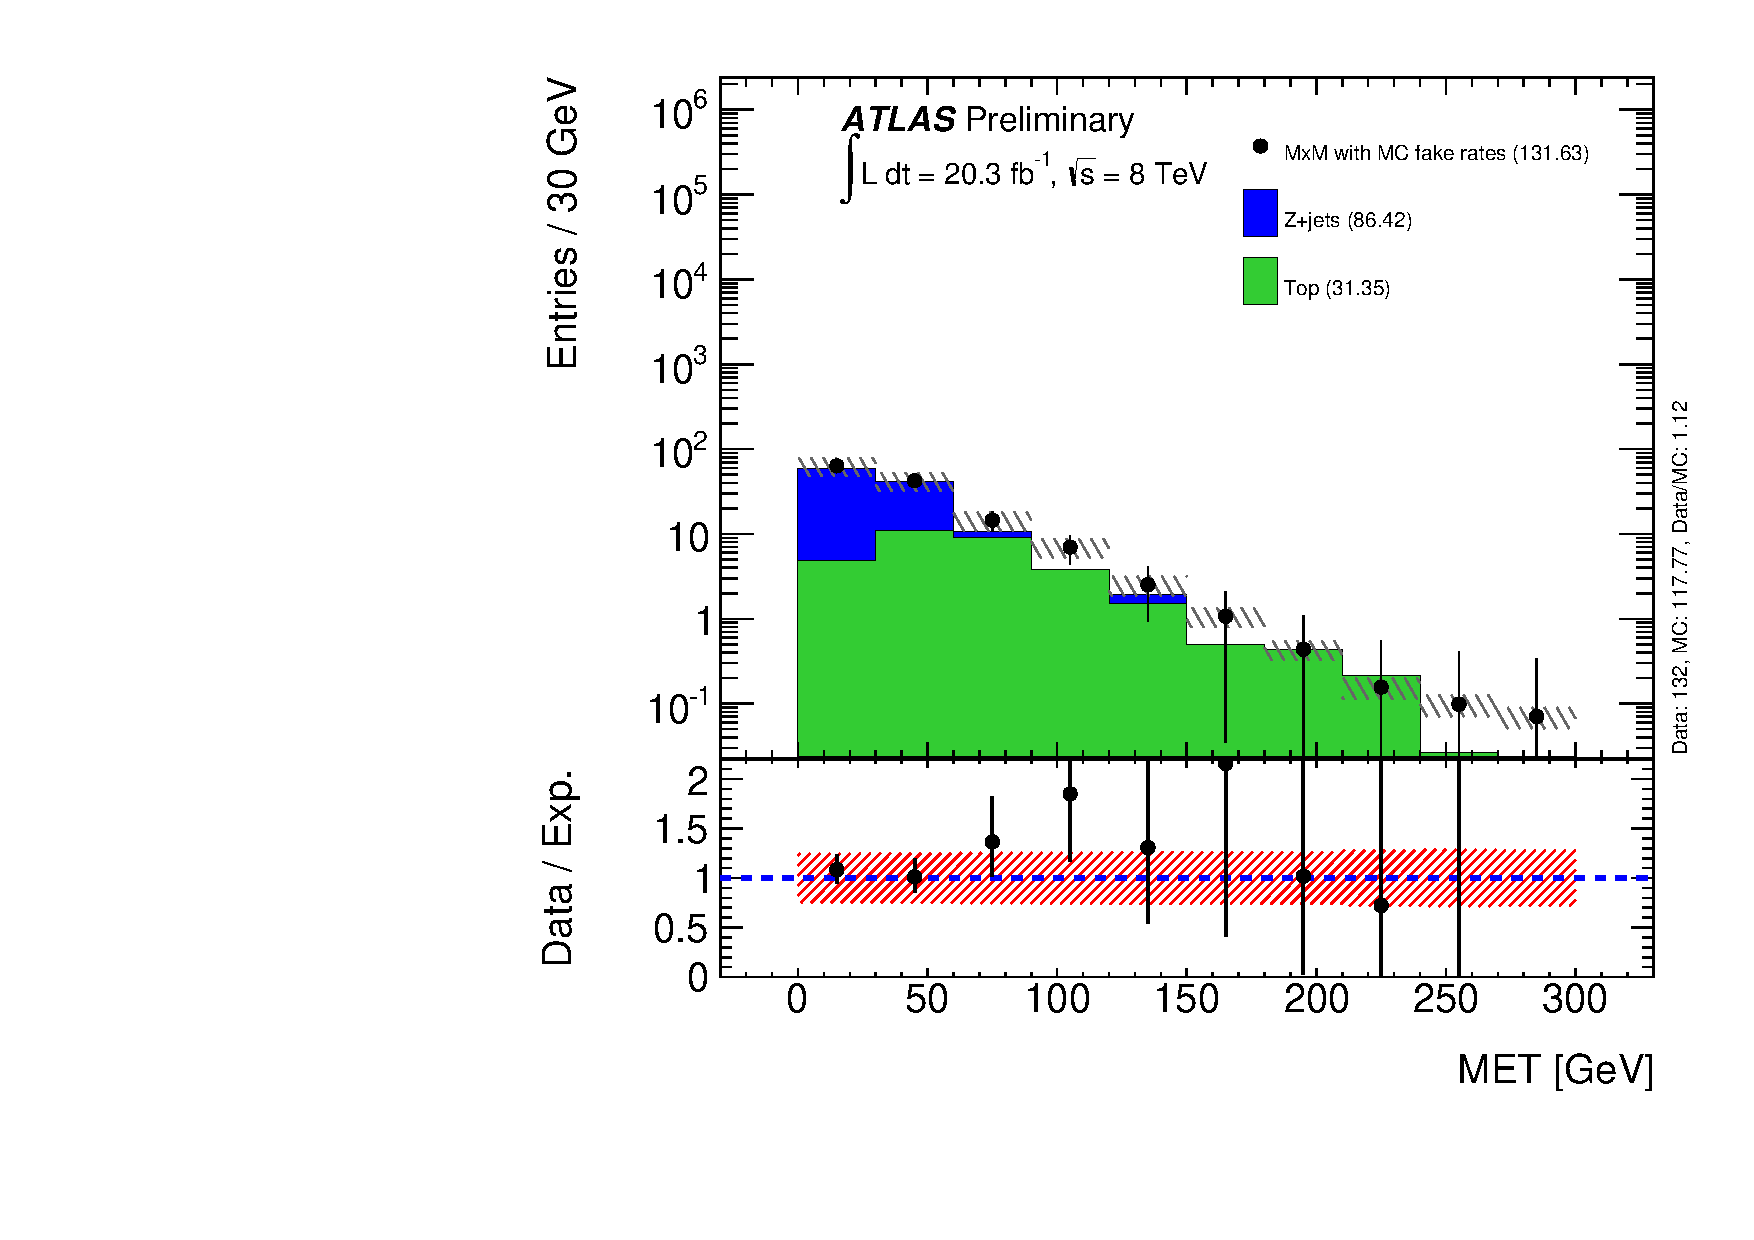
\includegraphics[width=0.42\columnwidth]{figures/ClosureCheck_MatrixMethod/VR_PMET_lepTTT_total_new.pdf}
\caption{Distributions of the third leading lepton $\pt$ and $\met$ in the event pre-selection region, for $Z$+jets and $t\bar{t}$, compared to events from these samples reweigthed using the global matrix method and the rates shown in Figure~\ref{fig:MCFakeRatesClosure}. Good agreement is observed}
\label{fig:MCClosureCheckMatrixMethod}
\end{figure}




The ability of the generalized matrix method just described to model accurately
the fake lepton background is tested in a control region designed to be enhanced
in the fake lepton background while mainitaining orthogonality with the signal
regions described in Section~\ref{sec:signal_regions}. The control region 
starts by using the event pre-selection region described in Section~\ref{sec:preselection}. To reduce contamination in the 
control region from the $WZ$ process, it is required that none
of the three leptons selected form a Same-Flavor Opposite-Sign lepton pair.
Finally, to ensure orthogonality with the signal regions which require that no
$b$-tagged jets are present in the event, this control region requires
the presence of at least one $b$-tagged jet in the event. 

This control region
is clearly dominated by the data-driven fake lepton background as can
be seen in Fig.~\ref{fig:FakeCR} and in Table~\ref{tab:FakeCR}. 
Furthermore, Table~\ref{tab:FakeCR} shows good agreement between data
and the fake background modeling on the total event yield, which is within 
the statistical uncertainties.  One can even see from
Fig.~\ref{fig:FakeCR} that the shape description does a reasonable job,
although the statistical uncertainty is a bit too large to draw strong conclusions.
One can also see that the systematic uncertainty easily covers most
of the differences that are observed. Thus, we conclude that the fake background
description is working and may be used in our signal regions.  Especially since
the fake background is most important in the 0 SFOS region (described in more
detail in Section~\ref{sec:signal_regions}) which differs primarily from this
control region only by the $b$-veto requirement.




\begin{figure}[ht!]
\centering
\includegraphics[width=0.3\columnwidth]{figures/Fake_CR/LeadingLeptonPt_histratio.eps}
\includegraphics[width=0.3\columnwidth]{figures/Fake_CR/SubleadingLeptonPt_histratio.eps}
\includegraphics[width=0.3\columnwidth]{figures/Fake_CR/MinimumLeptonPt_histratio.eps}
\includegraphics[width=0.3\columnwidth]{figures/Fake_CR/MET_Et_histratio.eps}
\includegraphics[width=0.3\columnwidth]{figures/Fake_CR/NBTaggedJets_histratio.eps}
\includegraphics[width=0.3\columnwidth]{figures/Fake_CR/NJets_histratio.eps}
\includegraphics[width=0.3\columnwidth]{figures/Fake_CR/NMuons_histratio.eps}
\caption{Distributions in a control region designed to study the data-driven fake lepton background estimate.  The selection used is as follows: Event pre-selection + 0 SFOS + at least 1 $b$-jet.  Good agreement is observed}
\label{fig:FakeCR}
\end{figure}

\begin{table}[ht!]
\centering
\begin{tabular}{|c||c|c|c|c|}
\hline
 & Event Yield\\ 
\hline\hline
$WZ$ &  $0.338 \pm 0.021$\\ 
$ZZ$ &  $0.0747 \pm 0.0064$\\ 
$Z\gamma$ &  $0.0058 \pm 0.0058$\\ 
$ZWW+ZZZ$ &  $0.026 \pm 0.005$\\ 
$t\bar{t}+V$ &  $3.228 \pm 0.039$\\ 
Fake (data-driven) &  $10.91 \pm 0.73$\\ 
$WWW$ &  $0.1431 \pm 0.0052$\\ 
\hline
Expected Background &  $14.58 \pm 0.73$\\ 
Expected Signal + Background &  $14.72 \pm 0.73$\\ 
\hline
Observed Data &  $18.0 \pm 4.2$\\ 
\hline
\end{tabular}

\caption{Expected and observed yields for the fake lepton control region.}
\label{tab:FakeCR}
\end{table}


